\input{./preamble.tex}
\input{./code_listings.tex}

\newcommand{\bolditalic}[1]{\textbf{\textit{#1}}}

\title{ML Course HSE}


\begin{document}
\author{
\href{https://github.com/danilpavlov/latex_lib/tree/main/univer/4sem/PIAA}{Ссылка} на .tex файлы и все-такое}
\maketitle
\tableofcontents
\newpage

\section{Основные определения. Типы задач.}
    \href{https://www.youtube.com/watch?v=QVs8QjuAN74&list=PLEqoHzpnmTfChItexxg2ZfxCsm-8QPsdS}{Курс «Машинное обучение 1». Лекция 1 (Евгений Соколов)}\\

    \begin{definition}
        \textbf{Объект} (обозначается как $x$) $-$ то для чего мы делаем прогнозы / анализ \\
        В случае с рекомендацией музыки, объект $-$ пара пользователь-трек.\\
        $\mathbb{X}$ $-$ множество объектов.
    \end{definition}

    \begin{definition}
        \textbf{Ответ (целевая переменная, target)} (обозначается как $y$) $-$ что мы предугадываем.\\
        В примере: какую долю трека пользователь послушает. $y \in [0, 1]$\\
        $\mathbb{Y}$ $-$ множетсво ответов.\footnote{
    Будем писать: $\mathbf{X} = \{(x_i, y_i) \}_{i=1}^\ell$, где $\ell$ $-$ размер обучающей выборки (сама обучающая выборка (train set), очевидно, $-$ $\mathbf{X}$). }\\
    \end{definition}

    \\


    \textbf{Признаки (факторы, features)} $-$ характеристики объекта.\footnote{Будем писать: $x$ $=$ $(x_1 ... x_d)$
        где $x$ - объект, а $(x_1 ... x_d)$ - его признаки (размера $d$).}\\

    \underline{Типы признаков:}
    \begin{enumerate}
        \item \textbf{Бинарные} (т.е. $\in \{0, 1\}$)
        \item \textbf{Числовые} (т.e. $\in \mathbb{R}$)
        \item \textbf{Категориальные} (по-статистически \textit{номинальные}) (т.е. $\in \{C_1 ... C_n \}$ $-$ неупорядоченные и без метрики) \\Например: жанр песни
        \item \textbf{Порядковые} (т.е. $\in \{C_1 ... C_n \}$ - с частичным порядком) \\Например, тип альбома: сингл, полный альбом...
        \item \textbf{Set-valued} (т.е. $\subset C$, где $C = \{c_1 ... c_n  \}$) * его можно закодировать через one-hot кодирование
        \item \textbf{Со сложной структурой} \\Например: картинка, текст, звук...\\\\
    \end{enumerate}

    \underline{$\mathbb{Y}$ определяет тип задачи}
    \begin{enumerate}
        \item \textbf{Регрессия}: $\mathbb{Y} = \mathbb{R}$ (ответ - число)
        \item \textbf{Классификация}: $\mathbb{Y} = \{1 ... k \}$, причем $\{1 ... k \}$ без порядка [элементы множества - классы] (множество ответов конечное) \\Например: по треку определить его жанр (множество жанров конечно)\\
        \begin{itemize}
            \item \textbf{Бинарная классификация}: $\mathbb{Y} = \{-1, +1\}$
            \item \textbf{Multi-label классификация}: $\mathbb{Y} = \{-1, +1 \}^k$
        \end{itemize}
    
        \todo[inline]{Задачи \bolditalic{Регрессии} и \bolditalic{Классификации} являются основными типами задач \bolditalic{обучения с учителем (supervised learning)} (т.е. в $\mathbb{X}$ правильные ответы)}
        
        \item \textbf{Кластеризация}: $\mathbb{X}$ $=$ $\{(x_i) \}_{i=1}^\ell$. Задача разбить объекты на кластеры.
        \item \textbf{Понижение размерности}: Задача найти меньшое число признаков, которое по своей характеристике будет похоже на изначальный набор признаков.

        \todo[inline]{Задачи \bolditalic{Кластеризации} и \bolditalic{Понижения размерности} являются основными типами задач \bolditalic{обучения без учителя} (т.е. есть какая-то выборка \underline{без} правильных ответов)}
    \end{enumerate}
    

    \begin{definition}
        $\alpha \in \mathcal{A}$ $-$ \textbf{семейство моделей}\\
    $\alpha: \mathbb{X} \rightarrow \mathbb{Y}$ $-$ \textbf{модель}\\

    Пример моделей: $\mathcal{A} = \{\alpa(x) = \omega_0 + \omega_1x_1 + ... + \omega_dx_d \quad | \quad \omega_0 ... \omega_d \in \mathbb{R} \}$ $-$ \textit{семейство линейных моделей}\\
    \end{definition}
    

    \begin{definition}
        \textbf{Функция потерь}: $L : \mathbb{X} \times \mathbb{Y} \rightarrow \mathbb{R}_+$ $-$ функция, которая оценивает ошибку модели (Чем больше функция потерь неправа, тем больше число оно вернет).\\

        Примеры функций потерь:
        ($\ast$ $z$ $-$ выход модели)
        \begin{itemize}
            \item $L(y, z) = (y - z)^2$ $-$ \textit{для регрессии (\textbf{квадратичная функция потерь})}
    
            \item $L(y, z) = [y \neq z]$ $-$ \textit{для классификации} (\textbf{бинарная функция потерь})\\
            $\ast$ в квардатных скобках - логическое высказывание\\
    \end{itemize}
    \end{definition}
    

    \begin{definition}
        \textbf{Функционал\footnote{Функционал $-$ функция которая принимает функцию (в данном примере она принимает модель)} ошибки}: $Q(\alpha, \mathbf{X}) = \frac{1}{\ell} \sum\limits_{i=1}^\ell L(y_i, \alpha(x_i))$\\
        $\ast$ $y_i$ $-$ правильный ответ для $x_i$
    \end{definition}


    \begin{definition}
        \textbf{Задача обучения}:\\

        \begin{center}
            $Q(\alpha, \mathbf{X}) \longrightarrow \min\limits_{\alpha \in \mathcal{A}}$
        \end{center}
        
        
    \end{definition}

\newpage
\section{Линейная регрессия.}    
    \href{https://www.youtube.com/watch?v=MA66hFXaq7o&list=PLEqoHzpnmTfChItexxg2ZfxCsm-8QPsdS&index=2}{Курс «Машинное обучение 1». Лекция 2 (Евгений Соколов)}\\

    \begin{center}
        \textbf{Задача регрессии}\\
        
        $\mathbb{Y} = \mathbb{R}$
    \end{center}

    \subsection{Модель линейной регрессии}
        \begin{center}
            $\alpha(x) = \omega_0 + \omega_1x_1 + ... + \omega_dx_d$ \quad $=$ $\omega_0 + \sum\limits_{j=1}^d \omega_jx_j$ \quad $= \omega_0 + <\omega, x>$ \quad $= <\omega, x>$  \footnote{$\omega_j$ называют \textit{весами (или коэффициентами, параметрами)}. $\omega_0$ называют \textit{свободным коэффициентом (bios)}}

            $\ast$ Данная модель имеет $(d+1)$ число параметров.
        \end{center}
        
    \subsection{Области применимости модели}
        $x$ $-$ квартира в Москве; $y$ $-$ ее рыночная стоимость.

        $\alpha(x) = \omega_0 + \omega_1 \cdot (площадь) + \omega_2 \cdot $(кол-во комнат)$  + \omega_3 \cdot$ (расстояние до метро)\\
        
        \todo[inline]{Заметим, что при увеличении площади, цена (модель) будет расти только засчет $\omega_1$. Это странно, поскольку признаки должны влиять в совокупности на стоимость квартиры (например, если квартира находиться близ метро, при росте площади цена должна расти быстрее, нежели в случае, когда квартира находится далеко от метро). \bolditalic{Поэтому, если мы хотим учитывать сложные взаимодействия признаков, лучше использовать другие модели.} }\\

        Тем не менее, линейный модели в некоторых случаях могут быть очень адекватными:
        \begin{enumerate}
            \item \textbf{Категориальные признаки}.\\
                \textbf{Пример}:\\

                $x_i$ $-$ район.\\
                $C = \{c_1 ... c_n \}$ $-$ мн-во значений признака.\\

                
                $b_1(x), ... b_n(x) $ $-$ новые признаки, где $b_j(x) = [x_i = c_j]$\\
                Очевидно\footnote{Такое кодирование называется one-hot}, что $b_1(x), ... b_n(x) $ $= 1$\\

                $\alpha(x) = \omega_0 + \omega_1 \cdot [x_1 = c_1] + \omega_2 \cdot [x_1 = c_2] + ... \omega_n \cdot [x_1 = c_n] + .....$
                
            \newpage
            \item \textbf{Бинаризация числовых признаков}.\\
                \textbf{Пример}:
                
                \begin{tikzpicture}
                \begin{axis}[
                  xlabel={Расстояние до метро},
                  ylabel={Цена квартиры},
                  axis lines=left,
                  enlargelimits=upper,
                  tick align=inside,
                  domain=0:10,
                  samples=100,
                  no markers,
                  smooth
                  ]
                  \addplot[blue] {5*exp(-(x-4)^2/10)}; % Формула нормального распределения
                \end{axis}
                \end{tikzpicture}

                \begin{center}
                    $\omega_j \cdot$ (расстояние до метро)
                \end{center}
    
                \begin{tikzpicture}
                \draw[->] (0,0) -- (10,0) node[right] {Расстояние до метро}; % Рисуем ось Х
                \foreach \x in {1,2,...,9} % Добавляем точки на прямую
                    \filldraw (\x,0) circle (2pt);
                \draw (5.2,0) -- (5.2,0.5) node[above] {t1}; % Разбиваем прямую на секторы с помощью вертикальных черт
                \draw (8.3,0) -- (8.3,0.5) node[above] {t2};
                \draw (9.5,0) -- (9.5,0.5) node[above] {t3};
                \end{tikzpicture}

                \begin{center}
                    $t_0 = - \infty$\\
                    $t_{n+1} = + \infty$\\

                    $b_i(x) = [t_{i-1} \leq x_1 < t_{i}]$\\

                \end{center}
                
                \begin{center}
                    \large{$\alpha(x) = \omega_1 [t_0 \leq x_1 < t_1] + ... \quad \omega_{n+1}[t_n \leq x_1 < t_{n+1}] + ....$}

                \end{center}

                \todo[inline]{Для линейных моделей признаки нужно готовить так, чтобы модель была \bolditalic{осмысленной} }
        \end{enumerate}

        \subsection{Измерение ошибки в задачах регрессии}

            \begin{enumerate}
            \item \bolditalic{$L(y, z) = (y - z)^2$ $-$ квадратичная функция потерь.}\\
                MSE ($\alpha, \mathbf{X}$)\footnote{MSE $-$ mean squared error}$=$ $\frac{1}{\ell} \sum\limits_{i=1}^\ell (\alpha(x_i) - y_i)^2$\\

                У данного функционала есть проблемы:
                \begin{itemize}
                    \item Допустим, мы предсказываем стоимость квартиры. Тогда прогнозы в рублях ($\alpha$), целевая переменная тоже в рублях ($y$), тогда при возведении в квадрат их разности мы получим рубли в квадрате. \textit{Не совсем понятно, что такое рубли в квадрате...}\\

                    Тогда люди придумали модификацию данного метода: RMSE (root mean squared error).

                    \begin{center}
                        $RMSE$($\alpha, \mathbf{X}$)$=$ $\sqrt{MSE(\alpha, \mathbf{X})}$
                    \end{center}
                    \end{itemize}
    
                
                    \textbf{Коэффициент детерминации}:\\
                        \begin{center}
                            \large{$R^2(\alpha, \mathbf{X})$ $=$ $1 - \frac{MSE(\alpha, \mathbf{X})}{\sum\limits_{i=1}^\ell (y_i - \bar{y})^2}$}
                            
                        \end{center}
                        \begin{center}
                             $\ast$ В знаменателе дисперсия
                        \end{center}
                    Коэффициент детерминации нормирован, то есть:
                    \begin{itemize}
                        \item Если $\alpha(x)$ идеальна $\longrightarrow$ $R^2 = 1$
                        \item Если $\alpha(x)$ константа $\longrightarrow$ $R^2 = 0$\\
                    \end{itemize}

            \item \bolditalic{$L(y, z) = |y - z|$}\\
                \begin{center}
                    \large{MAE$(\alpha, \mathbf{X})$\footnote{mean absolute error} $= \frac{1}{\ell}\sum\limits_{i=1}^\ell |\alpha(x_i) - y_i|$}
                \end{center}

                \begin{table}[ht]
                \centering
                \begin{tabular}{|c|c|c|c|}
                \hline
                $y$ & $\alpha(x)$ & $(y - \alpha(x))^2$ & $|y - \alpha(x)|$ \\
                \hline
                $1$ & $2$ & $1$ & $1$\\
        
                (выброс)$1000$ & $2$ & $996004$ & $998$\\
                \hline
                $1$ & $1$ & $0$ & $0$\\ 
                
                $1000$ & $3$ & $994009$ & $997$\\
                \hline
                \end{tabular}
                \caption{Сравнение MAE и MSE}
                \end{table}

                \todo[inline]{Таким образом, MAE устойчив к выбросам}

                \begin{center}
                    \bolditalic{Еще пример, почему MAE более устойчив к выбросам} (Из лекции 5)
                    
                \end{center}

                $\alpha_2(x)$ сильнее ошибается на нормальных объектах, но чуть меньше ошибается на выбросе
                \begin{table}[ht]
                    \centering
                    \begin{tabular}{|c|c|c|c|}
                    \hline
                    $y$ & $\alpha_1(x)$ & $\alpha_2(x)$\\
                    \hline
                    $1$ & $2$ & $4$\\
                    \hline
                    $2$ & $1$ & $5$\\
                    \hline
                    $3$ & $2$ & $6$\\ 
                    \hline
                    $4$ & $5$ & $7$\\
                    \hline
                    $5$ & $6$ & $8$\\
                    \hline
                    $\cancel{6}$ $1000$ & $7$ & $10$\\
                    \hline
                    $7$ & $6$ & $10$\\
                    \hline
                    \end{tabular}
                \end{table}

                MSE$({\alpha_1}$) = $1236$ \quad \quad MAE$({\alpha_1}$) = $14.14$\\
                MSE(${\alpha_2}$) = $1164$ \quad \quad MAE$({\alpha_2}$) = $15.43$
                \todo[inline]{Таким образом, если есть вариант похуже предсказания на нормальных объектах, но получше предсказания на одном выбросе, то MSE выбирает его. MAE, в свою очередь, выбриает обратный расклад}
                
                

            \item \textbf{Функция Хубера (Huber loss)}
                \begin{figure}[H]
                    \centering
                    \includegraphics[width=0.5\textwidth]{images/2lecture/HuberLossPlot.png}
                \end{figure}

            \item \textbf{Несимметричные функции потерь}.\\

            Например, квартира стоит 10 миллионов, а модель предсказала, что 5. По итогу, мы потеряем много денег. Идея в том, чтобы давать бôльшие штрафы за недопрогноз, чем перепрогноз

            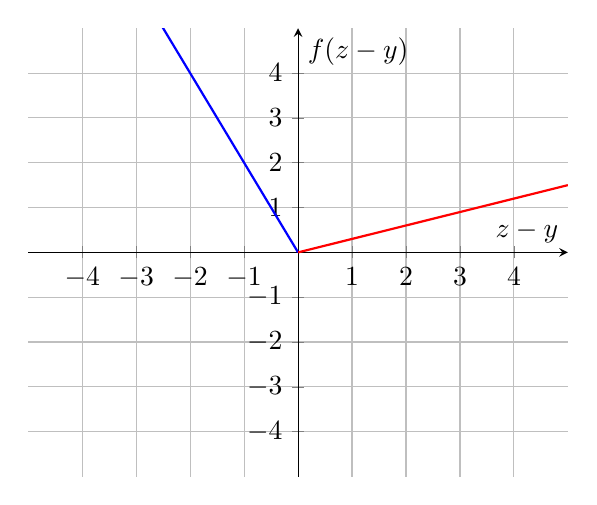
\begin{tikzpicture}
            \begin{axis}[
                xlabel={$z - y$},
                ylabel={$f(z - y)$},
                axis lines=middle,
                xmin=-5,
                xmax=5,
                ymin=-5,
                ymax=5,
                xtick={-4,-3,-2,-1,1,2,3,4},
                ytick={-4,-3,-2,-1,1,2,3,4},
                grid=both,
                legend pos=outer north east,
            ]
            \addplot[domain=-5:0, samples=100, blue, thick] {-2*x};
            \addplot[domain=0:5, samples=100, red, thick] {0.3*x};
            \end{axis}
            \end{tikzpicture}

                
            \item \textbf{MSLE (mean squared logarithm error)}: $L(y, z) = $ $(\log(z+1) - \log(y+1))^2$

            \item $L(y, z) = |\frac{y - z}{y}|$\\

                \begin{center}
                    \large{MAPE($\alpha, \mathbf{X}$)\footnote{mean absolute percentage error} $= \frac{1}{\ell}\sum\limits_{i=1}^\ell \frac{|y_i - \alpha(x_i)|}{|y_i|}$}
                \end{center}

            \end{enumerate}



    \subsection{Обучение}
        \begin{center}
            \large{$\frac{1}{\ell}\sum\limits_{i=1}^\ell (<\omega, x_i> - y_i)^2$ $\longrightarrow$ $\min\limits_\omega$}
        \end{center}

        
        \[\mathbf{X} = 
        \begin{bmatrix}
            x_{11} & x_{12} & ... & x_{1d} \\
            ... & ... & ... & ... \\
            x_{\ell1} & x_{\ell2} & ... & x_{\elld} \\
        \end{bmatrix}
        \]

        \[y = 
        \begin{bmatrix}
            y_{1}\\
            ...  \\
            y_{\ell}\\
        \end{bmatrix}
        \]

        \[\omega = 
        \begin{bmatrix}
            \omega_{1}\\
            ...  \\
            \omega_{d}\\
        \end{bmatrix}
        \]

        \begin{center}
            \large{MSE $= \frac{1}{\ell}||\mathbf{X}\omega - y||_2^2$ $\longrightarrow \min\limits_\omega$}
        \end{center}
        
        \[\ast\mathbf{X}\omega  = 
        \begin{bmatrix}
            <\omega, x_1>\\
            ...  \\
            <\omega, x_\ell>\\
        \end{bmatrix}
        \]

        \begin{center}
            \bolditalic{Поиск минимума многомерной функции}\\ 
            $\nabla_\omega$ MSE $= 0$ \\
            $\vdots$\\
            $\omega = (\mathbf{X}^T\mathbf{X})^{-1}\mathbf{X}^Ty$\\
            (формула работает только если $\mathbf{X}$ полного ранга (её ранг равен минимальному из чисел m и n ))
        \end{center}

        \todo[inline]{Заметим, что матрица $\mathbf{X}^T$ имеет размер $d \times \ell$, а матрица $\mathbf{X}$ имеет размер $\ell \times d$. Тогда их произведение будет иметь размер $d \times d$. Сложность его обращения будет $O(d^3)$, т.е. если объект имеет 1000 признаков, для его обращения понадобится $1000^3$ операций...\\
        
        Конечно для MSE этот способ работает, однако для большинства функций потерь в машинном обучение нельзя решить уравнение $\nabla_\omega$ Q $= 0$ в явном виде, поэтому придумали численные решения таких задач (например: градиентный спуск)}

        \subsection{Обобщающая способность модели}\footnote{Обобщающая способность модели $-$ Способность модели работать нормально на новых данных}

            \begin{figure}[H]
                \centering
                
                \caption{Пример переобучения модели}
                \includegraphics[width=1\textwidth]{images/2lecture/OverFitting.png}
                \label{fig:overfitting}

            \end{figure}

            \begin{definition}
                \textbf{Переобучение (overfitting)} $-$ ситуация, когда ошибка на новых данных больше чем на обучающей выборке.\\
            \end{definition}

            \textbf{Способы обнаружения}:
            \begin{enumerate}
                \item \underline{\textbf{Отложенная выборка}}.\\
                    $\mathbf{X} - $ обучающая выборка.\\
                    $\mathbf{X}_{test}$ $-$ тестовая выборка.\\

                    $Q(\alpha, \mathbf{X}) \lessgtr Q(\alpha, \mathbf{X}_{test})$

                \item \underline{\textbf{Кросс-валидация}}.\\
                    \textbf{Идея}:\\
                    Допустим у нас есть обучающая выборка $\mathbf{X}$.\\
                    Делим ее на $K$ число блоков (fold).\\
                    Обозначим k-й блок как $\mathbf{X}^K$, а все блоки кроме k-го как $\mathbf{X}^{\backslash K}$.\\
                    Тогда оценка кросс-валидации считается как:
                    \begin{center}
                        \large{CV $=$ $\frac{1}{K} \sum\limits_{k=1}^KQ(\alpha(x; \mathbf{X}^{\backslash k}), \mathbf{X}^k)$}
                    \end{center}
                    $\ast$ $\alpha(x; \mathbf{X}^{\backslash k})$ означает, что модель обучена на $\mathbf{X}^{\backslash k}$\\

                    \textbf{Замечания:}
                    \begin{enumerate}
                        \item Если размер выборки большой, то CV врятли нужна

                        \item CV требует обучения $K$ моделей
                    \end{enumerate}

                    \textbf{Итоговая модель}:\\
                    \begin{enumerate}
                        \item Обучить на всех данных
                        \item Усреднить $K$ моделей (т.е. $C(x) = \sum\limits_{k=1}^K\alpha(x, \mathbf{X}^{\backslash k})$)
                    \end{enumerate}
                
            \end{enumerate}


\newpage
\section{Продолжение Линейных Моделей. Градиентный спуск.}
    \href{https://www.youtube.com/watch?v=Wwg6dU1pX4A&list=PLEqoHzpnmTfChItexxg2ZfxCsm-8QPsdS&index=3}{Курс «Машинное обучение 1». Лекция 3 (Евгений Соколов)}\\

    \subsection{Борьба с переобучением}
        На рисунке \ref{fig:overfitting} веса $(\omega_j)$ у модели очень большие: $10^6, 10^7, \cdots$\\

        \textbf{Регуляризация} $-$ запрет на большие веса.\\

        Допустим у нас есть функционал $Q(\omega, \mathbf{X})$.\footnote{$Q(\omega, \mathbf{X})$ означает, что модель линейная с набором весов $\omega$}\\
        Добавим к нему слагаемое:  $\lambda||\omega||^2_2$, тогда получим:\\
        \begin{center}
            \large{$Q(\omega, \mathbf{X}) + \lambda||\omega||^2_2 \longrightarrow \min\limits_\omega$},\\
            где $\lambda -$ \textit{коэффициент регуляризации}, а $||\omega||^2_2$ $-$ \textit{регуляризатор}\footnote{$||\omega||_2^2$ = $\sum\limits_{i = 1}^d\omega^2_i$}.\\
        \end{center}
        
        Аналитическое решение будет тогда выглядеть (для случая если Q это MSE):\footnote{$\lambda I$ $-$ единичная матрица с $\lambda$ на диагонали, где $\lambda \geq 0$}\\
        \begin{center}
            $\omega = (\mathbf{X}^T\mathbf{X} + \lambda I)^{-1}\mathbf{X}^Ty$
        \end{center}

        \todo[inline]{При добавлении к $\mathbf{X}^T\mathbf{X}$ матрицы $\lambda I$, итоговая матрица будет \bolditalic{невырожденной}, поскольку $\mathbf{X}^T\mathbf{X}$ точно неотрицательно определенная (т.е. все собственные значение $\geq 0$) и при прибавлении единичной матрицы $\lambda I$ все собственные значения сдвигаются на $\lambda$.\\
        Таким образом, у \bolditalic{этой матрицы гарантированное будет обратная из-за чего можно посчитать аналитическое решение для задачи минимизации} .}

        \todo[color=red!30, inline]{\textbf{\underline{Важное замечание:}}\\
        В $||\omega||^2_2$ не входит $\omega_0$!!!\\
        (Иначе $\alpha(x)$ не сможет быть одного порядка с $y$)}

        \subsubsection{Почему большие веса плохо?}
            \textbf{Пусть есть модель}:\\
            \begin{center}
                $\alpha(x) = 10^6 + 3\cdot10^7\cdot$(площадь) $ - 5\cdot10^6\cdot$ (расстояние до метро) $\cdots$
            \end{center}
            \underline{Чем модель плоха, помимо того, что она переобучена?}\\
            
            Допустим, \textit{площадь} меняется на $0.001$ м$^2$, но прогноз ($\alpha(x)$) меняется на $3 \cdot 10^4$.\\
            
            Значение признака изменилось на совсем немного, однако значение прогноза поменялось значительно. Это означает, что модель неадекватная.\\

        \subsubsection{Как выбирать $\lambda$?}
            \begin{enumerate}
                \item \textbf{По обучающей выборке}: выбираем $\lambda$ при которой ошибка нашей модели на обучающей выборке ($Q(\alpha, \mathbf{X})$) минимальная.\\
                \textbf{Плохо} $-$ оптимально $\lambda = 0$
                    
            \end{enumerate}

            \begin{center}
                \bolditalic{Регуляризатор не обязательно через $L_2$-норму!}\\
                Например, через\footnote{$||\omega||_1$ = $\sum\limits_{j=1}^d|\omega_j |$} $L_1$ норму весов:\\
                $Q(\omega, \mathbf{X}) + \lambda ||\omega||_1 \longrightarrow \min\limits_{\omega}$
            \end{center}
            \todo[inline]{У $L_1$ нормы существует свойство, что при ее использовании на регулялизаторе, некоторые веса будут строго зануляться (на $L_2$ они будут маленькими, но никак не нулевыми), причем чем больше $\lambda$, тем больше будет нулевых весов.}

        \subsubsection{Еще одна проблема линейных моделей}
            Допустим, в $\mathbf{X}$ есть \textit{линейно зависимые признаки}\footnote{Определение линейной зависимости: $\exists \upsilon : \forall x \in \mathbf{X}$ верно, что $<\upsilon, x> = 0$}\\
            $\omega_*$ $-$ лучшие по MSE веса.\\
            \begin{center}
                $<\omega_* + \alpha\upsilon, x>$ = $ <\omega_*, x> + \alpha<\upsilon, x> $ = $<\omega_*, x>$, \\
                т.к. $<\upsilon, x>$ = $0 $
            \end{center}
            Это означает, \bolditalic{решение не единственное}:\\
            \begin{center}
                $\omega_* + \alpha\upsilon$ $\longrightarrow\limits_{\alpha \rightarrow \infty}$ решение, в котором веса все больше и больше.
            \end{center}
            \todo[inline]{\textbf{Мораль}\\
            Если признаки линейно зависимые, это означает, что есть среди всех решений есть те, которые имеют очень большие веса, что означает, что существуют переобученные решения.}

        \subsection{Обучение линейной регрессии. Градиентный спуск.}

            Для MSE (при малом числе признаков ($\leq 100$)): 
            \begin{center}
                $\omega$ = $(\mathbf{X}^T\mathbf{X})^{-1}\mathbf{X}^Ty$
            \end{center}

            \subsubsection{Градиентное обучение моделей}
            $\omega^{(0)}$ $-$ начальное приближение\\
            
            $\nabla_\omega Q(\omega)$ $-$ градиент\footnote{Как известно, градиент показывает сторону наискорейшего роста, а минус градиент $-$ убывания. Также градиент всегда ортогонален линиям уровня} $Q$ по $\omega$

            \begin{center}
                \begin{equation}
                 \nabla Q(\omega) =
                    \begin{pmatrix}
                      \frac{\partial Q}{\partial \omega_1}\\
                      \cdots \\
                      \frac{\partial Q}{\partial \omega_\ell}\\
                    \end{pmatrix}
                \end{equation}
            \end{center}
           
            

            \begin{center}
                \large{$\omega^{(k)}$ = $\omega^{(k - 1)} - \eta \nabla Q(\omega^{(k - 1)})$}, $-$ шаг градиентного спуска\\
            \end{center}
            где $\eta$ $-$ длина шага (learning rate)\\

            \underline{\textbf{Когда останавливаться?}}
            \begin{itemize}
                \item Когда ошибка на тестовой выборке перестает уменьшаться.
                \item $||\omega^{(k)} - \omega^{(k - 1)}|| < \epsilon$
                \item $||Q(\omega^{(k)}, \mathbf{X}) - Q(\omega^{(k - 1)}, \mathbf{X})|| < \epsilon$
                \item $\cdots $\\
            \end{itemize}

            \underline{\textbf{Сходимость}}:
            \begin{enumerate}
                \item к $\nabla Q(\omega)$ $\approx$ $0$\\
                    для линейных моделей с матрицей полного ранга такая точка одна.

                
                \item Если решений несколько, то можно делать мульти-старт\\
            \end{enumerate}

            \begin{center}
                \begin{tikzpicture}
           
                \node (text) at (0,0) {\large{\textbf{Улучшения (GD $-$ gradient descent)}}};
                \node (text1) at (-4,-2) {Оценки градиента};
                    \node (text2) at (4,-2) {Измненение градиентного шага};
                    
                    \draw[->] (text) -- (text1);
                    \draw[->] (text) -- (text2);
                \end{tikzpicture}
            \end{center}

            \underline{\textbf{Оценки градиента}}:\\

                    \begin{center}
                        \large{$Q(\omega, \mathbf{X})$ = $\frac{1}{\ell} \sum\limits_{i=1}^\ell (<\omega, x_i> - y_i)^2$}\\

                        \large{$Q(\omega, \mathbf{X})$ = $\frac{1}{\ell} \sum\limits_{i=1}^\ell q_i(\omega)$}\\

                        \large{Полный градиент$-$ $\nabla_\omega Q(\omega, \mathbf{X})$ = $\frac{1}{\ell} \sum\limits_{i=1}^\ell \nabla_\omega q_i(\omega)$}\\
                    \end{center}

                    \subsubsection{Стохастический GD(SGD)}: $\nabla Q(\omega) \approx \nabla q_i(\omega)$\\
                    \todo[inline, color=green!20]{Идея заключается в том, что по сути выбираем рандомный $\nabla q_i$ из множества $\nabla Q$, в его направлении и двигаемся}

                    \begin{center}
                        \large{$\omega^{(k)}$ = $\omega^{(k - 1)} - \eta_k \nabla q_{i_k}(\omega^{k - 1})$},
                    \end{center}
                    где $i_k$ $-$случайный номер объекта

                    \begin{theorem}
                         \bolditalic{Если аккуратно подбирать длину шага в SGD, то гарантируется сходимость к минимуму.}\\
                                
                                При этом выполнены условия:
                                \begin{enumerate}
                                    \item $\sum\limits_{k=1}^\infty \eta_k$ = $\infty$ (расходится)
                                    \item $\sum\limits_{k=1}^\infty \eta_k^2$ = $0$ (сходится)
                                \end{enumerate}

                                Обычно в качестве формулы длины шага используют:
                                \begin{center}
                                    \large{$\eta_k$ = $\lambda (\frac{s_0}{s_0 + k})^p$},
                                \end{center}
                                где $\lambda, s_0, p$ $-$ параметры
                    \end{theorem}

                    \todo[inline]{\textbf{FMGD(Полный градиентный спуск)}:\\ $Q(\omega^{(k)} - Q(\omega_*)$ = $\underline{O}(\frac{1}{k})$ (убывает линейно)}\\

                    \todo[inline]{\textbf{SGD}:\\ $Q(\omega^{(k)} - Q(\omega_*)$ = $\underline{O}(\frac{1}{\sqrt{k}})$ (сходимость на порядок меньше чем в Полном ГС)}


                \subsubsection{Mini-batch GD}
                \todo[inline, color=green!20]{Идея такая же как и в SGD, но вместо одного $q_i$ выбираем $n$ штук, после чего усредняем результат и двигаемся уже по нему}
                
                    \begin{center}
                        \large{$\nabla Q(\omega)$ = $\frac{1}{n} \sum\limits_{j=1}^n \nabla q_{i_{k_j}}(\omega)$}
                    \end{center}
                    Имеет такую же сходимость как и SGD\\


                    \todo[inline]{Mini-batch не должен быть большим}

                    То есть:
                    

                \subsubsection{SAG(statistic average gradient)}
                \todo[inline, color=green!20]{Считаем полный градиент, и потом, проходя каждую итерацию, обновляем некоторе $q_i$ из $Q$ и двигаемся по среднему}
                    $z^{(0)}_i$ = $\nabla q_i(\omega^{(0)})$\\

                    \textbf{k-я итерация}:\\
                    \begin{equation*}
                    \large{z_i^{(k)} =
                        \begin{cases}
                            \nabla q_i(\omega^{k - 1}), \quad i = i_k \\
                            z_i^{(k - 1)}, \quad else
                        \end{cases}
                        }\\
                    \end{equation*}

                    \begin{center}
                        \Large{$\nabla Q(\omega^{(k - 1)})$ = $\frac{1}{\ell} \sum\limits_{i = 1}^\ell z_i^{(k)}$}
                    \end{center}

                    \todo[inline]{Имеет такую же сходимость как и Полный ГС ($\underline{O}(\frac{1}{k})$)}


    \subsection{Интересное замечание про регулязатор}
        \begin{figure}[H]
            \centering
            \includegraphics[width=0.7\textwidth]{images/3lecture/Regularizaion.png}
         \end{figure}
        \todo[inline]{Если суммировать две функции, то чем больше $\lambda$, тем сильнее функция которая получиться в итоге, будет похожа на вторую функцию}

        \bolditalic{То есть, чем сильнее регуляризация, тем проще оптимизировать функцию: проще спуститься Градиентному Спуску.}



    \subsection{Замечание про SGD}

        В SGD $\eta_k$ $\longrightarrow$ $0$,\\
 
        где $\eta_k$ хорошо брать вида:
        \begin{center}
            $\eta_k$ = $(\frac{1}{1 + k})^p$.
        \end{center}
        \bolditalic{Но почему?}\\
        \begin{figure}[H]
            \centering
            \includegraphics[width=0.4\textwidth]{images/3lecture/SGD_note.png}
         \end{figure}

         В $\omega_*$ (точке оптимума) выполнено:\\

         $\nabla Q(\omega_*)$ = $0$\\

         \textbf{Но не}: $\nabla_\omega L(y_i, \langle \omega, x_i\rangle)$ = $0$\\

         Поэтому $\eta_k$ $\longrightarrow$ $0$
        
                    

\newpage
\section{Изменение градиентонго шага. Разреженные модели. Начало линейной классификации}

    \href{https://www.youtube.com/watch?v=zvJyURwYCVo}{Курс «Машинное обучение 1». Лекция 4 (Евгений Соколов)}

    \begin{center}
        По умолчанию градиентный шаг выглядит:\footnote{$\nabla Q(\omega^{(k - 1)})$ можно заменить на оценку}\\
        \Large{$\omega^{(k)}$ = $\omega^{(k - 1)} - \eta_t\nabla Q(\omega^{(k - 1)})$}
    \end{center}

    \subsection{Какие проблемы есть у этой формулы?}
    \subsubsection{Проблема 1}
            \begin{figure}[H]
                \centering
                \includegraphics[width=0.5\textwidth]{images/4lecture/BadSituationGD.png}
                \caption{Плохая ситуация для ГС (Линии уровня функционала ошибки вытянутые (овальные))}
                \label{fig:badSitGD1}
             \end{figure}
             Как известно, Градиент всегда ортогонален линиям уровня (Каждый шаг ГС показан на рисунке \ref{fig:badSitGD1} красным цветом). Поэтому \bolditalic{ГС будет занимать слишком много итераций}, не смотря на то, что в конечном итоге сойдется к минимуму.\\


             \textbf{Как лечить?}\\

             \begin{figure}[H]
                \centering
                \includegraphics[width=0.3\textwidth]{images/4lecture/FixFirstProblemGD.png}
                \caption{Анализ последовательности градиентов}
                \label{fig:fixGD1}
             \end{figure}

             \todo[inline, color=blue!20]{Можем заметить, что по оси X, каждый градиент движется в одном направлении, а по оси Y движение \textit{то туда, то сюда} (осцилляция).}

             \bolditalic{Значит, надо устранить осцилляцию по оси Y, сохранив при этом поступательное движение по оси X.} \\

             \subsubsection{Momentum (метод импульса)}
                \begin{center}
                    $h_0$ = $0$ $-$ вектор инерции (можно интерпретировать как затухающее среднее прошлых градиентов)\\
                    $h_k$ = $\alpha \cdot h_{k-1} + \eta_k\nabla Q(\omega^{(k - 1)})$, \quad\quad $\alpha \in (0, 1)$
                \end{center}

                \begin{center}
                    \large{$\omega^{(k)}$ = $\omega^{(k - 1)} - h_k$}
                \end{center}

                \todo[inline]{То есть, в $h_k$ накапливаем с затуханием (засчет домножение на $\alpha$) все предыдущие градиенты и потом шагаем в сторону этого усредненного градиента.}

                \begin{figure}[H]
                    \centering
                    \includegraphics[width=0.5\textwidth]{images/4lecture/MomentumFix.png}
                    \caption{ГС Momentum зеленым цветом}
                    \label{fig:MomentumGD}
                 \end{figure}

                 \todo[inline, color=green!20]{\bolditalic{Замечание про momentum}\\

                 Вытянутые линии уровня могут получиться, если у признаков разный масштаб. Наример, если $x_1 \approx 10^6$, а $x_2 \approx 10$, из чего если мы меняем $\omega_1$, то прогнозы меняются быстро, а если $\omega_2$, то медленно.
                 }
                 \begin{center}
                     $\ast\ast$ \bolditalic{Масштабирование данных улучшает форму функционала ошибки, тем самым есть шанс, что ускорится ГС} $\ast\ast$ 
                 \end{center}
                 

            \subsubsection{Проблема 2}
                \textbf{Пусть имеет разреженный признак}:\\
                $x_j$ $-$ почти на всех объектах равен $0$.

                \begin{center}
                    $\alpha$ = $\cdots + \omega_jx_j +$ $\cdots$\\

                    $x_j$ = $0$ $\Longrightarrow$ $\frac{\partial Q}{\partial\omega_j}$ = $0$ $\Longrightarrow$ на большинстве итераций не будем менять $\omega_j$
                \end{center}

                \todo[inline, color=red!20]{Проблема только у Стохастических методов!}

            \subsubsection{AdaGrad (adaptive gradient)}
            \todo[inline, color=green!20]{Тут мы перед тем как шагать, смотрим насколько сильно мы сдвинулись на прошлом шаге. Learning rate всегда убывает, а проверяя насколько сильно мы сдвинулись на итерации, будет производиться регулировка learning rate'a}
            
            \begin{center}
                \large{$G_{kj}$ = $G_{k - 1, j} + (\nabla_\omega Q(\omega^{(k - 1)}))_j^2$} $-$ как сильно мы уже обучили $\omega_j$\footnote{$(\nabla_\omega Q(\omega^{(k - 1)}))_j^$ показывает как сильно мы сейчас изменим $\omega_j$}
            \end{center}

            \begin{center}
                \large{$\omega^{(k)}_j$ = $\omega_j^{(k - 1)} - \frac{\eta_k}{\sqrt{G_{kj} + \epsilon}} \cdot (\nabla_\omega Q(\omega^{(k - 1)}))_j$},
            \end{center}
            Здесь $\eta_k$ = $const$, а убывание достигается за счет знаменателя\footnote{$\epsilon$ нужен чтобы не было деления на $0$, так как $G_{kj}$ может быть равен нулю.}

            \todo[inline, color=red!20]{$G_{kj}$ только растет. Убывание learning rate'a может оказаться слишком быстрым}

            \subsubsection{RMS Prop}
                \underline{Как AdaGrad, только}
                \begin{center}
                    $G_{kj}$ = $\alpha \cdot G_{k-1,j} + (1 - \alpha) \cdot (\nabla_\omega Q(\omega^{(k - 1)}) )_j^2$
                \end{center}

            
            \subsubsection{Adam}
            \begin{center}
                \textbf{RMS Prop + AdaGrad}
            \end{center}

            \subsection{Разреженные модели}
                \begin{center}
                    $Q(\omega, \mathbf{X})$ + $\lambda ||\omega||_1$ $\longrightarrow$ $\min\limits_\omega$
                \end{center}

                \todo[inline]{Как и говорилось ранее, в случае регуляризатора в норме первого порядка, при увеличении $\lambda$ в итоговом векторе будет увеличиваться число нулевых элементов.}

                Когда мы пытаемся \bolditalic{Занулить часть весов}, говорят, что пытаемся сделать разреженную модель.

                \subsubsection{Зачем прореживать модель?}
                    \begin{enumerate}
                        \item Добиться большей скорости
                        \item знаем, что не все признаки полезные
                        \item $\ell$ < $d$, ($d$ $-$ число признаков)$^*$
                    \end{enumerate}

                \subsubsection{Почему $L_1$ регулялизатор отбирает признаки?}

                    \begin{enumerate}
                        \item \underline{Объяснение}:
                        \begin{center}
                            $Q(\omega, \mathbf{X})$ + $\lambda||\omega||_1$ $\longrightarrow$ $\min$\\
                            \Large{$\Updownarrow$}
                            
                            \begin{equation*}
                            
                             \begin{cases}
                               Q(\omega, \mathbf{X}) \longrightarrow \min\limits_\omega\\
                               ||\omega||_1 \leq C, \quad C \in \mathbb{R}
                             \end{cases}
                            \end{equation*}
                            
                        \end{center}

                        \begin{figure}[H]
                            \centering
                            \includegraphics[width=0.5\textwidth]{images/4lecture/Explonation1.png}

                        \end{figure}
                        Ромбик $-$ график условия, что $||\omega||_1$ $\leq$ $C$. (Если бы условие было для $L_2$-нормы, графиком была бы окружность; Если для $L_{0.5}$-нормы $-$ ромбик с закругленными гранями и так далее...):
                        \begin{figure}[H]
                            \centering
                            \includegraphics[width=0.3\textwidth]{images/4lecture/L_norm_plots.png}

                        \end{figure}
                        

                        \todo[inline]{В красных точках на рисунках выше один из признаков $\omega_1$ или $\omega_2$ равны $0$}
                        

                        \item \underline{Объяснение}:\\
                            Допустим $\omega$ = $(1, \epsilon)$ \quad $\delta$ < $\epsilon$\\
                            
                            \bolditalic{Посмотрим, как будут меняться разные нормы при модификации одной из координат $\omega$ на чуть-чуть...}\\

                            \begin{enumerate}
                                \item \textbf{Меняет первую координату на $\delta$:}
                                    \begin{itemize}
                                        \item $||\omega - (\delta, 0)||_2^2$ = $1 - 2\cdot\delta + \delta^2 + \epsilon^2$ 
                                        \item$||\omega - (\delta, 0)||_1$ = $1 - \delta + \epsilon$
                                    \end{itemize}

                                \item \textbf{Меняет вторую координату на $\delta$:}
                                    \begin{itemize}
                                        \item $||\omega - (0, \delta)||_2^2$ = $1 - 2\cdot\delta\cdot\epsilon + \delta^2 + \epsilon^2$ 
                                        
                                        \item$||\omega - (0, \delta)||_1$ = $1 - \delta + \epsilon$
                                    \end{itemize}
                            \end{enumerate}

                            \todo[inline]{С точки зрения $L_2$-нормы, если меняется более крупный вес, регуляризатор улучшается больше. То есть, выгоднее улучшать большие веса, чем маленькие }

                            
                        \begin{center}
                            
                        \end{center}
                    \end{enumerate}

    \subsection{Линейная классификация }
        \begin{center}
            $\mathbb{X} = \mathbb{R}^d$\\
            $\mathbb{Y} = \{ -1, +1 \}$     \quad $\quad$ $y = -1$ $\Longrightarrow$ \textit{отрицательный объект}, иначе \textit{положительный объект}
        \end{center}

        \begin{center}
        \textbf{Линейный классификатор}\\
            \large{$\alpha(x)$ = $sign(<\omega, x> + \omega_0)$}
        \end{center}

        \begin{figure}[H]
            \centering
            \includegraphics[width=0.8\textwidth]{images/4lecture/LinearClassification.png}
        \end{figure}

        \subsubsection{Обучение линейной классификации}
            \begin{center}
                \large{$Q(\alpha, \mathbf{X})$\footnote{доля ошибок(error rate)} = $\frac{1}{\ell} \sum\limits_{i = 1}^\ell [\alpha(x_i) \neq y_i]$ $\longrightarrow$ $\min\limits_\alpha$}
            \end{center}

            \begin{center}
                \Small{$\frac{1}{\ell} \sum\limits_{i = 1}^\ell [sign(<\omega, x_i>) \neq y_i]$ $\longrightarrow$ $\min\limits_\alpha$}
            \end{center}

            \todo[inline]{Функция $sign$, как и индикатор, являются не дифференцируемыми функциями, поэтому оптимизировать данную задачу не получиться. Также она является NP-полной, поэтому надо придумать эвристики}

            \begin{center}
                \large{$\frac{1}{\ell} \sum\limits_{i = 1}^\ell [sign(<\omega, x_i>) \neq y_i]$ $\longrightarrow$ $\min\limits_\alpha$\\
                $\Updownarrow$\\
                $\frac{1}{\ell} \sum\limits_{i = 1}^\ell [y_i<\omega, x_i> \quad < 0]$ $\longrightarrow$ $\min\limits_\alpha$\
                }
            \end{center}

            $M_i$ = $y_i<\omega, x_i>$ $-$ \textbf{Отступ (margin)}\\
            $|M_i|$ $-$ \textbf{расстояние от $x_i$ до разделяющей гиперплоскости.}

            \begin{center}
                $M_i < 0 $ $\Longrightarrow$ ответ \textit{неверный}\\
                $M_i > 0 $ $\Longrightarrow$ ответ \textit{верный}
            \end{center}

            \begin{figure}[H]
                \centering
                \includegraphics[width=0.4\textwidth]{images/4lecture/LinearClassification2.png}
            \end{figure}

            \todo[inline]{Можем заметить, что \bolditalic{чем ближе объект к гиперплоскости, тем неувереннее прогнозы} на нем. Поскольку, например, поменяв градус гиперплоскости, объект который находится слишком близко к ней, поменяет свой класс.}

            Таким образом, $|M_i|$ можно интерпретировать как \bolditalic{уверенность прогноза}.\\
            
            $M_i$ $\ll$ $0$ $-$ обычно у выборосов (с одной стороны, модель ошибается; а с другой $-$ модель слишком уверена в своем ответе).\\

            \hline
            \begin{center}
                \large{$0$ $\quad \leq \quad$ $\frac{1}{\ell} \sum\limits_{i = 1}^\ell [y_i<\omega, x_i> \quad < 0]$ $\quad \leq \quad$ $\frac{1}{\ell} \sum\limits_{i = 1}^\ell \tilde{L}(y_i<\omega, x_i>) \longrightarrow \min$}\\
            \end{center}

            \begin{center}
                $L(M)$\footnote{$L(M)$ $-$ пороговая функция потерь} = $[M < 0] \leq \Tilde{L}(M)$  
            \end{center}


            \begin{figure}[H]
                \centering
                \includegraphics[width=0.6\textwidth]{images/4lecture/LinearClassification3.png}
                \caption{Зеленым цветом $-$ $\Tilde{L}(M)$, жирным $-$ $L(M)$}. Можно заметить, что $\Tilde{L}(M)$ гладкая.
            \end{figure}

            \begin{center}
                \begin{itemize}
                    \item $\Tilde{L}(M)$ = $\exp^-M$
                    \item $\Tilde{L}(M)$ = $\frac{2}{1 + \exp^M}$
                    \item $\Tilde{L}(M)$ = $\log(1 + \exp^{-M})$ $-$ \textbf{логистическая функция потерь}
                    \item $\Tilde{L}(M)$ = $\max(0, 1 - M)$ $-$ \textbf{SVM} (support vector machine)
                \end{itemize}   
            \end{center}

        \subsubsection{Метрики качества классификации}
            \begin{enumerate}
                \item \textbf{Доля верных ответов\footnote{ACCURACY $\neq$ ТОЧНОСТЬ}}:
                    \begin{center}
                        $accuracy(\alpha, \mathbf{X})$ = $\frac{1}{\ell} \sum\limits_{i = 1}^\ell [\alpha(x_i) = y_i]$
                    \end{center}
            \end{enumerate}


\newpage
\section{Метрики качества классификации. Метрики качества ранжирования}
    \href{https://www.youtube.com/watch?v=Q824WEEnDVA&list=PLEqoHzpnmTfChItexxg2ZfxCsm-8QPsdS&index=5}{Курс «Машинное обучение 1». Лекция 5 (Евгений Соколов) }

    \href{https://www.youtube.com/watch?v=HIHAPyuezkU&list=PLEqoHzpnmTfChItexxg2ZfxCsm-8QPsdS&index=6}{Курс «Машинное обучение 1». Дополнение к лекции 5 (Евгений Соколов)}

    \subsection{Метрики качества классификации}
        Проблемы $accuracy$:
        \begin{enumerate}
            \item Ведет себя плохо на не сбалансированных выборках\\
                Например: \quad +1 : 50 \quad -1: 950\\ 
                Тогда если $a(x) = -1$ (абсолютно бесполезная модель), то accuracy = 95 \%
            
            \item Никак не разделяет разные типы ошибок
        \end{enumerate}

        \textbf{Пример:}\\
        \begin{center}
            \textit{Выдаем кредиты}
        \end{center}
        
        \begin{enumerate}
            \item $\alpha_1(x)$ $-$ выдала 100 кредитов. Из ста кредитов, \bolditalic{80 вернули}, а \bolditalic{20 не вернули}
            \item $\alpha_2(x)$ $-$ выдала 50 кредитов. Из них \bolditalic{48 вернули}, а \bolditalic{2 нет}.
        \end{enumerate}

        \begin{center}
            \textbf{Вопрос:} \textit{Какая из двух моделей лучше?}\\
            \textit{Зависит от процента годовых, поскольку если процент большой, гораздо лучше, что кто-то этот кредит выплатит, но а если кредит маленький, хуже, что кто-то не выплатит.}
        \end{center}

        \todo[inline]{Чтобы разделять виды ошибок обычно вводят \textbf{Матрицу ошибок}.}

        \begin{table}[ht]
            \centering
            \begin{tabular}{|c|c|c|}
            \hline
             & $y$ = $1$ & $y$ = $-1$ \\
            \hline
            (сработала) $\alpha(x)$ = $1$ & TP (True Positive) & FP (False Positive)\\
            \hline
            (пропуск) $\alpha(x)$ = $-1$ & FN (False Negative) & TN (True Negative)\\
            \hline
            \end{tabular}
        \end{table}

        На основе таблицы выше введем некоторые характеристики качества модели:
        \begin{enumerate}
            \item precision  (точность) = $\frac{TP}{TP + FP}$ $-$ \bolditalic{Насколько можно доверять модели в случае срабатывания}

            \item recall (полнота) = $\frac{TP}{TP + FN}$ $-$ \bolditalic{Насколько модель охватила положительный класс}\footnote{FN получается в случае, например, если уже проводилась одна выдача кредитов, после которой человек вернул кредит. Но новая модель, говорит, что этот человек его не вернет.}
        \end{enumerate}

        \subsubsection{Объединение точности и полноты}

            \begin{enumerate}
                \item \underline{\textbf{Арифмитическое среднее}}\\
                    \begin{center}
                        $A$ = $\frac{precision + recall}{2}$
                    \end{center}
                    
                    \textbf{Пример почему это плохо:}\\
                    
                    precision = $0.1$ \quad\quad\quad pr = $0.55$\\
                    recall = $1$ \quad\quad\quad\quad\quad rec = $0.55$\\
                    $\alpha(x)$ = $+1$\\
                    $A$ = $0.55$ \quad\quad\quad\quad\quad $A$ = $0.55$



                \item \underline{\textbf{Гармоническое среднее (F-мера)}}\\
                    \begin{center}
                        \Large{$F$ = $\frac{2\cdot presicion \cdot recall}{presicion + recall}$}
                    \end{center}

                    $\ast$ \textbf{Есть еще $F_\beta$-мера}:
                    \begin{center}
                        \large{$F_\beta$ = $\frac{(1 + \beta^2)\cdot presicion \cdot recall}{\beta^2\cdot presicion + recall}$}
                    \end{center}
                    $\beta$ = $0.5$ $-$ важнее точность,\\
                    $\beta$ = $2$ $-$ важнее полнота
                    
            \end{enumerate}

    \subsection{Метрики качества ранжирования}
        \begin{center}
            $\alpha(x)$ = $sign <\omega, x>$\\
            $\alpha(x) \in \{-1, 1\}$
        \end{center}

        Немного модифицировав классификатор, получим:
        \begin{center}
            $\alpha(x)$ = $sign (<\omega, x> - t)$ = $[<\omega, x> \quad > t]$
        \end{center}

        Если мы хотим относить к положительному классу только те объекты, которые находятся далеко от гиперплоскости (имею высокую уверенность), то $t \gg 0$. Таким образом мы можем вручную регулировать число положительных объектов 

        \subsubsection{ROC-кривая}
        Введем два показателя:
        \begin{enumerate}
            \item \textbf{FPR} (False Positive Rate) = $\frac{FP}{FP + TN}$
            \item \textbf{TPR} (True Positive Rate) = $\frac{TP}{TP + FN}$ (= recall)
        \end{enumerate}

        \begin{center}
            Пусть $\alpha(x)$ = $[b(x) > t]$,
        \end{center}
         где $b(x)$ $-$ показатель уверенности (в случае линейной классификации $b(x)$ это скалярное произведение ($<\omega, x>$)).\\
         \textbf{Отсортируем все объекты обучающей выборки по $b(x)$}:
         \begin{center}
             $b(x_1) \leq b(x_2) \leq \cdots \leq b(x_\ell)$
         \end{center}
         \textbf{Введем пороги}:
         \begin{center}
             $t_{\ell + 1}$ = $\max b(x_i) + \epsilon$
         \end{center}

         \begin{center}
             \large{$t_i$ = $\frac{b(x_{i-1}) + b(x_i)}{2}$}
         \end{center}


         \begin{equation*}
         t_{\ell + 1} \Longrightarrow
         \begin{cases}
           TPR = 0
           \\
           FPR = 0
         \end{cases}
        \end{equation*}
        \begin{center}
            $\vdots$
        \end{center}
        \begin{equation*}
         t_{1} \Longrightarrow
         \begin{cases}
           TPR = 1
           \\
           FPR = 1
         \end{cases}
        \end{equation*}

        \begin{figure}[H]
            \centering
            \includegraphics[width=0.5\textwidth]{images/5lecture/TPR_and_FPR_plot.png}
        \end{figure}

        \todo[inline]{Когда мы идем по отсортированным объектам справа налево, встречая положительный объект, на графике происходит смещение вверх, если же объект отрицательный $-$ смещаемся вправо }

        \textbf{AUC-ROC} (Area Under Curve ROC) $-$ площадь под графиком $FPR$-$TPR$.

        \begin{figure}[H]
            \centering
            \includegraphics[width=0.5\textwidth]{images/5lecture/compare_idel_model.png}
            \caption{Сравнение графиков идеальной и такой-себе модели (площадь идеальной модели = 1)}
        \end{figure}

        \begin{center}
            \bolditalic{Замечания про ROC-кривую}
        \end{center}
        \begin{itemize}
            \item \textbf{Индекс Джини (Gini)}\\
                \begin{center}
                    Gini = $2 \cdot$ AUC-ROC $- 1$
                \end{center}

                \begin{figure}[H]
                    \centering
                    \includegraphics[width=0.3 \textwidth]{images/5lecture/GiniIndex.png}
                    \caption{Геометрическая интерпретация Индекса Джини}
                \end{figure}


            \item \textbf{К близко к абсолютному значению AUC-ROC в случаях с сильно несбалансированной выборкой стоит присматриваться внимательно (можно сравнить с AUC-PRC)}\\
        \end{itemize}


        \subsubsection{Precision-Recall кривая}

        PRC более усточива к несбалансированным выборкам
            \begin{figure}[H]
                \centering
                \includegraphics[width=0.4 \textwidth]{images/5lecture/PresicionRecallCurvie.png}
                \caption{Пример Precision-Recall curvie}
            \end{figure}

            \begin{equation*}
             t_{max} \Longrightarrow
             \begin{cases}
               pr = 1
               \\
               rec = 0
             \end{cases}
            \end{equation*}

            \begin{equation*}
             t_{min} \Longrightarrow
             \begin{cases}
               pr = \frac{\sharp y \quad : +1}{\ell}
               \\
               rec = 1
             \end{cases}
            \end{equation*}

        \subsection{Дополнение к лекции (краткое содержание лекции)}

        \subsubsection{Метрики качества ранжирования}

            \begin{figure}[H]
                \centering
                \includegraphics[width=0.4 \textwidth]{images/5lecture/Precision_set_interpretation.png}
                \caption{Ситуация с большим значением точности, но малым значением полноты}
            \end{figure}
            У данной модели будет достаточно большой \textit{precision}, поскольку почти все объекты, которые она выделяет, действительно относятся к положительным объектам. Однако, у нее будет низкий \textit{recall}, так как она выделяет достаточно малое число положительных объектов.\\

            \begin{figure}[H]
                \centering
                \includegraphics[width=0.4 \textwidth]{images/5lecture/High_recall_set_interpretation.png}
                \caption{Ситуация с большим значением полноты, но малым значением точности}
            \end{figure}

            Здесь же, наоборот, полнота будет высокая (тк к она нашла почти все объекты положительного класса), однако точность нет.\\


            \todo[inline]{В разных задачах по-разному будут важны значения precision и recall.\\
            Например: если мы делаем тесты на коронавирус, нам гораздо важнее то, что мы охватим весь положительный класс (ситуация 2), нежели его точность.}

            Но представим, что нам заранее важнее точность: мы построили модель у которой значение полноты большое, а значение точности нет. \bolditalic{Что делать?}\\

            Можно, конечно, придумать новую модель, попытаться по-другому ее обучать: с регуляризацией, без регуляризации, с другим регуляризатором; поменять данные. Но нету никаких гарантий, что это изменит ситуацию.\\

            \textbf{Однако есть другой способ, как можно разменивать точность на полноту}:

            \begin{center}
                $\alpha(x)$ = $sign(b(x))$,
            \end{center}
            где $b(x)$ = $<\omega, x>$.\\

            Давайте посчитаем скалярное произведение для всех объектов обучающей выборки и отсортируем ее по этим значениям:
            
            \begin{center}
                $b(x_1) \leq b(x_2) \leq \cdots \leq b(x_\ell)$ 
            \end{center}

            После чего выберем порог, который будет показывать какие значения модель будет относить к положительным объектам, а какие к отрицательным:
            \begin{figure}[H]
                \centering
                \includegraphics[width=0.3 \textwidth]{images/5lecture/sorted_object_set.png}
            \end{figure}
            \todo[inline]{Заметим, что выбрав порог достаточно большой, значение precision будет высокое, тогда как recall наоборот станет низким. Если же порог будет достаточно низким, то ситуация будет обратной.}

            \begin{center}
                $\alpha(x)$ = $[b(x) > t]$,
            \end{center}
            где $t$ $-$ порого.
            \begin{center}
                Обучили $\omega$ $\longrightarrow$ можно выбрать $t$ $\Longrightarrow$ имеем семейство моделей.
            \end{center}

            \bolditalic{Теперь встает закономерный вопрос:} можно ли до выбора $t$ измерить, насколько семейство появится хорошим.\\
            \begin{figure}[H]
                \centering
                \includegraphics[width=0.85 \textwidth]{images/5lecture/Model1_PRC.png}
            \end{figure}
            
            \begin{figure}[H]
                \centering
                \includegraphics[width=0.55 \textwidth]{images/5lecture/Ideal_PRC.png}
                \caption{Пример идеальной модели}
            \end{figure}

            \todo[inline]{Можно заметить, что чем больше значение площади под PRC (AUC-PRC), тем лучше качество модели}

            \begin{definition}
                \textbf{AUC-PRC} $-$ метрика качества семейства моделей. (чем ближе к 1, тем лучше)
            \end{definition}

            \todo[inline]{Для AUC-PRC не играю значения величины $b(x)$. \bolditalic{Важен только порядок}. }

            \subsubsection{ROC-кривая}
                \begin{enumerate}
                    \item \textbf{FPR} (False Positive Rate) = $\frac{FP}{FP + TN}$
                    \item \textbf{TPR} (True Positive Rate) = $\frac{TP}{TP + FN}$ (= recall)
                \end{enumerate}

                \begin{table}[ht]
                    \centering
                    \begin{tabular}{|c|c|c|}
                    \hline
                     & $y$ = $1$ & $y$ = $-1$ \\
                    \hline
                    (сработала) $\alpha(x)$ = $1$ & TP (True Positive) & FP (False Positive)\\
                    \hline
                    (пропуск) $\alpha(x)$ = $-1$ & FN (False Negative) & TN (True Negative)\\
                    \hline
                    \end{tabular}
                \end{table}

                \begin{equation*}
                 t_{\ell + 1} \Longrightarrow
                     \begin{cases}
                       TPR = 0
                       \\
                       FPR = 0
                     \end{cases}
                    \end{equation*}
                    \begin{center}
                        $\vdots$
                    \end{center}
                    \begin{equation*}
                     t_{1} \Longrightarrow
                     \begin{cases}
                       TPR = 1
                       \\
                       FPR = 1
                     \end{cases}
                \end{equation*}

                \begin{figure}[H]
                    \centering
                    \includegraphics[width=0.55 \textwidth]{images/5lecture/ROC_example.png}
                    \caption{Пример ROC}
                \end{figure}

                Как видно из рисунка, ROC является ступенчатой функцией. Двигаемся по выборке справа на лево: если встречаем положительный объект - двигаемся по графику вверх; а если отритцательный - вправо.

                \begin{figure}[H]
                    \centering
                    \includegraphics[width=0.35 \textwidth]{images/5lecture/Perfect_ROC.png}
                    \caption{Пример идеальной ROC-кривой. AUC-ROC = 1}
                \end{figure}

                \begin{figure}[H]
                    \centering
                    \includegraphics[width=0.35 \textwidth]{images/5lecture/Worst_ROC.png}
                    \caption{Пример наихудшей ROC-кривой. AUC-ROC $\approx$ 0.5}
                \end{figure}

                \todo[inline]{Если AUC-ROC = 0, тогда \bolditalic{модель научилась верно классифицировать объекты, правда она относит их не к тем классам}. Эта проблема решает простым инвертированием значений.}


                \subsubsection{Пример задач}

                    \begin{itemize}
                        \item $+1$ : \quad100 (число положительных объектов)
                        \item $-1$ : \quad1 000 000  (число отрицательных объектов)
                    \end{itemize}
                    Допустим, если отсортируем выборку по убыванию $b(x)$, получим, что сначала идет 50 000 отрицательных объектов, потом 100 положительных, потом остальные отрицательные (Также выбререм порог, который охватит все положительные объекты.):

                    \begin{figure}[H]
                        \centering
                        \includegraphics[width=0.35 \textwidth]{images/5lecture/Example_1.png}
                    \end{figure}

                    Очевидно, что модель не самая лучшая, но если мы посчитаем значение AUC-ROC, получим $0.95$, так как:
                    \begin{enumerate}
                        \item TPR = $1$
                        \item FPR = $\frac{50.000}{1.000.000}$ = $0.05$
                    \end{enumerate}

                    \textbf{НО} если мы посчитаем AUC-PRC, получим $0.001$.\\

                    \todo[inline]{\textbf{Это не означает, что ROC плохая}, просто для некоторых задач надо учитывать разные подходы.}



\newpage
\section{Логистическая регрессия. Требование корректного оценивания вероятности}
    \href{https://www.youtube.com/watch?v=sEqGtjnJE2o&list=PLEqoHzpnmTfChItexxg2ZfxCsm-8QPsdS&index=7}{Курс «Машинное обучение 1». Лекция 6 (Евгений Соколов)}\\
    
    \href{https://www.youtube.com/watch?v=lP1l8YPjSQY}{Курс «Машинное обучение 1». Дополнение к лекции 6 (Евгений Соколов)}


    \begin{center}
        \Large{$\frac{1}{\ell}\sum\limits_{i = 1}^\ell[sign(<\omega, x_i>) \neq y_i]$ $\leq$ $\frac{1}{\ell}\sum\limits_{i = 1}^\ell\Tilde{L}(y_i<\omega, x_i  >)$}
    \end{center}

    \subsection{Логистическая регрессия}

        \bolditalic{Как оценить уверенность классификатора в своем ответе?}\\

        $b(x) \in [0, 1]$\\
        
        $b(x)$ = $0.8$ $-$ уверенность в +1.\\

        Что означает \textit{уверенность}?
        \begin{figure}[H]
            \centering
            \includegraphics[width=0.35 \textwidth]{images/6lecture/accuracy_explonation.png}
            \caption{Ожидаем, что в этой области 80 \% объектов с $y$ = $+1$}
        \end{figure}
        Для чего может понадобиться эта вероятность, кроме того, чтобы смотреть на уверенность модели?\\

        Допустим, $b(x)$ $\approx$ $p(y = +1 | x)$ (модель оценивает вероятность того, что класс положительный для данного объекта $x$)
        \begin{center}
            \bolditalic{Предсказание кликов пользователя по рекламе}
        \end{center}
        В данной задаче есть 3 признака: user\_id, query\_id, banner\_id.\\
        \begin{center}
            (user\_id, query\_id, banner\_id) $\longrightarrow$ (click?)
        \end{center}

        Допустим, нам показывается 10 раз один и тот же баннер ровно 10 раз. 9 раз из них мы на него не наэали, а 1 нажали. Тогда вероятность того, что мы нажмем на этот баннер равна 0.1.\\

        Введем таблицу с баннерами:\\
        \begin{table}[ht]
            \centering
            \begin{tabular}{|c|c|c|c|}
            \hline
            $c(x)$ (цена баннера) & $b(x) = p(y=+1 | x)$ (вероятность клика)& $c(x)\cdot b(x)$ (мат. ожидание дохода)\\
            \hline
            $1$ & $0.5$ & $0.5$\\
            \hline
            $5$ & $0.1$ & $0.5$\\
            \hline
            $10$ & $0.3$ & $3$\\ 
            \hline
            $100$ & $0.01$ & $1$\\
            \hline
            
            \hline
            \end{tabular}
        \end{table}
        
        Таким образом, в баннерных системах используют вероятность уверенности для подсчета дохода.

        \subsubsection{Что такое оценивание вероятностей?}

        \begin{center}
            $\{x_1, \cdots x_n\} \quad : \quad b(x_1) = b(x_2) = \cdots = b(x_n) = b = const$, \quad\quad\quad $\{y_1, \cdots y_n\}$
        \end{center}
        
        \bolditalic{Каким образом в МЛ формулируются требования к тому, что модель должна выдавать?} $-$ Через функцию потерь.

        \begin{center}
            \large{$argmin\limits_{b \in \mathbb{R}}\frac{1}{n}\sum\limits_{i = 1}^nL(y_i, b)$ $\approx$ $\frac{1}{n}\sum\limits_{i = 1}^n[y_i = +1]$}
        \end{center}

        \begin{center}
            \large{$argmin\limits_{b \in \mathbb{R}} \mathbb{E}(L(y, b) | x)$ = $p(y = +1 | x)$ $-$ \textbf{требование корректного оценивания вероятности}}
        \end{center}

        Данное мат. ожидание берется по $y \in \{-1, +1\}$, $p(y | x)$:
        \begin{center}
            $\mathbb{E}$ = $p(y = +1 | x) \cdot L(+1, b)$ + $p(y = -1 | x) \cdot L(-1, b)$
        \end{center}

        \begin{center}
            \bolditalic{Пример}
        \end{center}
        Пусть $L(y, b)$ = $(y - b)^2$ (квадратичная функуция потерь), \quad\quad $y \in \{0, 1\}$\\

        \begin{center}
            $\mathbb{E}((y - b)^2 | x)$ = $p(y = +1 | x) \cdot (1 - b)^2 + p(y = 0 | x) \cdot (0 - b)^2$
        \end{center}

        Найдем минимум мат. ожидания:

        \begin{center}
            $\frac{\partial}{\partial b}$ = $2 \cdot p(y = +1 | x)(b - 1) + 2 \cdot p(y = 0 | x) \cdot b$ = $2pb - 2p + 2b - 2pb$ = $0$ $\Longrightarrow$ $b$ = $p(y = +1 | x)$
        \end{center}

        $\ast$ Если же $L(y, b) = |y - b|$ $\Longrightarrow$ $b_{optim} \in \{0, 1\}$\\\\

        
        Пусть выполнено \bolditalic{требование корректного оценивания вероятности}, тогда:\\
        \begin{itemize}
            \item Если $x$ встречается много раз в выборке и других объектов нету $\Longrightarrow$ \textbf{$b(x)$ будет оценивать вероятность положительного класса}.

            \item Если много разных объектов в выборке и нет ограничений на прогноз в каждом из них $\Longrightarrow$ \textbf{никаких гарантий на $b$ нет}.

            \item Если много разных объектов в выборке и прогнозы на них ограничены видом модели ($\rho(x_1, x_2) < \epsilon \Longrightarrow b(x_1) \approx b(x_2)$) $\Longrightarrow$ \textbf{Надеемся, что модель будет оценивать вероятность положительного класса}.
        \end{itemize}

        \hline
        $(y - b)^2$ обладает нужным свойством.\\

        $b \in (0, 1)$\\

        $b = <\omega, x>$ $-$ \textbf{не подходит}, поскольку скалярное произведение дает любое вещественное число, поэтому нужно как-то преобразовать его, чтобы на выходе было число, принадлежащее (0, 1). \textbf{Возьмем в качестве функции преобразования Сигмоиду}\\

        \begin{center}
            \large{$\sigma(z)$ = $\frac{1}{1 + \exp^{-z}}$}
        \end{center}
        
        \begin{center}
        \bolditalic{Обучение модели, которая оценивает вероятности:}\\
        
            \Large{$\frac{1}{\ell}\sum\limits_{i = 1}^\ell(\sigma(<\omega, x_i>) - y_i)^2$ $\longrightarrow$ $\min\limits_\omega$}
        \end{center}

        \underline{\textbf{В чем проблемы данного функционала?}}\\

        Допустим $x_1$ : $y = 1$\\

        $<\omega, x_1> = -1000$\\

        Тогда $\sigma(<\omega, x_1>)$ $\approx$ $0$\\


        \begin{center}
            \textbf{Проблема затухания ГС:}
        \end{center}
        
        $\nabla_\omega(\sigma(<\omega, x_1>) - y_1)^2$ = $\sigma(<\omega, x_1>) \codt \sigma'(<\omega, x_1>) \cdot x_1$ $\approx$ $0$, \quad так как $\sigma'(<\omega, x_1>)$ $\approx$ $0$\\


        \todo[inline, color=red!20]{Таким обрзом, находясь в точках, где Сигмоида равна 0 или 1, ГС просто не сможет из него выбраться (затухнет)}\\ 

        \textbf{Поэтому очень плохая идея использовать MSE для обучения данной модели.}

        \subsubsection{Правдоподобие}

        $x_1, x_2, \cdots x_\ell$\\

        $y_1, y_2, \cdots y_\ell$\\

        $b(x_1), b(x_2), \cdots b(x_\ell)$\\

        \begin{center}
            $\Pi\limits_{i = 1}^\ell b(x_i)^{[y_i = +1]}(1 - b(x_i))^{[y_i = -1]}$ $\longrightarrow$ $\max$
        \end{center}

        \begin{center}
            \Large{$-\sum\limits_{i = 1}^\ell([y_i = +1]\log(b(x_i))) + [y_i = -1 ]\log(1 - b(x_i))$ $\longrightarrow$ $\min\limits_b$}
        \end{center}

        \begin{center}
            \large{\textbf{Log-loss}\\

            $L(y, b)$ = $-[y = +1]\log(b) - [y = -1 ]\log(1 - b)$}\\
            
        \end{center}\\

        $\frac{\partial}{\partial b} \mathbb{E}(L(y, b) | x)$ = $\frac{-p}{b} + \frac{1 - p}{1 - b}$ = $0$ $\Longrightarrow$ $p = b$ $\Longrightarrow$ Для Log-loss выполнено \textit{требование корректного оценивания вероятности}\\
        \hline

        $b(x)$ = $\sigma(\langle\omega, x\rangle)$\\

        \begin{center}
            \large{$-\sum\limits_{i = 1}^\ell ([y_i = +1]\log(\frac{1}{1 + \exp(\langle \omega, x_i \rangle)}) + [y_i = -1]\log(\frac{\exp(-\langle \omega, x_i \rangle)}{1 + \exp(-\langle \omega, x_i \rangle)}))$ = $\cdots$}
        \end{center}

        \begin{center}
            \Large{$\cdots = \sum\limits_{i = 1}^\ell\log(1 + \exp(-y_i\langle\omega, x_i\rangle))$ $\longrightarrow$ $\min\limits_\omega$}\\
        \end{center}


        \subsection{Дополнение к лекции}
    
        \begin{center}
            \large ($\star$) $argmin\limits_{b \in \mathbb{R}}\mathbb{E}(L(y_i, b)|x) = p(y_i = +1 | x)$
        \end{center}
        Предположим, что есть некоторое количество объектов: $x_1, x_2, \cdots x_n$.\\

        И эти объекты находятся достаточно близко: $\exists x_c$ : $||x_i - x_c||_2 < \epsilon$\\

        \textit{Означает ли это, что прогноз на них у нашей модели будет находиться близко?} $-$ Да, означает. Допустим:
        \begin{center}
            |$\langle\omega, x_i\rangle - \langle\omega, x_c\rangle$| = |$\langle\omega, x_i - x_c\rangle$| $\leq$\footnote{Оценим через неравенство Коши-Буняковского $-$ сумма попарных произведений n действительных чисел с другими n действительными числами не больше произведения корней из сумм квадратов этих чисел} $||\omega||$ - $||x_i - x_c||$ $\leq$ $\epsilon \cdot C$\\
            
            (считаем, что обучаем модель с $L_2$ регуляризацией. Таким образом, ||$\omega$|| < $C$)
        \end{center}

        $\ast$ \bolditalic{Можем считать, что:} $|b(x_i) - b(x_c)| \leq \delta $\\

        \begin{center}
            $\frac{1}{n}\sum\limits_{i = 1}^nL(y_i, b(x_i))$ $\longrightarrow$ $\min$,
        \end{center}

        По известному факту $\ast$, можем переписать минимизацию, получив:
        \begin{center}
            $\frac{1}{n}\sum\limits_{i = 1}^nL(y_i, b_c + z_i)$ $\longrightarrow$ $\min$,
        \end{center}
        где $b_c$ = $b(x_c)$; $z_i$ = ($b(x_i) - b(x_c)$).\\

        Теперь встает вопрос: \bolditalic{Как избавиться от суммы $b_c + z_i$ внутри функции потерь?}\\
        $-$ Разложить ее в \textbf{Ряд Тейлора}:
        \begin{center}
            $\frac{1}{n}\sum\limits_{i = 1}^nL(y_i, b_c + z_i)$  $\approx$ $\frac{1}{n}\sum\limits_{i = 1}^n(L(y_i, b_c) + \frac{\partial L(y_i, z)}{\partial z}\mid\limits_{z = b_c } \cdot z_i)$ $\approx$\footnote{Поскольку $z_i \leq \delta$ и $\frac{\partial L(y_i, z)}{\partial z}\mid\limits_{z = b_c }$ также маленькое.} $\frac{1}{n}\sum\limits_{i = 1}^nL(y_i, b_c)$
        \end{center}

        \todo[inline]{Интуитивно это означает, что поскольку известно , что $z_i$ не очень большое, то варьируя его, не сильно изменится итоговый функционал, но варьируя $b_c$, функионал изменится сильно.}

        \bolditalic{Таким образом, пришли к задаче:}
        \begin{center}
            \Large$\frac{1}{n}\sum\limits_{i = 1}^nL(y_i, b_c)$ $\longrightarrow$ $\min\limits_{b_c \in \mathbb{R}}$
        \end{center}

        Разобьем сумму на две, где одна относиться к положительным объектам, а вторая к отрицательным:
        \begin{center}
            $\frac{1}{n}\sum\limits_{i = 1}^nL(y_i, b_c)$ = $\frac{1}{n}(\sum\limits_{i = 1}^n[y_i = +1]L(+1, b_c) + \sum\limits_{i = 1}^n[y_i = -1]L(-1, b_c))$ = \\
        \end{center}

        \begin{center}
            = $L(+1, b_c) \cdot \frac{\sum[y_i = +1]}{n} + L(-1, b_c) \cdot \frac{\sum[y_i = -1]}{n} $ (\textbf{это выражение 1} ) 
        \end{center}

        $\star$\footnote{$\mathbb{E} (L(y_i, b)\mid x)$ = $p(y = +1\mid x)\cdot L(+1, b) + p(y = -1\mid x)\cdot L(-1, b)$. \quad В свою очередь, $p(y = -1\mid x) \approx \frac{\sum[y_i = -1]}{n}$ и $p(y = +1\mid x) \approx \frac{\sum[y_i = + 1]}{n}$} $argmin\limits_{b \in \mathbb{R}}\mathbb{E}(L(y_i, b)\mid x) = p(y_i = +1 \mid x)$


        \begin{center}
            \Large{$\Longrightarrow\limits^{\star}$ $argmin$(\textbf{выражение 1}) $\approx$ $p(y = +1 \mid x)$ $\approx$ $\frac{1}{n}\sum\limits_{i = 1}^n [y_i = +1]$}
        \end{center}
        \hline

        $\sigma(z)$ = $\frac{1}{1 + \exp(-z)}$\\

        $p(y = +1 \mid x)$ = $\frac{1}{1 + \exp(- \langle\omega, x\rangle)}$\\

        $\langle\omega, x\rangle$ = $\log(\frac{p(y = +1 \mid x)}{p(y = -1 \mid x)})$ $-$ \bolditalic{log-odds (логарифмическое соотношение)}.
        \todo[inline]{\textbf{Смысл log-odds}\\

        Если совпадают вероятности положительного и отрицательного класса (т.е. объект максимально неопределенный), тогда этот логарифм = 0. Если вероятность положительного класса больше чем отрицательно, то логарифм становиться больше 0 и стремиться к плюс бесконечности. Если наоборот, тогда логарифм меньше 0 и стремиться к минус бесконечности.
        }

        \bolditalic{Еще один момент про логистическую регрессию}.\\
        
        Ранее выяснялось, что она минимизирует такой функционал:
        \begin{center}
            $\sum\limits_{i = 1}^\ell \log(1 + \exp(-y_i\langle\omega, x_i\rangle))$ $\longrightarrow$ $\min\limits_\omega$
        \end{center}
        Проанализируем, что она делает:
        \begin{equation*}
        y_i\langle\omega, x_i\rangle \longrightarrow +\infty \quad \Longleftrightarrow\quad
         \begin{cases}
           $y_i = +1 $ $\Longrightarrow$ $\langle\omega, x_i\rangle \longrightarrow +\infty$\\
           
           $y_i = -1 $ $\Longrightarrow$ $\langle\omega, x_i\rangle \longrightarrow -\infty  $
         \end{cases}
        \end{equation*}

        \bolditalic{То есть, логистическая регрессия требует, чтобы}:
        \begin{enumerate}
            \item Все объекты корректно классифицировались
            \item Уверенность была максимальной
        \end{enumerate}
         
        
        
        
\newpage
\section{Метод опорных векторов (Support Vector Machine). Калибровка вероятностей. Многоклассовая Классификация. }
    \href{https://www.youtube.com/watch?v=peW3bHDicj8&list=PLEqoHzpnmTfChItexxg2ZfxCsm-8QPsdS&index=9}{Курс «Машинное обучение 1». Лекция 7 (Евгений Соколов)}

    \begin{center}
        $\alpha(x)$ = $sign(\langle \omega, x_i\rangle + b)$
    \end{center}
    
    \subsection{Линейно разделимый случай}

        Допустим, у нас есть несколько объектов, которые мы можем разделить некоторым прямыми:
        \begin{figure}[H]
            \centering
            \includegraphics[width=0.35 \textwidth]{images/7lecture/random_sample.png}
        \end{figure}
        Из всех этих прямых, самой лучшей является красная, поскольку она наиболее устойчивая.\\

        Синяя и зеленая линии также плохи, посльку делают допольнительные предположения про данные:
        \begin{figure}[H]
            \centering
            \includegraphics[width=0.35 \textwidth]{images/7lecture/random_sample2.png}
        \end{figure}
        \bolditalic{Это выглядит как какое-то переобучение}\\

        \todo[inline]{Поэтому хотелось бы проводить разделяющую гиперплоскость так, чтобы она была как можно дальше от всех объектов.}

        Вот у нас есть линейный классификатор:
        \begin{center}
            $sign(\langle \omega, x\rangle + b)$
        \end{center}
        Допустим, мы захотели поделить $\omega$ и $b$ на какое-то число $\alpha \in \mathbb{R}$, $\alpha > 0$ (Тогда, очевидно, ничего не измениться):
        \begin{center}
            $sign(\langle \frac{\omega}{\alpha}, x\rangle + \frac{b}{\alpha})$
        \end{center}
        Тем самым мы можем выбрать как отнормировать $\omega$ и $b$. И давайте введем новое \textbf{требование к модели}:
        \begin{center}
            \large$\min\limits_{x \in \mathbf{X}}|\langle \omega, x\rangle + b| = 1$
        \end{center}
        \underline{Что это требование означает?}\\

         (расстояние от $x_0$ до разделяющей гиперплоскости, соответсвующей $a$) $\rho(x_0, a)$ = $\frac{|\langle \omega, x\rangle + b|}{||\omega||_2}$\\

         Давайте тогда посчитаем \bolditalic{минимальное расстояние от разделяющей гиперплоскости до объектов обучающей выборки}:
         \begin{center}
             \large$\min\limits_{x \in \mathbf{X}}\frac{|\langle \omega, x\rangle + b|}{||\omega||_2}$ = $\frac{1}{||\omega||_2}$
         \end{center}

         $\frac{2}{||\omega||_2}$ $-$ ширина разделяющей гиперплоскости (margin - отступ классификатора). В числителе 2, поскольку это расстояние от гиперплоскоти до ближайщего объекта, но в другую сторону от гиперплоскости мы также можем отойти (получится разделяющая полоса).\\

         \textbf{И получается, задача сводится к}:
         \begin{center}
             \large$\frac{1}{||\omega||_2}$ $\longrightarrow$ $\max\limits_\omega$ $\quad\Longleftrightarrow\quad$ $||\omega||_2$ $\longrightarrow$ $\min\limits_\omega$ $-$ но нужны еще условия
         \end{center}

          \begin{equation*}
    
             \begin{cases}
               $||\omega||_2^2$ $\longrightarrow$ $\min\limits_\omega$
               \\
               $y_i(\langle\omega, x_i\rangle +b)$ $\geq$ $0$ $\quad-$ требование корректной классификации
                \\
                $|\langle\omega, x_i\rangle +b|$ $\geq$ $1$ $\quad\Longleftrightarrow\quad$ $\min\limits_{x \in \mathbf{X}}|\langle \omega, x\rangle + b| = 1$
             \end{cases}
            \end{equation*}
        \textbf{Почему последнее условие эквивалентон тому, что минимум по всем объектам этого модуля равен 1?}\\
 
        Пусть $\omega_*$ $-$ решение и $\forall x_i \in \mathbf{X}$ $\quad$ $|\langle\omega, x_i\rangle +b|$ > $1$\\

        Тогда $\tilde{\omega_*}$ = $\frac{\omega_*}{\alpha}$ и $||\tilde{\omega_*}||$ < $||\omega_*||$\\

        \underline{\bolditalic{И тогда можно соеденить условия 2 и 3 в одно} и получится}:
        \begin{center}
        \large
            \textbf{Задача SVM для линейно разделимого случая:}
            \begin{equation*}
                 \begin{cases}             
                   $||\omega||_2^2$ $\longrightarrow$ $\min\limits_\omega$
                   \\
                   $y_i(\langle\omega, x_i\rangle + b) \geq 1$, $\quad i = 1, 2, \cdots \ell$
              \end{cases}
            \end{equation*}
        \end{center}
 
        \subsection{Линейно неразделимый случай}

            \begin{center}
                \bolditalic{SVM в общем случае}:
            \end{center}

            \begin{equation*}
                 \begin{cases}             
                   $||\omega||_2^2 + C\cdot\frac{1}{\ell}\sum\limits_{i = 1}^\ell\xi_i$ $\longrightarrow$ $\min\limits_{\omega, b, \xi_i}$
                   \\
                   $y_i(\langle\omega, x_i\rangle + b) \geq 1 - \xi_i$, $\quad i = 1, 2, \cdots \ell$
                   \\
                   $\xi_i \geq 0$
              \end{cases}
            \end{equation*}
            Где $\xi_i$ $-$ slack variables, $C$ $-$ гиперпараметр.
            \begin{center}
                \underline{\bolditalic{Теперь сведем данную задачу к безусловной}}
            \end{center}

            Перепишем ограничения, чтобы они были относительно $\xi$:
            
            \begin{equation*}
                 \begin{cases}             
                   $\xi_i \geq 1 - y_i(\langle\omega, x_i\rangle + b)$, $\quad i = 1, 2, \cdots \ell$
                   \\
                   $\xi_i \geq 0$
                \end{cases}
            \end{equation*}

            Из чего, очевидно, следует, что:
            \begin{center}
                $\xi_i$ = $\max(0, 1 -  y_i(\langle\omega, x_i\rangle + b))$
            \end{center}

            Подставив формулу $\xi_i$ в функционал, получится:
            \begin{center}
            \large
                $||\omega||_2^2 + C\cdot\frac{1}{\ell}\sum\limits_{i = 1}^\ell\max(0, 1 -  y_i(\langle\omega, x_i\rangle + b))$ $\longrightarrow$ $\min\limits_{\omega, b}$
            \end{center}

            Заметим, что $y_i(\langle\omega, x_i\rangle + b)$ это отступ на i-ом объекте ($M_i$). Поделим эту штуку еще на $C$ и тогда получиться:
            \begin{center}
                \large

                $\frac{1}{\ell}\sum\limits_{i = 1}^\ell\max(0, 1 - M_i) + \frac{1}{C}\cdot||\omega||_2^2$ $\longrightarrow$ $\min\limits_{\omega, b}$
            \end{center}

            \textbf{Получили классическую задачу линейного классификатора}, где:
            \begin{enumerate}
                \item $\frac{1}{\ell}\sum\limits_{i = 1}^\ell\max(0, 1 - M_i)$ $-$ \bolditalic{это loss} (ошибка)

                \item $\frac{1}{C}\cdot||\omega||_2^2$ $-$ \bolditalic{это регуляризатор}
            \end{enumerate}
            Причем индикатор того, что отступ меньше $0$ можно оценить сверху, как максимум между $0$ и $1 - M$:\\

            $[M < 0]$ $\leq$ $\max(0, 1 - M)$

            \begin{figure}[H]
                \centering
                \includegraphics[width=0.5  \textwidth]{images/7lecture/SVM_to_linear_classification.png}
            \end{figure}

            \underline{Теперь посмотрим различия между \textit{Логистической регрессией} и \textit{SVM}}

            \begin{figure}[H]
                \centering
                \includegraphics[width=0.5  \textwidth]{images/7lecture/SVM_and_LogisticRegression.png}
            \end{figure}

            \begin{itemize}
                \item \textbf{Logistic Regression:} $M_i$ $\longrightarrow$ $\max$

                \item \textbf{SVM:} $M_i$ $\leq$ $1$
            \end{itemize}

            \todo[inline]{Логистическая регрессия требует, чтобы отступы на всех объектах стремились к плюс бесконечности (на графике, потому что она никогда не достигает нуля). С другой стороны в SVM требуется, чтобы отступы были больше или равны 1. \bolditalic{Это основное отличие SVM от Логистической регрессии} $-$ SVM не пытается максимизировать отступы.\\
            
            Поэтому, SVM оказывается чуть лучше если оптимизируется метрика качества, которой лишь важно, чтобы можно было разделить нормально объекты (Например, лучше AUC-ROC, F-меры). А Логистическая Регрессия хороша, если цель $-$ получать хорошие вероятности на выходе (Или например, лучше для log-loss). 
            }

    \subsection{Калибровка вероятностей}
        \begin{figure}[H]
            \centering
            \includegraphics[width=0.8  \textwidth]{images/7lecture/Calibration_Rates.png}
        \end{figure}

        Можно калибровать $-$ преобразовывать $b(x)$ так, чтобы прямая была близка к диагонали.
    

    \subsection{Многоклассовая классификация}
    \begin{center}
        $\mathbb{Y}$ = $\{1, \cdots K \}$
    \end{center}

    \bolditalic{Многоклассую классификацию надо свести к бинарной}\\

    Для этого есть несколько способов:
    \begin{enumerate}
        \item \underline{\textbf{Один против всех (One-vs-rest)}}\\

            \textbf{В чем идея:}\\
            \begin{figure}[H]
                \centering
                \includegraphics[width=0.35  \textwidth]{images/7lecture/one_vs_rest.png}
            \end{figure}
            \begin{center}
                $\mathbf{X}_k$ = $\{(x_i, 2[y_i = k] - 1) \}_{i = 1}^\ell$
            \end{center}

            \begin{center}
                $a_k(x)$ = $sign(b_k(x))$ $-$ обучается на $\mathbf{X}_K$
            \end{center}

            \begin{center}
                $b_k(x)$ = $\langle \omega_k, x\rangle + \omega_{0_k}$
            \end{center}

            \begin{center}
            \large
                $\alpha(x)$ = $argmax\limits_{k \in \{1, \cdots K\}}b_k(x)$
            \end{center}

            Например, есть объект "?". Мы отнесем его к классе "X", поскольку у него наибольший margin, к гиперплоскости, которая относит его к положительному классу:
            \begin{figure}[H]
                \centering
                \includegraphics[width=0.35  \textwidth]{images/7lecture/one-vs-rest_example.png}
            \end{figure}
            \bolditalic {Как получить вероятности}:
            \begin{center}
            \large
                $p_k(x)$ = $\frac{\exp(b_k(x))}{\sum\limits_{j = 1}^kb_j(x)}$ $-$ softmax
            \end{center}


        \item \underline{\bolditalic{All-vs-All (one-vs-one)}}\\

            \textbf{Идея}:\\

            Построим $C_k^2$ классификаторов для всех пар классов.\\

            То есть будут классификаторы $a_{ij}$, который будет обучаться только на паре i-го и j-го класса, и будет принимать решение к какому из двух классов он относиться.\\

            \begin{center}
            \large 
                $\alpha(x)$ = $argmax\limits_{k \in \{1, \cdots K\}} \sum\limits_{i = 1}^K\sum\limits_{j \neq i} [\alpha_{ij} = k]$
            \end{center}


            \item \underline{\bolditalic{Многоклассовая Логистическая Регрессия}}\\

            \begin{center}
                \large
                $\sum\limits_{i = 1}^\ell\sum\limits_{k = 1}^K[y_i = k]\log(p_k(x_i))$ $\longrightarrow$ $\max\limits_{\omega_k, \omega_{0_k}}$
            \end{center}
            
            
    \end{enumerate}


    \subsection{Метрики качества в многоклассовой классификации}

        \begin{center}
        \large
            $accuracy$ = $\frac{1}{\ell}\sum\limits_{i = 1}^\ell[\alpha(x_i) = y_i]$ $-$ без изменений
        \end{center}

        \underline{Рассмотрим задачу отделения k-го класса от всего остального:}\\

        \begin{center}
            $y_i^k$ = $2[y_i = k] - 1$
        \end{center}
        \begin{center}
            $\alpha^k(x)$ = $[a(x) = k]$
        \end{center}
        Для новой целевой переменной и модели можно посчитать: \textbf{TP$_k$, TN$_k$, FP$_k$, FN$_k$}.\\

        \begin{enumerate}
            \item \underline{\textbf{Микро-усреднение}}\\

                $\overline{TP}$ = $\frac{1}{K}\sum\limits TP_k$\\

                $\overline{FP}$ = $\frac{1}{K}\sum\limits FP_k$\\

                $\cdots$\\

                precision = $\frac{\overline{TP}}{\overline{TP} + \overline{FP}}$\\

                \bolditalic{Если класс маленький, то вклад тоже маленький}

            \item \underline{\textbf{Макро-усреднение}}\\

                precision$_k$ = $\frac{TP_k}{TP_k + FP_k}$\\

                precision = $\frac{1}{K}\sum\limits_{k = 1}^K precision_k$\\

                \bolditalic{Все классы вносят равный вклад}
        \end{enumerate}

\newpage
\section{Решающие деревья (decision trees)}
    \href{https://www.youtube.com/watch?v=ynG6snP_msM&list=PLEqoHzpnmTfChItexxg2ZfxCsm-8QPsdS&index=10}{Курс «Машинное обучение 1». Лекция 8 (Евгений Соколов)}

    \subsection{Что это такое?}
        Представим, что проходит устный экзамен по Машинному Обучению.\\

        \underline{Как будет выглядеть сам экзамен, если представить его в виде бинарного дерева?}
        \begin{center}
            \begin{forest}
          for tree={edge+={->}}
          [Как выглядит модель линейной классификации?
            [нет
              [Что такое F-мера
                [нет
                  [0]
                ]
                [да
                  [4]
                ]
              ]
            ]
            [да
              [Как устроен RMSProp?
                [нет
                  [6]
                ]
                [да
                  [10]
                ]
              ]
            ]
          ]
        \end{forest}
        \end{center}

        \bolditalic{Решающее дерево} $-$ это дерево, где
        \begin{enumerate}
            \item Во \textit{внутренних вершинах} $\upsilon$ задан некоторый \textbf{предикат} $\beta_\upsilon$ : $\mathbf{X} \longrightarrow \{0, 1 \}$

            \item В каждой \textit{листовой вершине} $\upsilon$ задан прогноз $C_\upsilon \in \mathbf{Y}$
        \end{enumerate}


    \subsection{Как применяется дерево?}

        \begin{algorithm}
        \caption{Predict ($\upsilon, x$)}
        \begin{algorithmic}
            \IF{$\upsilon$ $-$ это лист}
                \RETURN $C_\upsilon$
            \ENDIF
            \IF{$\beta_\upsilon(x) = 0$}
                \RETURN Predict(left($\upsilon$), $x$)
            \ELSE
                \RETURN Predict(right($\upsilon$), $x$)
            \ENDIF
        \end{algorithmic}
        \end{algorithm}

    \subsection{Какие бывают предикаты?}

        \begin{center}
            $\beta_\upsilon(x)$ = $[x_j < t]$
        \end{center}
        $\ast$ Но если очень хочется:
        \begin{itemize}
            \item $\beta_\upsilon(x)$ = $[\langle\omega_\upsilon, x\rangle < t]$

            \item $\beta_\upsilon(x)$ = $[\rho(x, x_\upsilon) < t]$

            \item $\cdots$
        \end{itemize}

        \begin{figure}[H]
            \centering
            \includegraphics[width=0.8\textwidth]{images/8lecture/DecisionTreeExample.png}
        \end{figure}
        Получается, что в Решающих деревьях мы бьем наше пространство на некоторые прямоугольники.\\

        \todo[inline]{Таким образом, мы \bolditalic{можем построить идеальную модель для почти любой обучающей выборке} \textbf{[!!!РИСК ПЕРЕОБУЧЕНИЯ!!!]}}

        \begin{figure}[H]
            \centering
            \includegraphics[width=0.3\textwidth]{images/8lecture/overfittDecTree.png}
        \end{figure}

        \todo[inline]{Но если искать минимальное дерево, среди имеющих нулевую ошибку, то это окажется NP-полной  задачей.}

        \textbf{Параметры Решающего Дерева}:
        \begin{enumerate}
            \item Число вершин
            \item Число потомков у каждой вершины
            \item Предикаты
            \item Прогнозы в листьях
        \end{enumerate}

        \subsection{Обучение Деревьев}
            \begin{center}
                \textbf{(Будем все делать жадно)}
            \end{center}

            Допустим есть выборка:
            \begin{figure}[H]
                \centering
                \includegraphics[width=0.3\textwidth]{images/8lecture/FitTreeSample1.png}
            \end{figure}
            Предлагается для начала выбрать один предикат, который даст минимальную ошибку на этой выборке
            \begin{figure}[H]
                \centering
                \includegraphics[width=0.3\textwidth]{images/8lecture/FitTreeSample2.png}
            \end{figure}
            После этого продолжим процедуру построения, но уже на каждой половинке (На рисунке, в нижней части ничего уже разбивать не нужно):
            \begin{figure}[H]
                \centering
                \includegraphics[width=0.3\textwidth]{images/8lecture/FitTreeSample3.png}
            \end{figure}

            Дальше продолжим бить, и очевидно, что получиться:

            \begin{figure}[H]
                \centering
                \includegraphics[width=0.3\textwidth]{images/8lecture/FitTreeSample4.png}
            \end{figure}

            
            \begin{algorithm}
            \caption{FitNode (m(вершина), R$_m$ (выборка)):}
            \begin{algorithmic}

                \IF{Выполнен критерий останова}
                    \STATE Находим прогноз в этом листе ($c_m$) 
                    \STATE Объявляем эту вершину листовой
                    \STATE Выход
                \ENDIF

                \STATE $j_*, t_*$ = $argmax\limits_{j, t}Q(R_m, j, t)$ $\longleftarrow$ Полный перебор по всем $j$ и $t$
                \STATE $R_\ell$ = $\{(x, y) \in R_m \mid [x_j \geq t] \}$

                \STATE $R_r$ = $\{(x, y) \in R_m \mid [x_j < t] \}$

                \STATE \textbf{FitNode($\ell$, $R_\ell$)}
                \STATE \textbf{FitNode($r$, $R_r$)}
                
            \end{algorithmic}
            \end{algorithm}

            \newpage
            
            \underline{С чем надо тут определиться?}
            \begin{enumerate}
                \item Какие критерии останова использовать
                \item Как находить лучшее $c_m$
                \item Что за критерий качества предиката $Q(R_m, j, t)$
            \end{enumerate}


            \subsubsection{Критерий останова}
                \begin{itemize}
                    \item Если достигли максимальной глубины

                    \item Если |$R_m$| < $k$ (Если слишком мало объектов)

                    \item Если ошибка константного прогноза на $R_m$ меньше порога

                    \item $\cdots$
                \end{itemize}


            \subsubsection{Как находить $c_m$}

                \begin{itemize}
                    \item Оптимальный константный прогноз на $R_m$

                    \item Вероятности классов (по долям в $R_m$)
                \end{itemize}

            \subsubsection{Как выбирать лучший предикат?}

                $H(R_m)$ $-$ impurity (нечистота или же критерий информативности)\\

                $H(R_m)$: \textbf{большая}, если разнообразие ответов большое в $R_m$, и \textbf{маленькое}, если разнообразие ответов в $R_m$ мало.
                
                \begin{figure}[H]
                    \centering
                    \includegraphics[width=0.4\textwidth]{images/8lecture/ImpuritySamples.png}
                    \caption{В левой выборке $H(R_m)$ большое, а в правой $H(R_m)$ близко к нулю}
                \end{figure}


                \begin{center}
                    \Large
                    $H(R)$ = $\min\limits_{c \in \mathbb{Y}}\frac{1}{|R|}\sum\limits_{(x, y) \in R}L(y, c)$
                \end{center}
                \todo[inline]{По сути мы ищем некоторую константу $c$, которая будет оптимальным прогнозом на всех объектах в моей вершине, с точки зрения функции потери $L$.}\\

                Таким образом, \bolditalic{Impurity $-$ это ошибка, которую получается достичь, если будем предсказывать константой $c$}.\\

                Допустим у нас есть некоторая выборка:
                \begin{figure}[H]
                    \centering
                    \includegraphics[width=0.3\textwidth]{images/8lecture/ImpuritySample2.png}
                \end{figure}
                Допустим функция потерь равна индикатору несовпадения (бинарная функция потерь):
                \begin{center}
                    $L(y, c)$ = $[y \neq c]$
                \end{center}
                Тогда оптимальный, с точки зрения доли ошибки, будет
                \begin{center}
                     $c = \times$
                \end{center}

                В выборке всего $7$ объектов, "$\times$" среди них $4$, тогда:
                \begin{center}
                     $H(R)$ = $\frac{3}{7}$
                \end{center}


                \subsubsection{Impurity для задачи Регрессии}
                \begin{center}
                    $L(y, c)$ = $(y - c)^2$
                \end{center}

                \begin{center}
                    $H(R)$ = $\min\limits_{c \in \mathbb{Y}}\frac{1}{|R|}\sum\limits_{(x, y) \in R}(y_i - c)^2)$ =\ $\frac{1}{|R|}\sum\limits_{(x, y) \in R}(y_i - \overline{y})^2$
                \end{center}
                Таким образом, \bolditalic{для задач Регрессии Impurity равна дисперсии ответов в вершине}\\


                \subsubsection{Impurity для задач Классификации}

                    \begin{enumerate}
                        \item \underline{\textbf{Индикатор совпадений}}\\
                        
                        $L(y, c)$ = $[y \neq c]$\\
 
                            \begin{equation}
                                H(R) = \min\limits_{c \in \mathbb{Y}}\frac{1}{|R|}\sum\limits_{(x, y) \in R} [y \neq c] = \{c = \textit{самый-популярный-класс} \} = \left\{
                                \begin{array}{ll}
                                   p_k &= \frac{1}{|R|}\sum\limits_{(x, y) \in R}[y = k] \\
                                  k &\text{ - самый частый в } R \text{ класс}
                                \end{array}
                                \}\right. 

                                
                                \end{equation}
                                \begin{center}
                                    Таким образом, $H(R)$ = $1 - p_{k_*}$
                                \end{center}
                                \bolditalic{Данный критерий обычно не используют, поскольку могут возникнуть разные по качеству множества объектов, но с одинаковой информативностью (impurity):}

                                \begin{figure}[H]
                                    \centering
                                    \includegraphics[width=0.3\textwidth]{images/8lecture/bad_impurity.png}
                                \end{figure}


                        \item \underline{\textbf{Критерий Джини}}\\

                            $c$ = $(c_1, c_2, \cdots c_K)$, \quad\quad\quad $c_j \geq 0$, \quad$\sum\limits_{i = 1}^Kc_i = 1$\\

                            \begin{center}
                                $H(R)$ = $\min\limits_c\frac{1}{|R|}\sum\limits_{(x, y) \in R}\sum\limits_{k = 1}^K(c_k - [y_i = k])^2$
                            \end{center}

                            $c_*$ = $(p_1, p_2, \cdots p_k)$\\

                            \begin{center}
                            \large
                                $H(R)$ = $\sum\limits_{k = 1}^Kp_k(1 - p_k)$ $-$ \bolditalic{Критерий Джини}
                            \end{center}


                        \item \underline{\textbf{Энтропийный Критерий}}\\

                            $H(R)$ = $\min\limits_c(-\frac{1}{|R|}\sum\limits_{(x, y) \in R}\sum\limits_{k = 1}^K[y_i = k]\log(c_k))$ 
                            \begin{center}
                            \large
                                 = $-\sum\limits_{k = 1}^Kp_k\log(p_k)$ =
                            \end{center}

                            \begin{equation*}
                            =
                                \begin{cases}
                                    0, \text{если только 1 класс}\\
                                    \longrightarrow \max, \text{если равномерное распределение}
                                \end{cases}
                                \\
                            \end{equation*}

                            \todo[inline]{Между \bolditalic{Критерием Джини} и \bolditalic{Энтропийным критерием} особо разницы нету}
                    \end{enumerate}

                    
                \subsubsection{Как, собственно, выбирать предикаты?}

                  Допустим, есть набор объектов $R_m$, и надо его разбить по признаку $j$ и порогу $t$:
                  \begin{center}
                      $Q(R_m, j, t)$ = $H(R_m) - \frac{|R_\ell|}{R_m}H(R_\ell) - \frac{|R_r|}{R_m}H(R_r)$ $\longrightarrow$ $\max$
                  \end{center}

                  \begin{figure}[H]
                    \centering
                    \includegraphics[width=0.2\textwidth]{images/8lecture/predicat_choose.png}
                \end{figure}


    \subsection{Дополнение}

        \subsubsection{Обработка пропусков}

            \underline{\textbf{Способ 1}}
            \begin{enumerate}
                \item \underline{Выбираем лучший предикат} 
                \item Перебираем все $j$ и $t$ для [$x_j \geq t$]
                \item Для части объектов не знаем $x_j$ (Как тогда посчитать $Q(R_m, j, t)$?)
                \begin{enumerate}
                    \item Считаем $Q(R_m, j, t)$ только по объектам, для которых знаем значение $j$-го признака.
                    \item Отправляет объекты в оба поддерева
                \end{enumerate}
            \end{enumerate}

            \underline{Применяем к новому $x$}\\

            В вершине $m$\\

            Если $[x_j \geq t]$, не знаем $x_j$\\
            \begin{center}
                $\alpha_m(x)$ = $\frac{|R_\ell|}{|R_m|}\alpha_\ell(x) + \frac{|R_r|}{|R_m|}\alpha_r(x)$
            \end{center}

            \underline{\textbf{Способ 2 (Суррогатный предикат)}}\\
            \begin{enumerate}
                \item Допустим есть какая-то вершина $m$
                \item Мы выбрали в ней какой-то предикат $[x_j \geq t]$
                \item Найдем предикат с другим признаком $[x_k \geq \tilde{t}]$ с макимально похожим разбиением.
            \end{enumerate}


        \subsubsection{Категориальные признаки}
            \begin{enumerate}
                \item \underline{\textbf{multi-way splits}}\\
                Разрешаем выбрать предикат с категориальным признаком, числу потомков = числу значений признака

                    \begin{tikzpicture}
                      \node (xj) at (2,0) {$x_j$};
                      \node (R1) at (-4,-1.5) {$R_1$};
                      \node (R2) at (0,-1.5) {$R_2$};
                      \node (dots) at (4,-1.5) {$\cdots$};
                      \node (Rc) at (8,-1.5) {$R_c$};
                      
                      \draw[->] (xj) -- node[left] {Москва} (R1);
                      \draw[->] (xj) -- node[left] {СПБ} (R2);
                      \draw[->] (xj) -- node[left] {Пермь} (dots);
                      \draw[->] (xj) -- node[left] {Екб} (Rc);
                    \end{tikzpicture}

                    \begin{center}
                    \large 
                        $Q(R_m)$ = $H(R_m) - \frac{|R_1|}{|R_m|}H(R_1) - \frac{|R_2|}{|R_m|}H(R_2) \cdots - \frac{|R_c|}{|R_m|}H(R_c)$
                    \end{center}
                    \todo[inline, color=red!20]{\textbf{Данный подход не очень}, поскольку непонятно как выбирать между числовыми и категориальными признаками, к тому же размер дерева будет очень быстро расти.}

                \item $Q$ = $\{u_1, \cdots u_q \}$ $-$ множество значений $j$-го признака\\

                    $Q$ = $Q_1 \cup Q_2$\\
    
                    $\beta_j(x)$ = $[x_j \in Q]$
    
                    \todo[inline, color=red!20]{Тут проблема в том, что надо перебирать $2^{q - 1} - 1$ вариантов. \textbf{Это очень долго}}

                \item \underline{\textbf{Бинарная классификация}}\\
                    \textit{Упорядочим значение категориального признака по такому принципу:}
                    \begin{center}
                    \large
                        $\frac{1}{N(u_{(1)})}\sum\limits_{x_i \in R(u_{(1)})}[y_i = +1]$ $\leq$ $\cdots$ $\leq$ $\frac{1}{N(u_{(q)})}\sum\limits_{x_i \in R(u_{(q)})}[y_i = +1]$
                    \end{center}
                    Здесь:\quad $R(u_{(1)})$ $-$ объекты из $R$ у которых $x_j$ = $u_{(1)}$; \quad\ $N(u_{(1)})$ = $|R(u_{(1)})|$; \quad $\sum\limits_{x_i \in R(u_{(1)})}[y_i = +1]$ $-$ доля положительных среди объектов из $R$, относящихся к категории $u_{(1)}$
                    \begin{center}
                        \begin{equation}
    
                        \begin{bmatrix}
                          u_{(1)} \longrightarrow 1 \\
                          u_{(2)} \longrightarrow 2 \\
                          \cdots \\
                          u_{(q)} \longrightarrow q \\
                        \end{bmatrix}
                        \Longrightarrow \text{Разбиваем как числовой признак} 
                        \end{equation}
                    \end{center}

                    \todo[inline, color=green!20]{Способ 2 и 3 эквивалентны, но 3 лучше}

            \end{enumerate}

    \subsubsection{Нейминг}
        \begin{itemize}
            \item \textbf{ID3}: классификация, энтропийный критерий
            \item \textbf{C4.5}: классификация, Gain Ration (нормированная энтропия\footnote{Энтропия — это то, как много информации вам не известно о системе} короче), Первый способ обработки пропусков, стрижка
            \item \textbf{CART}: классификация с Gini, регрессия с MSE, суррогат, стрижка.
        \end{itemize}

    \subsubsection{Стрижка (pruning)}
        Идей в том, чтобы создать переобученное дерево, а потом "стричь" его (удалять листья)

    \subsubsection{Связь Линейных Моделей и Решающих Деревьев}
    Дерево разбивает пространство признаков:
    \begin{center}
    \footnote{$\sqcup$, в отличие от $\cup$ означает, что множества не пересекаются} 
        $\mathbb{R}^d$ = $J_1 \sqcup J_2 \sqcup \cdots \sqcup J_n$ 
    \end{center}

    В $J_i$ выдается прогноз $w_i$

    \begin{center}
    \large
        $\alpha(x)$ = $\sum\limits_{j = 1}^nw_j[x \in J_j]$ $-$ это по сути линейная модель, где $w_i$ это веса, а индикатор - признак
    \end{center}

    \begin{figure}[H]
        \centering
        \includegraphics[width=0.3\textwidth]{images/8lecture/addition.png}
    \end{figure}

\newpage
\section{Композиции моделей}
    \href{https://www.youtube.com/watch?v=JkyTxNbiMn4&list=PLEqoHzpnmTfChItexxg2ZfxCsm-8QPsdS&index=11}{Курс «Машинное обучение 1». Лекция 9 (Евгений Соколов)}

    \subsection{Мотивация}
        \begin{center}
            (Обсуждаем задачу регрессии $\mathbb{Y}$ = $\mathbb{R}$)
        \end{center}
        
        Представим, что есть некоторая обучающая выборка $\mathbf{X} = (x_i, y_i)_{i = 1}^\ell$\\

        И есть некоторая процедура \textbf{Бутстрап}, которая делает из $\mathbf{X}$ подвыборку размера $\ell$ с возвращением. \footnote{Пример работы Бутстрапа: вот у нас есть $\ell$ шариков и на каждом написан номер объекта. Складываем их в мешок. После чего достаем 1 шарик и складываем его обратно. Делаем так $\ell$ раз.}\\

        Сгенерируем с помощью \textit{бутстрапа} n выборок:
        \begin{center}
            $\mathbf{X_1}, \mathbf{X_2}, \cdots \mathbf{X_n},$
        \end{center}
        
        После чего обучим на каждой подвыборке какую-то модель:
        \begin{center}
            $b_1(x), b_2(x), \cdots b_n(x)$
        \end{center}

        Известно $\rho(x)$ $-$ распределение на всех возможных объектах (распределение на $\mathbb{X}$).\\

        $y(x)$ $-$ правильный ответ на объекте $x$.\\

        \underline{Тогда можем посчитать}:
        \begin{center}
            $\mathbb{E}_x(b_j(x) - y(x))^2$ = $\mathbb{E}_x\epsilon_j^2(x)$ $-$ ошибка $b_j$ на всех $\mathbb{X} $
        \end{center}

        \underline{Предположим, что}:
        \begin{enumerate}
            \item  $\mathbb{E}_x\epsilon_j(x)$ = $0$ $-$ В среднем ошибка 0

            \item $\mathbb{E}_x\epsilon_i(x)\epsilon_j(x)$ = $0$, \quad $i \neq j$ $-$ ошибки двух различных моделей некоррелированны\footnote{Некоррелированность означает, что если, допустим, известно, что i-я модель ошиблась на каком-то объекте, нельзя сделать никаких выводов про j-ую модель на этом же объекте}
        \end{enumerate}

        \underline{Теперь рассмотрим алгорим, который просто усредняет выходы n моделей}:
        \begin{center}
            $a(x)$ = $\frac{1}{n}\sum\limits_{j = 1}^nb_j(x)$
        \end{center}

        После чего посчитаем ошибку этой средней модели:
        \begin{center}
        \large
            $\mathbb{E}_x(\frac{1}{n}\sum\limits_{j = 1}^nb_j(x) - y(x))^2$ = $\mathbb{E}_x(\frac{1}{n}\sum\limits_{j = 1}^n\epsilon_j(x))^2$ = $\frac{1}{n^2}\mathbb{E}_x(\sum\limits_{j = 1}^n\epsilon_j^2(x) + \sum\limits_{i \neq j}\epsilon_j(x)\epsilon_i(x))$ = \footnote{Из предположения 2}
        \end{center}
        \begin{center}
            \Large
            = $\frac{1}{n^2}\mathbb{E}_x\sum\limits_{j = 1}^n\epsilon^2_j(x)$ = $\frac{1}{n}\mathbb{E}_x\epsilon_1^2(x)$
        \end{center}

        \todo[inline]{Таким образом мы получили, что мат.ожидание ошибки модели $a$ (композиции) в $n$ раз меньше, чем мат. ожидание ошибки одной модели. \textbf{Это очень круто}\\
        Однако в данном контексте, мы предположили, что модели несмещенные и они не коррелируют (неправда, так как мы обучаем на похожих подвыборках). Но тем не менее, кажется, что объеденяя модели, можно улучшать их качество (не смотря на то, что улучшение в n раз врятли выйдет). 
        }

        \subsection{Разложение ошибки на смещение и разброс (bias-variance decomposition, BVD) !!! Важно !!!}
        
            \begin{center}
                \underline{\textbf{BVD дает понимание, какие модели $b_j$ надо брать чтобы получить хорошую композицию.}}
            \end{center}

            Предположим, что есть некоторая обучающая выборка $\mathbf{X}$ = $(x_i, y_i)_{i = 1}^\ell$, \quad (Все еще задача регрессии: $\mathbb{Y}$ = $\mathbb{R}$)\\

            Считаем, что знаем распределение на всех парах объектов и ответов:
            \begin{center}
                $\rho(x, y)$, \quad $\mathbb{X} \times \mathbb{Y}$
            \end{center}

            Далее будем работать с квадратичной функцией потерь:
            \begin{center}
                $L(y, a)$ = $(y - a)^2$
            \end{center}

            Поскольку мы знаем вероятность получить любую пару объект-ответ, можем посчитать \textit{критерий качества нашей модели}:
            \begin{center}
            \large
            \footnote{То есть, у нас есть все точки в пространстве. Берем конкретную точку, в ней считаем вероятность эту точку получить и умножаю на ошибку нашей модели в этой точке. Если ошибка огромная, но вероятность мала, то особого вклада не будет.}
                $R(a)$ = $\int_{\mathbb{X}}\int_{\mathbb{Y}}\rho(x, y) \cdot (y - a(x))^2\, dy\, dx$ = $\mathbb{E}_{x, y}(y - a(x))^2$
            \end{center}
            
            $R(a)$ $-$ \bolditalic{среднеквадратичный риск}.\\

            \textbf{Интересные факты про среднеквадратичный риск}:
            \begin{enumerate}
                \item $R(a)$ = $\mathbb{E}_{x, y}(y - \mathbb{E}(y \mid x))^2 + \mathbb{E}_{x, y}(\mathbb{E}(y \mid x) - a(x))^2$

                \item Оптимальный алгоритм с точки зрения $R(a)$:
                    \begin{center}
                        $a_*(x)$ = $\int_{\mathbb{Y}}y \cdot \rho(y \mid x) \, dy$ = $\mathbb{E}(y \mid x)$
                    \end{center}

                    То есть, если у нас есть точка $x$ и в ней есть какое-то распределение ответов $\rho(y \mid x)$, то оптимальный ответ в этой точке, просто мат.ожидание этого распределения:
                    \begin{figure}[H]
                        \centering
                        \includegraphics[width=0.15\textwidth]{images/9lecture/fact2.png}
                    \end{figure}
                    
            \end{enumerate}

            \begin{center}
                \underline{\textbf{На практике мы не знаем распределние на всех объектах и ответах}},
                поэтому мы поступаем так:
            \end{center}

            \begin{center}
                \bolditalic{Берем какую-то конечную обучающую выборку и по ней выбираем оптимальную модель, и надеемся, что эта модель будет и на всех остальных выборках хорошей}
            \end{center}

            По сути мы говорим, что у нас есть некоторый \textit{Метод Обучения} $\mu$, который принимает на вход обучающую выборку $\mathbf{X}$ и переводит из $\ell$ пар объект-ответ в семейство моделей $\mathcal{A}$:
            \begin{center}
                $\mu(\mathbf{X})$ $-$ метод обучения
            \end{center}
            \begin{center}
                $\mu$ : $(\mathbb{X} \times \mathbb{Y})^\ell \longrightarrow \mathcal{A}$
            \end{center}

            Давайте теперь запишем критерий качества для метода обучения:
            \begin{center}
                $L(\mu)$ = $\mathbb{E}_{\mathbf{X}}\mathbb{E}_{x, y} (y - \mu(\mathbf{X})_{(x)})^2$ $-$ ошибка метода обучения\footnote{То есть, мы как бы перебираем все возможные обучающие выборки. Для каждой обучающей выборке строим соотвествующую модель Методом Обучения и далее считаем Среднеквадратичный Риск } $\mu$ 
            \end{center}

            То есть, распределение на $\mathbf{X}$: $\rho(\mathbf{X})$ = $\Pi\limits_{i = 1}^\ell \rho(x_i, y_i)$\\

            И размер выборки $\ell$ фиксирован.\\

            Подставим формулу 2 из интересных фактов про среднеквадратичный риск и получим:
            \begin{center}
            \large
                $L(\mu)$ = $\mathbb{E}_{\mathbf{X}}(\mathbb{E}_{x, y}(y - \mathbb{E}(y \mid x))^2 + \mathbb{E}_{x, y}(\mathbb{E}(y \mid x) - \mu(\mathbf{X})_{(x)})^2)$
            \end{center}

            Заметим, что $\mathbb{E}_{x, y}(y - \mathbb{E}(y \mid x))^2$ никак не зависит от обучающей выборки $\mathbf{X}$, поэтому:
            \begin{center}
                $L(\mu)$ = $\mathbb{E}_{x, y}(y - \mathbb{E}(y \mid x))^2 + \mathbb{E}_{\mathbf{X}} \mathbb{E}_{x, y} (\mathbb{E}(y \mid x) - \mathbb{E}_{\mathbf{X}}\mu(\mathbf{X}) + \mathbb{E}_{\mathbf{X}}\mu(\mathbf{X}) - \mu(\mathbf{X}))^2$
            \end{center}

            И если опустить все унылые выкладки, то эта штука преобразовывается к виду:
            \begin{center}
            \Large
                $L(\mu)$ = $\mathbb{E}_{x, y}(y - \mathbb{E}(y \mid x))^2 + \mathbb{E}_x(\mathbb{E}_{\mathbf{X}}\mu(\mathbf{X}) - \mathbb{E}(y \mid x))^2 + \mathbb{E}_x\mathbb{E}_\mathbf{X}( \mu(\mathbf{X}) - \mathbb{E}_\mathbf{X}\mu(\mathbf{X}) )^2$
            \end{center}

            \underline{\textbf{Что значит каждое слагаемое?}}
            \begin{enumerate}
                \item $\mathbb{E}_{x, y}(y - \mathbb{E}(y \mid x))^2$ $-$ \textbf{шум(noise)}.\\

                    По сути в нем мы берем все пары объект-ответ и сравниваем в каждой точке правильный ответ с прогнозом нашей лучшей модели.  ($\mathbb{E}(y \mid x)$ оптимальная модель);

                    \todo[inline]{Таким образом, первое слагаемое $-$ \bolditalic{это ошибка на всех данных лучшей из возможных моделей}.}

                    Также \bolditalic{шум не зависит от модели} (То есть, является характеристикой задачи ).\\

                \item $\mathbb{E}_x(\mathbb{E}_{\mathbf{X}}\mu(\mathbf{X}) - \mathbb{E}(y \mid x))^2$ $-$ \textbf{Смещение (bias)}\\

                Как уже выясняли, $\mathbb{E}(y \mid x)$ это лучшая. А $\mathbb{E}_{\mathbf{X}}\mu(\mathbf{X})$ $-$ это средний прогноз всех возможных моделей в этой точке: то есть, мы взяли все возможные обучающие выборки длины $\ell$, на каждой обучили модель и усреднили эти модели:
                \begin{figure}[H]
                    \centering
                    \includegraphics[width=0.4\textwidth]{images/9lecture/bias.png}
                \end{figure}

                \todo[inline]{Получается, это слагаемое показывает, \bolditalic{насколько в среднем наши модели откланяются от идеального прогноза}.}

                Смещение также показывает, насколько \bolditalic{
                богато семейство моделей}.\\


                \item $\mathbb{E}_x\mathbb{E}_\mathbf{X}( \mu(\mathbf{X}) - \mathbb{E}_\mathbf{X}\mu(\mathbf{X}) )^2$ $-$ \textbf{Разброс (variance)}\\

                Тут мы берем конкретную выборку; берем на ней обученную модель (конкретно на этой выборке $\mathbf{X}$); и смотрим на ее отклонение от средней модели. 

                \todo[inline]{Таким образом, данное слагаемое \bolditalic{показывает чувствительность модели к изменениям в обучающей выборке}}
            \end{enumerate}


    \subsection{Визуальные примеры}

        \subsubsection{Пример 1. Линейная модель}
             \begin{figure}[H]
                \centering
                \includegraphics[width=0.8\textwidth]{images/9lecture/ex1.png}
                \caption{Зеленым Цветом нарисована идеальная модель, а Красным $-$ средняя модель.}
            \end{figure}

            Видно, что \textbf{отклонение зеленого от красного высокое}, что в свою очередь говорит о высоком значении смещения (bias). Зато в данной ситуации \textbf{низкий разброс}, поскольку Синие Модели мало отклоняются от Средней (Красной).

        \subsubsection{Пример 2. Решающее дерево глубины 2}
            \begin{figure}[H]
                \centering
                \includegraphics[width=0.8\textwidth]{images/9lecture/ex2.png}
                \caption{Решающее дерево Глубины 2. Зеленым Цветом нарисована идеальная модель, а Розовым $-$ средняя модель.}
            \end{figure}

            В данном примере, разброс, как и в примере 1, также низкий, однако bias уже поменьше.

        \subsubsection{Пример 3. Решающее дерево глубины 3}

            \begin{figure}[H]
                \centering
                \includegraphics[width=0.8\textwidth]{images/9lecture/ex3.png}
                \caption{Решающее дерево Глубины 3. Зеленым Цветом нарисована идеальная модель, а Розовым $-$ средняя модель.}
            \end{figure}

            Здесь же, в отличие от примере 2, удалось увеличить значение bias'a, однако пришлось пожертвовать значением разброса (оно стало хуже). 


        \subsubsection{Пример 4. Решающее дерево глубины 5}

            \begin{figure}[H]
                \centering
                \includegraphics[width=0.8\textwidth]{images/9lecture/ex4.png}
                \caption{Решающее дерево Глубины 5. Зеленым Цветом нарисована идеальная модель, а Розовым $-$ средняя модель.}
            \end{figure}

            Здесь уже bias почти нулевым, но разброс стал еще более высоким.


\newpage
\section{Продолжение BVD. Бэггинг, RF. Начало Gradient Boosting Machine}

    \href{https://www.youtube.com/watch?v=LU5FlFYLHo0&list=PLEqoHzpnmTfChItexxg2ZfxCsm-8QPsdS&index=12}{Курс «Машинное обучение 1». Лекция 10 (Евгений Соколов)}
    \subsection{Напоминание}
        \begin{center}
            \Large
            $L(\mu)$ = $\mathbb{E}_{x, y}(y - \mathbb{E}(y \mid x))^2 + \mathbb{E}_x(\mathbb{E}_{\mathbf{X}}\mu(\mathbf{X}) - \mathbb{E}(y \mid x))^2 + \mathbb{E}_x\mathbb{E}_\mathbf{X}( \mu(\mathbf{X}) - \mathbb{E}_\mathbf{X}\mu(\mathbf{X}) )^2$
        \end{center}

        \begin{enumerate}
            \item $\mathbb{E}_{x, y}(y - \mathbb{E}(y \mid x))^2$ $-$ \textbf{noise} показывает насколько в целом плох лучший из возможных алгоритмов (с точки зрения квадратичной ошибки).

            \item $\mathbb{E}_x(\mathbb{E}_{\mathbf{X}}\mu(\mathbf{X}) - \mathbb{E}(y \mid x))^2$ $-$ \textbf{bias} показывает насколько вообще в среднем мы в состоянии приблизить лучшую из моделей.

            \item $\mathbb{E}_x\mathbb{E}_\mathbf{X}( \mu(\mathbf{X}) - \mathbb{E}_\mathbf{X}\mu(\mathbf{X}) )^2^$ $-$ \textbf{variance} показывает насколько на данной обучающей выборке обученная модель отклоняется от средней модели.
        \end{enumerate}


    \subsection{Бэггинг (bagging) $-$ bootstrap aggregating}

        Предлагается ввести некоторый метод обучения $\Tilde{\mu}$, который генерирует \textit{бутстрапом} нам некоторую подвыборку $\Tilde{\mathbf{X}}$ нашей обучающей выборки и после этого обучаем модель $b$ с помощью базового метода обучения $\mu$ к выборке $\Tilde{\mathbf{X}}$:\\

        $\Tilde{\mu}$:
        \begin{enumerate}
            \item Генерируем бутстрапом $\Tilde{\mathbf{X}}$ из $\mathbf{X}$\\

            $|\Tilde{\mathbf{X}}|$ = $\ell$\\


            \item Обучаем модель $b(x)$ с помощью $\mu$ на $\Tilde{\mathbf{X}}$.
        \end{enumerate}

        \begin{center}
            Используем $\Tilde{\mu}$ строим $N$ моделей:\\

            $b_1(x), \cdots b_N(x)$ $-$ \textbf{базовые модели}
        \end{center}
        
        \begin{center}
            Усредним модели, чтобы уменьшить ошибку:
        \end{center}
        
        \begin{center}
        \large 
            $a(x)$ = $\frac{1}{N}\sum\limits_{n = 1}^Nb_n(x)$ $-$ \textbf{композиция}
        \end{center}
        Тем самым говорят, что $a(x)$ построена \textit{бэгиннгом}.\\

        \underline{\textbf{Некоторые выводы:}}
        \begin{itemize}
            \item Смещение $a(x)$ = смещению $b_n(x)$ $\Longrightarrow$ $\mu$ \textbf{должен быть с низким смещением}.\\

            \item Разброс $a(x)$ (на самом деле метода обучения) = 
            \begin{center}
                = $\frac{1}{N}\mathbb{E}_x\mathbb{E}_\mathbf{X}( \Tilde{\mu}(\mathbf{X}) - \mathbb{E}_\mathbf{X}\Tilde{\mu}(\mathbf{X}) )^2^$ + $\frac{N(N-1)}{N^2}\mathbb{E}_x\mathbb{E}_\mathbf{X}( \Tilde{\mu}_1(\mathbf{X}) - \mathbb{E}_\mathbf{X}\Tilde{\mu}_1(\mathbf{X}))( \Tilde{\mu}_2(\mathbf{X}) - \mathbb{E}_\mathbf{X}\Tilde{\mu}_2(\mathbf{X}))$,
            \end{center}
            где первое слагаемое это \bolditalic{разброс одной базовой модели}, а второе \bolditalic{ковариация двух моделей, обученных с помощью $\Tilde{\mu}$}.\\

            \textbf{Таким образом, если мы хотим, чтобы разброс модели $a(x)$ был маленьким, то нужно:}
            \begin{enumerate}
                \item Чтобы композиция была побольше (чтобы $N$ было большое, тем самым первое слагаемое уменьшалось);
                \item Чтобы базовые модели имели низкую ковариацию.\\
            \end{enumerate}
        \end{itemize}

        \todo[inline]{Таким образом, \bolditalic{базовые модели должны быть с низким смещением}, а также \bolditalic{базовые модели должны быть слабо коррелированными}.\\}

        \underline{Низкое смещение}:
        \begin{itemize}
            \item Глубокие деревья
        \end{itemize}

        \underline{Низкая ковариация}:
        \begin{enumerate}
            \item Бутстрап

            \item Обучаться на подвыборке признаков. (\textbf{!ПЛОХО! Есть риск, что часть базовых моделей может обучаться на плохих признаках $\Longrightarrow$ высокое смещение})

            \item Лучший предикат в каждой вершине выбираем из случайного помножества признаков. (это подмножество будет своим в каждой вершине)
        \end{enumerate}

        И если скомбенировать 1 и 3 способы уменьшения ковариации, то получиться \textbf{Random Forest}!

        \subsection{Random Forest (RF) (Один из самых универсальных методов в МЛ)}

        \begin{figure}[H]
            \centering
            \includegraphics[width=0.7\textwidth]{images/10lecture/RF_curve.png}
            \caption{Как видно, ошибка на Тесте не растет c ростом числа базовых моделей}
        \end{figure}

        Обозначим за $m$ $-$ \textit{число признаков, из которых мы выбираем лучший предикат}, то:
        \begin{enumerate}
            \item \bolditalic{Задача классификации}: $m$ = $\sqrt{d}$

            \item \bolditalic{Задача регрессии}: $m$ = $\frac{d}{3}$ \\
        \end{enumerate}

        
        \underline{\bolditalic{Out-of-bag оценивание}}\\

        \textit{В чем идея:}\\

        В RF каждое дерево обучается на бутстрапированной подвыборке, то есть часть объектов, которых это дерево не видело во время обучения. Возникает идея: \textbf{А что если мы как-нибудь воспользуемся этим и будем использовать эти объекты как тестовые (для проверки качества)}:\\

        
        $\mathbf{X}_n$ $-$ выборка на которой обучалась $b_n(x)$\\

        \begin{center}
        \Large
            OOB = $\frac{1}{\ell}\sum\limits_{i = 1}^\ell L(y_i, \frac{1}{\sum\limits_{n = 1}^N[x_i \notin \mathbf{X}_n]}\sum\limits_{n = 1}^N[x_i \notin \mathbf{X}_n ]b_n(x_i))$ $\to\limits_{N \longrightarrow \infty}$ LOO\footnote{Live-one-out оценка},
        \end{center}
        Здесь $\frac{1}{\sum\limits_{n = 1}^N[x_i \notin \mathbf{X}_n]}\sum\limits_{n = 1}^N[x_i \notin \mathbf{X}_n ]b_n(x_i)$ $-$ это \textit{прогноз моделей, не обучавщихся на $x_i$}\\


        
        \textbf{Минусы RF}:
        \begin{enumerate}
            \item Слишком долго обучать

        \end{enumerate}

        \newpage
        \begin{figure}
        \begin{subfigure}{0.5\textwidth} % Adjust the width as needed
            \centering
            \includegraphics[width=1\linewidth]{images/10lecture/bvd-bagging-d2.png} % Include your first figure
            \caption{RF глубины 2}
        \end{subfigure}%
        \begin{subfigure}{0.5\textwidth} % Adjust the width as needed
            \centering
            \includegraphics[width=1\linewidth]{images/9lecture/ex2.png} % Include your second figure
            \caption{Решающее Дерево глубины 2}

        \end{subfigure}
        \caption{Как видно на рисунках, RF имеет такой же bias, что и Решающее Дерево, однако его Разброс (variance) ниже.}
    \end{figure}


    \begin{figure}
        \begin{subfigure}{0.5\textwidth} % Adjust the width as needed
            \centering
            \includegraphics[width=1\linewidth]{images/10lecture/bvd-bagging-d5.png} % Include your first figure
            \caption{RF глубины 5}
        \end{subfigure}%
        \begin{subfigure}{0.5\textwidth} % Adjust the width as needed
            \centering
            \includegraphics[width=1\linewidth]{images/9lecture/ex4.png} % Include your second figure
            \caption{Решающее Дерево глубины 5}

        \end{subfigure}
        \caption{Здесь выходит такая же ситуация: bias почти не изменился, но variance значительно уменьшился.}
    \end{figure}


    \subsection{Градиентный Бустинг (Gradient Boosting Machine)}

        \subsubsection{Идея}
            \textbf{Представим ситуацию:} В конце семестра проходит экзамен. Лектору надоело смотреть, как каждый студент по отдельности решает билет и он решил поступить следующим образом: \textit{Дать всей группе студентов всего один билет: если группы решила его правильно $-$ у всех зачет, в противном случае у всех допса}.\\

            \textbf{Какие есть подходы?}
            \begin{enumerate}
                \item \underline{Можно поступить как в случае с бэггингом}\\

                Каждый студент обучается независимо друг от друго. После этого, в день сдачи, каждый студент отдельно решает билет, после чего происходит усреднение всех ответов: допустим, если вопрос тестовый, то выбирает ответ, который выбрало большинство; если задание, где ответ число, то усредняются все ответы.\\

                В принципе, получиться не так уж и плохо, но какие минусы есть у этого подхода:
                \begin{itemize}
                    \item Данный метод будет неэффективно расходовать время всех студентов: каждый студент послушал полный курс
                \end{itemize}
                Поэтому, \textbf{надо как-то сэкономить время студнетов}.\\

                На помощь приходит \bolditalic{Градиентный Бустинг}.

            \item \underline{Градиентный бустинг}\\

            Допустим, у лектора очень много времени на подготовку. Он вызывает студента с номером 1 и рассказывает ему полный курс. Затем лектор тестирует студента 1: Линейные модели он решает хорошо; Задачи на Решающие Деревья также хорошо решает; НО на Композиции Моделей очень плохо.\\
            
            Лектор выводит студента 1 за дверь, и вызывает уже студента 2, после чего говорит ему, чтобы тот, увидев вопрос про Линейные Модели и Деревья, просто молчал. После этого Лектор рассказывает студенту 2 только про Композиции.\\

            Далее Лектор вызывает сразу Студента 1 и 2 вместе, после чего начинает у них спрашивать билет: Композиции \textit{хорошо}; Линейные модели \textit{хорошо}; Решающие деревья \textit{стало плохо} (видимо, студент 2 что-то там наговорил). Далее, Лектор вызывает Студента 3 и рассказывает ему Решающие Деревья...\\

            \bolditalic{Ну и вот так вот Лектор вызывает каждого следующего студента и учит его только тому, что у предыдущих получилось плохо}. Таким образом, хватит студентов 5 (в худшем случае 10), а остальные получат зачет на-халяву.
            \end{enumerate}

    \subsubsection{Бустинг для MSE}

        Допустим мы хотим построить вот такую композицию:
        \begin{center}
            $a_N(x)$ = $\sum\limits_{n = 1}^Nb_n(x)$
        \end{center}

        Хотим обучать эту модель на MSE:
        \begin{center}
            $\frac{1}{2}\sum\limits_{i = 1}^\ell(a(x_i) - y_i)^2$ $\longrightarrow$ $\min$
        \end{center}

        \begin{enumerate}
            \item Давайте построим первую модель, просто обучив какое-нибудь обучающее дерево или что-то еще на \textit{среднеквадратичную ошибку}:
                \begin{center}
                    $b_1(x):$ \quad $\frac{1}{2}\sum\limits_{i = 1}^\ell(b_1(x_i) - y_i)^2$ $\longrightarrow$ $\min\limits_{b_1}$
                \end{center}
        
                Далее в нашей аналогии, нужно обучать следующую модель $b_2$ на то, где у нас ошибается предыдущая $b_1$. Поэтому давайте посчитаем \textit{Сдвиги (aka остатки)}:
                \begin{center}
                    $S_i^{(1)}$ = $y_i - b_1(x_i)$
                \end{center}


            \item 
                Таким образом следующая модель будет обучаться на \textit{Остатке предыдущей модели}:
                \begin{center}
                \large
                    $b_2(x)$: \quad $\frac{1}{2}\sum\limits_{i = 1}^\ell(b_2(x_i) - S_i^{(1)})^2$ $\longrightarrow$ $\min\limits_{b_2}$
                \end{center}
        
                $\ast$ Если $b_2$ идельно подгониться, то\footnote{Из того, что $b_2(x_i) - S_i^{(1)}$ = $b_2(x_i) - (y_i - b_1(x_i))$}:
                \begin{center}
                     $b_2(x_i) + b_1(x_i)$ = $y_i$
                \end{center}

                Теперь посчитаем \textit{Остаток Модели 2}:
                \begin{center}
                    $S_i^{(2)}$ = $y_i - b_1(x_i) - b_2(x_i)$
                \end{center}

            \item Обучим теперь третью модель по отклонению второй модели...Ну и так далее...
        \end{enumerate}

    \subsubsection{Бустинг для Произвольной Функции Потерь}
        Допустим у нас есть какая-то \textbf{дифференцируемая функция потерь}:
        \begin{center}
            $L(y, z)$ $-$ \textbf{дифференцируемая}
        \end{center}

        И допустим мы получили \textit{Первую модель}:
        \begin{center}
            $b_1(x)$ $-$ первая модель, обучили как-то
        \end{center}

        \underline{Обучение $b_N$:}
        \begin{center}
        \Large
            $\sum\limits_{i = 1}^\ell L(y_i, a_{N - 1}(x_i) + b_N(x_i))$ $\longrightarrow$ $\min\limits_{b_N(x)}$,
        \end{center}
        где $a_{N - 1}(x_i)$ = $\sum\limits_{n = 1}^{N - 1}b_n(x_i)$.\\

        \todo[inline]{Таким образом, надо найти N-ую модель такой, чтобы когда мы ее прибавили к уже построенной композиции, у нас получилось как можно более маленькая ошибка.}

        \textbf{В чем проблема данного функционала?}
        \begin{itemize}
            \item В том, что надо обучить $b_N$ не само по себе на какую-то целевую переменную, а нужно обучить $b_N$, так чтобы она давала маленькую ошибку, когда мы ее прибавим к $a_{N - 1}$. (Мы не умеем строить базовые модели, так чтобы они были хорошой добавкой: чтобы они давали низкую ошибку, когда мы их прибавляем к чему-то еще)\\

            Для некоторых функций потерь это тривиально:
            \begin{itemize}
                \item Если $L(y, z)$ = $(y - z)^2$ $\Longrightarrow$ $L(y_i, a_{N - 1}(x_i) + b_N(x_i)) = L(y_i - a_{N - 1}(x_i), b_N(x_i))$\\
            \end{itemize}

        \end{itemize}

        Давайте, чтобы придумать как $b_N$ искать, сделаем один эксперемент:
        \begin{center}
        \large
            $\sum\limits_{i = 1}^\ell L(y_i, a_{N-1}(x_i) + S_i)$ $\longrightarrow$ $\min$,
        \end{center}
        $S_i \in \mathbb{R}$\\

        Представим, что заместо слагаемого стоит не функция $b_N$, а нужно просто понять, как надо изменить прогнозы на отдельных объектах обучающей выборки, чтобы уменьшить ошибку.\\

        \underline{Какими должны быть $S_i$, чтобы немного уменьшилась ошибка?}
        \begin{enumerate}
        \large
            \item $S_i$ = $y_i - a_{N - 1}(x_i )$ (Но в данном случае, мы не учитываем особенности функции потерь. Например, если функция потерь несимметричная)

            \item (Анти-градиент) $S_i$ = $-\frac{\partial L(y_i, z)}{\partial z} $ \quad\quad $z = a_{N - 1}(x_i)$
        \end{enumerate}

        Таким образом, \textbf{Задача обучения N-ой базовой модели в GBM}:
        \begin{center}
        \Large
            $\frac{1}{\ell}\sum\limits_{i = 1}^\ell (b_N(x_i) - S_i)^2$ $\longrightarrow$ $\min\limits_{b_N}$
        \end{center}

        \todo[inline]{Ну и отсюда понятно, почему этот бустинг называется \textit{градиентным} $-$ потому что мы обучаем базовую модель на градиент нашего функциона по выходам композиции}

        \begin{center}
            \textbf{Пример}
        \end{center}

        Представим, что у нас два объекта. По оси OX: выход модели на первом объекте; а по оси OY: выход модели на втором объекте. Нарисуем линии уровня Функционала Ошибки нашей модели на данной выборке:

        \begin{figure}[H]
            \centering
            \includegraphics[width=0.55\textwidth]{images/10lecture/levelsGBM1.png}
        \end{figure}

        Первая модель сделала прогноз, показанный \underline{точкой зеленым цветом}. Далее мы считаем производные Функции Потерь в этой точке, которые \underline{зеленой стрелкой} показывают направление, куда нужно двигаться далее.\\

        После этого мы пробуем обучить следуюзую базовую модель, чтобы она двигалась примерно в том же направлении. Тем самым мы сдвинулись \underline{на синию стрелочку} $-$ это и будет композицией двух моделей.\\

        Далее мы делаем все то же самое, пока (почти) не дойдем до точки оптимума.

        \begin{figure}[H]
            \centering
            \includegraphics[width=0.55\textwidth]{images/10lecture/levelsGBM2.png}
        \end{figure}
     
        
        
        


\newpage
\section{Продолжение Градиентного Бустинга. Регуляризация в GBM. }
    \href{https://www.youtube.com/watch?v=C0gSbSjS1Xw&list=PLEqoHzpnmTfChItexxg2ZfxCsm-8QPsdS&index=13}{Курс «Машинное обучение 1». Лекция 11 (Евгений Соколов)}

    \subsection{Напоминание}

        Композицию $a_N(x)$ обучаем в виде:
        \begin{center}
            $a_N(x)$ = $\sum\limits_{n = 1}^{N}b_n(x)$
        \end{center}

        
        \begin{center}
            $b_N(x)$: \quad $\sum\limits_{i = 1}^{\ell}L(y_i, a_{N - 1}(x_i) + b_N(x_i))$ $\longrightarrow$ $\min$
        \end{center}

        Такое обучать сложно: непонятно как обучать $b_N$, чтобы она была хорошей добавкой к уже построенной композиции; поэтому поменяем наш подход: посчитаем сдвиги:
        \begin{center}
        \large
            $S_i$ = $- \frac{\partial L(y_i, z)}{\partial z}$, \quad\quad $z$ = $a_{N - 1}(x_i)$
        \end{center}

        Эта частная производная показывает в какую сторону и на сколько сильно нам нужно сдвинуть второй аргумент у функции потерь относительно $a_{N - 1}(x_i)$, чтобы функция потерь стала меньше.\\

        И далее обучаем очередную базовую модель на такой функционал:
        \begin{center}
        \Large
            $\sum\limits_{i = 1}^{\ell}(b_N(x_i) - S_i)^2$ $\longrightarrow$ $\min\limits_{b_N}$
        \end{center}

        Обучаем до тех пор, пока уменьшается ошибка на тесте.


    \subsection{Регуляризация}

        \subsubsection{Сокращение шага}

            Вот мы посчитали какие-то сдвиги $S_i$ и пытаемся эти сдвиги как-то аппроксимировать относительно базовой модели:
            \begin{center}
                $S_i$ $\approx$ $b_N(x_i)$
            \end{center}
            И так обучаем очередную базовую модель на эти сдвиги, какие есть варианты?
            \begin{enumerate}
                \item $b_N(x_i)$ $-$ \textbf{очень простые}
                    \begin{itemize}
                        \item В таком случае, cкорее всего, направление, которое задает $\Vec{b_N}$ неплохо отличается от направления $\Vec{S}$ (плохо)
                    \end{itemize}
                
                
                \item $b_N(x_i)$ $-$ \textbf{сложные модели}\\
                
                    P.S. В прицнипе не очень хорошая идея использовать в GBM какие-то глубокие деревья, потому что тогда есть высокий шанс переобучиться одной моделью, но тем не менее.
            
                    \begin{itemize}
                        \item Скорее всего, после добавления $b_N(x)$ в сдвигах останется только шум.
                    \end{itemize}
            \end{enumerate}

           Если направление, в котором мы двигаемся, не очень хорошо приближает анти-градиент, то тогда можно \textit{не очень сильно шагать в эту сторону} $-$ поэтому \textbf{возникает идея добавлять следующую базовую модель с каким-то коэффициентом}:
           \begin{center}
           \Large
               $a_N(x)$ = $a_{N - 1}(x) + \eta\cdotb_N(x)$,
           \end{center}
           где $\eta \in (0, 1]$ $-$ learning rate\\

           Ну и очевидно, что чем меньше $\eta$, тем больше нужно выбирать $N$ для достижения хорошего качества.

        \subsubsection{Стохастический GBM}
            Обучаем $b_N$ на случайной подвыборке.\\

            \textbf{Мотивация}:
            \begin{itemize}
                \item Представим, что наши базовые модели очень простые и в некоторых данных встречаются шумовые объекты (какие-то проблемные данные, которые могут испортить обучение базовых моделей). Тогда, при обучении на некоторых подвыборках, для хорошей доли базовых моделей, эти шумовые объекты могут не попасть в их обучающую выборку. 
            \end{itemize}

    \subsection{Градиентный Бустинг над деревьями (GBDT)}

        В целом идея понятна: Строим Бустинг где \textit{базовые модели} это \textit{деревья}.\\

        В том, что базовые модели деревья, возникает один очень важный момент, который позволяет сильно лучше строить композиции.\\

        Давайте сделаем одно наблюдение $-$ Допустим мы обучили $N$-ую базовую модель, которая является деревом:
        \begin{center}
            $b_N(x)$ = $\sum\limits_{j = 1}^{\mathcal{J}_N }b_{N_j}[x \in R_{N_j}]$,
        \end{center}
        где $\mathcal{J_N}$ $-$ все области, на которое дерево разбило признаковое пространство; \quad $b_{N_j}$ $-$ прогноз в листе; \quad $R_{N_j}$ $-$ j-я область (соответсвуюет j-ому листу дерева).\\

        Далее добавляем это дерево в нашу композицию:
        \begin{center}
            $a_N(x)$ = $a_{N-1}(x) + \sum\limits_{j = 1}^{\mathcal{J}_N }b_{N_j}[x \in R_{N_j}]$
        \end{center}

        И тут возникает идея: \textbf{подберем прогнозы дерева ($b_{N_j}$) так, чтобы они были оптимальны с точки зрения исходной функции потери $L$}\\
        $\ast$ заменили $b$ на $\gamma$
        \begin{center}
        \large
            $\sum\limits_{i = 1}^\ell L(y_i, a_{N - 1}(x_i) + \sum\limits_{j = 1}^{\mathcal{J}_N }\gamma_{N_j}[x \in R_{N_j}])$ $\longrightarrow$ $\min\limits_{\gamma_{N_j}}$
        \end{center}

        Когда заместо второго слагаемого стояла целая модель, когда нужно было обучить целое дерево, чтобы оно было хорошей прибавкой, и было не понятно как это сделать; то тут получается задача, что нужно просто подобрать какие-то скаляры, чтобы они стали оптимальными.\\

        Более того, заметим, что в этой сумме ($\sum\limits_{j = 1}^{\mathcal{J}_N }\gamma_{N_j}[x_i \in R_{N_j}]$) ненулевое только одно слагаемое, которое соответствует прогнозу в том листе, из которого i-ый объект.\\

        Если мы перепишем эту формулу так, чтобы у нас были сгруппированы объекты из одного листа, то задача распадется на $\mathcal{J}_N$ независимых задач:
        \begin{center}
        \Large
            $j = 1 \cdots \mathcal{J}_N:$ \quad\quad $\sum\limits_{(x_i, y_i) \in R_{N_j}}L(y_i, a_{N - 1}(x_i) + \gamma_{N_j})$ $\longrightarrow$ $\min\limits_{\gamma_{N_j}}$
        \end{center}

        \subsubsection{Как решать:}

            Например, сделать один шаг метода Ньютона-Рафсона у $\gamma_{N_j}$ = $0$:
            
            \begin{center}
            \large
                $\gamma_{N_j}$ = $\frac{\partial F^{(N)}_j(0)}{\partial \gamma_{N_j}} / \frac{\partial^2 F^{(N)}_j(0)}{\partial^2 \gamma_{N_j}}$,
            \end{center}
            где $F^{(N)}_j$ = $\sum\limits_{(x_i, y_i) \in R_{N_j}}L(y_i, a_{N - 1}(x_i) + \gamma_{N_j})$.\\

        \subsubsection{Почему в бустинге композиция без весов?}

            Есть классический вариант бустинга, в котором композиция выглядит как взвешенная сумма базовых моделей:
            \begin{center}
                $a_{N}(x)$ = $\sum\limits_{n = 1}^N \gamma_nb_n(x)$
            \end{center}
            В нем мы как правило сначала побираем $b_n$ (обучаем на остатке), а потом подбираем $\gamma_n$ просто каким-то одномерным поиском как оптимальный коэффициент.\\
            
            \todo[inline]{Потому что через $\gamma_{N_j}$ уже побирается оптимальный шаг.}


    \subsection{Смещение и разброс}

        \underline{\textbf{В бустинге}}:
        \begin{enumerate}
            \item \bolditalic{Смещение} уменьшается (относительно базовой модели)

            \item \bolditalic{Разброс} увеличивается
        \end{enumerate}

        \todo[inline]{\textbf{Поэтому, в качестве базовых моделей хорошо выступают неглубокие решающие деревья} (т.к. они имеют низкий разброс и как правило сильно смещены)}


    \subsection{Градиентный Бустинг в Классификации}

        Как правило, если речь идет о классификации, то мы хотим, чтобы композиция была устроена так, что сигмоида от нее интерпретируется как вероятность:
        \begin{center}
            $\sigma(a_N(x))$ $\approx$ $P(y = +1 \mid x)$ \quad (например)
        \end{center}
        Если мы хотим этого (да и если хотима другие какие-то требования есть к тому, что мы хотим от композиции), то скорее всего будем использовать функцию потерь, которая зависит от отсутпа:
        \begin{center}
            $L(y, z)$ = $L(yz)$,
        \end{center}
        где $yz$ $-$ отступ.\\

        Если для такой функции потерь посчитаем сдивиги, то они получатся вот такого вида:
        \begin{center}
        \large
            $S_i$ = $y_i(-\frac{\partial L(y_iz)}{\partial z}\mid\limits_{z = a_{N - 1}(x_i)})$
        \end{center}

        То есть, сдвиги будут иметь вид произведения i-го таргета на некоторый \textbf{вес}, и этот вес будет зависеть от того, насколько там большая производная для какого-то конкретного объекта.\\

        \underline{\bolditalic{Например}}\\

        Используем такую функцию потерь:
        \begin{center}
            $L(y, z)$ = $\exp^{-yz}$
        \end{center}

        Если посчитаем сдвиги для этой функции потерь, то они будут иметь вид:
        \begin{center}
            $S_i$ = $y_i \cdot \exp(-y_ia_{N-1}(x_i))$
        \end{center}

        Если $x_i$ $-$ выброс \quad $\Longrightarrow$ \quad $y_ia_{N - 1}(x_i) \ll 0$ \quad $\Longrightarrow$ \quad $\exp(-y_ia_{N-1}(x_i)) \longrightarrow +\infty$ \quad $\Longrightarrow$ \quad $S_i$ будет огромной.\\

        А если мы рассмотрим \bolditalic{логистическую функцию потерь}:
        \begin{center}
            $L(y, z)$ = $\log(1 + \exp^{-yz})$
        \end{center}

         Тогда сдвиги будут иметь вид:
         \begin{center}
         \large
             $S_i$ = $y_i \cdot \frac{1}{1 + \exp^{-y\cdot a_{N - 1}(x_i)}}$
         \end{center}

         Здесь $frac{1}{1 + \exp^{-y\cdot a_{N - 1}(x_i)}}$ также можно интерпретировать как вес $\omega$, тем самым этот вес будет ограничен снизу единицей.\\

         \bolditalic{Таким обрзом, более устойчив к выбросам.}

    \subsection{Бустинг второго порядка}

        Есть задача для обучения очередной базовой модели:
        \begin{center}
            $\sum\limits_{i = 1}^\ell L(y_i, a_{N - 1}(x_i) + b_N(x_i))$ $\longrightarrow$ $\min\limits_{b_N}$
        \end{center}
        И ранее мы уже столкнулись с тем, что $b_N$ сложно обучать.\\

        \textbf{Давайте разложим функцию $L(y_i, z)$ в ряд Тейлора по $z$ в центре $a_{N - 1}( x_i)$ до второго члена.}:
        \begin{center}
        \Large
            $\sum\limits_{i = 1}^\ell (L(y_i, a_{N - 1}(x_i)) + \frac{\partial L(y_i, z)}{\partial z} \mid\limits_{z = a_{N-1}(x_i)} \cdot b(x_i) + \frac{1}{2} \frac{\partial^2 L(y_i, z)}{\partial z^2} \mid\limits_{z = a_{N-1}(x_i)} \cdot b^2 (x_i))$
        \end{center}

        Заметим, что 
        \begin{enumerate}
            \item $\frac{\partial L(y_i, z)}{\partial z} \mid\limits_{z = a_{N-1}(x_i)}$ = $-S_i$; 

            \item Первое слагаемое ($L(y_i, a_{N - 1}(x_i)$) не зависит от $b_N$ (т.е. мы можем его выкинуть);

            \item $\frac{\partial^2 L(y_i, z)}{\partial z^2} \mid\limits_{z = a_{N-1}(x_i)}$ обозначим как $h_i$.
        \end{enumerate}
        Тогда получится:
        \begin{center}
        \Large
            ($\star$) \quad $\sum\limits_{i = 1}^\ell (-S_ib_N(x_i) + \frac{1}{2}h_ib_N^2(x_i))$ $\longrightarrow$ $\min\limits_{b_N}$
        \end{center}

        Запомним эту формулу...\\

        \textbf{Далее вспомним задачу, которую мы решали ранее, когда обучали очередную базовую модель:}
        \begin{center}
            \large
            $\sum\limits_{i = 1}^\ell(b(x_i) - S_i)^2$ = $\sum\limits_{i = 1}^\ell(S_i^2 - 2S_i\cdot b(x_i) + b^2(x_i))$
        \end{center}

        $S_i^2$  не зависит от $b$, следовательно, его можно удалить; \quad также поделим все на $2$. \\
        Тогда получится:
        \begin{center}
        \Large
           ($\star\star$) \quad $\sum\limits_{i = 1}^\ell(-S_ib(x_i) + \frac{1}{2}b^2(x_i))$ $\longrightarrow$ $\min\limits_{b}$
        \end{center}
        
        \bolditalic{Как видим, формулы ($\star$) и ($\star\star$) очень похожи, за исключением коэффициента $h_i$}\\
        \todo[inline]{Используем вторые производные L}

        
        \textbf{Добавим регуляризацию для базовых моделей}\\

        \underline{Меры сложности дерева}:
        \begin{itemize}
            \item Число листьев $\mathcal{J}$

            \item $\sum\limits_{j = 1}^\mathcal{J}b_j^2$ = $||b||^2$\\

                Предполагаем, что базовая модель имеет вид:
                \begin{center}
                \large
                    $b(x)$ = $\sum\limits_{j = 1}^\mathcal{J}b_j[x \in R_j]$
                \end{center}
        \end{itemize}

        \underline{\textbf{Добавим их к формуле ($\star$) и получим:}} 
        \begin{center}
        \Large
            $\sum\limits_{i = 1}^\ell (-S_ib(x_i) + \frac{1}{2}h_ib^2(x_i))$ + $\gamma \cdot \mathcal{J}$ + $\frac{\lambda}{2} \cdot \sum\limits_{j = 1}^\mathcal{J}b_j^2$ $\longrightarrow$ $\min\limits_{b}$,
        \end{center}
        где $\gamma, \lambda$ $-$ коэффициенты регуляризации.\\

        Давайте заметим, что $b(x)$ одинаковые для одной области $R_j$. Тогда некоторым образом "схлопнется" левая сумма:
        \begin{center}
        \large
            $\sum\limits_{j = 1}^\mathcal{J} (b_j \sum\limits_{(x_i, y_i \in R_j)}(-S_i) + \frac{1}{2}b_j^2\cdot(\sum\limits_{(x_i, y_i \in R_j)}h_i)) + \gamma\mathcal{J} + \frac{\lambda}{2}\sum\limits_{j = 1}^\mathcal{J}b_j^2$ = $\cdots$
        \end{center}

        Заметим, что самое правое слагаемое имеет $b_j^2$, ровно как и второе слагаемое под знаком суммы от j = 1 до $\mathcal{J}$ (как и сумма этого самого правого слагаемого). Значит, можно еще сократить:\\
        \begin{itemize}
            \item $\sum\limits_{(x_i, y_i \in R_j)}(-S_i)$ = $-\mathbf{S}_j$

            \item $\sum\limits_{(x_i, y_i \in R_j)}h_i$ = $H_j$
        \end{itemize}

        \begin{center}
        \Large
            $\cdots$ = $\sum\limits_{j = 1}^\mathcal{J}(-\mathbf{S}_j\cdot b_j + \frac{1}{2}b_j^2\cdot(H_j + \lambda) + \gamma)$ $\longrightarrow$ $\min\limits_b$
        \end{center}
        \textbf{Если структура дерева фиксированная и мы ищем только прогнозы в листьях ($b_j$), тогда мы можем продиффирецнировать по $b_j$ и окажется, что оптимальный $b_j$: }
        \begin{center}
            \Large
            $b_j$ = $\frac{\mathbf{S}_j}{H_j + \lambda}$
        \end{center}

        \textbf{Подставив оптимальный $b_j$ в формулу, получим:}
        \begin{center}
        \Large
            $H(b)$ = $\frac{-1}{2} \sum\limits_{j = 1}^\mathcal{J}\frac{\mathbf{S}_j^2}{H_j + \lambda} + \gamma\mathcal{J}$ $-$ \bolditalic{Критерий Качества Структуры Дерева}
        \end{center}

        \todo[inline]{И получается, что $H(b)$ $-$ \textbf{Хороший критерий хаотичности (impurity)}}

        \textbf{Строим дерево, выбирая лучший предикат вот так}:
        \begin{center}
            $H(R_m) - H(R_\ell) - H(R_r)$ $\longrightarrow$ $\max$
        \end{center}
        То есть, мы сравниваем, насколько у нас хороша вершина \textbf{до разбиения} и \textbf{после}.\\

        Конкретно здесь под $H$ понимаем (для одного листа):
        \begin{center}
        \Large
            $H(R)$ = $-\frac{1}{2} (\sum\limits_{(h_i, S_i) \in R}\mathbf{S}_j)^2 / \sum\limits_{(h_i, S_i) \in R}(H_j + \lambda) + \gamma$
        \end{center}

    \subsection{XGB (extreme gradient boosting)}

        В нем используются:
        \begin{itemize}
            \item Вторые производные (в отличие от классического бустинга)

            \item Критерий Информативности, зависящий от функции потерь (через $S_i$ и $h_i $)

            \item Регуляризация Деревьев
        \end{itemize}



\newpage
\section{Стекинг. Обучение без учителя: Кластеризация.}
    \href{https://www.youtube.com/watch?v=hCLtjXiBd3A&list=PLEqoHzpnmTfChItexxg2ZfxCsm-8QPsdS&index=14}{Курс «Машинное обучение 1». Лекция 12 (Евгений Соколов)}

    \subsection{Стекинг (stacking)}
        \subsubsection{Идея}
        
        Раньше мы строили какое-то количество базовых моделей:
        \begin{center}
            $b_1(x), \cdots b_n(x)$
        \end{center}
        По разному строили:
        \begin{itemize}
            \item В \textit{Бэггинге} мы их строили независимо на подвыборках;

            \item В \textit{Бустинге} мы их строили последовательно.
        \end{itemize}

        Так или иначе, \textbf{раньше мы строили сумму базовых моделей} (если уж совсем хотелось $-$ взвешенную сумму этих базовых моделей):
        \begin{center}
            $a(x)$ = $\sum\limits_{n = 1}^N\gamma_nb_n(x)$
        \end{center}
        Но при этому мы раньше обсуждали, что:
        \begin{itemize}
            \item в \textit{Бустинге} эта сумма не имеет смысла, потому что у нас в каждом листе все равно переподбирается прогноз и по-сути мы в каждом листе  свою длину шага выбриаем под функцию потерь;

            \item В \textit{Бэггинге} мы просто усредняли все и этого было достаточно (то есть по-сути коэффициенты $\gamma_n$ = $\frac{1}{N}$).
        \end{itemize}

        Но возникает вопрос: По сути мы взяли и построили линейную модель над базовыми моделями: взяли и сложили с весами наши базовые  модели.\\

        \textit{Но почему-бы еще не взять и не построить Бустинг над этими базовыми моделями}.\\

        \todo[inline]{\textbf{Как раз таки, идея Стекинга в том, чтобы построить $N$ базовых моделей и "навернуть" поверх них какую-то метамодель $c$.}}
        То есть:
        \begin{center}
        \Large
            $a_N(x)$ = $c(b_1(x), \cdots b_N(x))$,
        \end{center}
        где $c(z_1, \cdots z_N)$ $-$ \bolditalic{метамодель}\\

        \subsubsection{Обучение}
        
        И получается, что \textbf{задача обучения} теперь выглядит:
        \begin{center}
        \Large
            $\frac{1}{\ell}\sum\limits_{i = 1}^\ell L(y_i, c(b_1(x_i), \cdots b_N(x_i)))$ $\longrightarrow$ $\min\limits_c$
        \end{center}

        \subsubsection{Проблема}

            Базовые модели могут переобучаться $\Longrightarrow$ распределение прогнозов на тесте будет не таким, как на обучении. $\Longrightarrow$ Если $c$ обучена на $b_1(x)$ на той же обучающей выборке, то $c$ привыкнет к неправельному распределению $b_1$

            \begin{equation}
                b_1(x) = 
                \begin{cases}
                    y_i, \quad x = x_i \in \mathbf{X} \\
                    0, \quad x \notin \mathbf{X}
                \end{cases}
            \end{equation}

            \textbf{\underline{Как лечить?}}\\

            Видимо, нужно обучать базовые модели и метамодель на разных обучающих выборках.\\

            \textbf{Есть два подхода:}
            \begin{enumerate}
                \item \textbf{Блендинг(blending)} $-$ Подход, в котором мы берем обучающую выборку, разбиваем ее на две части:
                \begin{enumerate}
                    \item На первой части обучаем базовые модели
                    \item На второй части обучаем метамодель
                \end{enumerate}

                \begin{center}
                    $\mathbf{X}$ = $\mathbf{X}_1 \sqcup \mathbf{X}_2$ 
                \end{center}
                \todo[inline, color=red!20]{Данный подход \textbf{плох}, потому что мы уменьшаем число объектов обучающей выборки.}

                \item \textbf{Стекинг (stacking)} (типа CV)\\

                    \begin{center}
                        $\mathbf{X}$ = $\mathbf{X}_1 \sqcup \cdots \sqcup \mathbf{X}_K$
                    \end{center}

                    \begin{center}
                        $b_n^{(K)}(x)$ $-$ n-ая базовая модель, обучанная на $\mathbf{X} \backslash \mathbf{X}_K$
                    \end{center}

                    Получается, прийдется обучить $N \cdot K$ моделей. (это довольно много, но чо поделаешь)\\

                    Далее обучим метамодель следующим образом:
                    \begin{center}
                        \large
                        $\sum\limits_{k = 1}^K\sum\limits_{(x_i, y_i) \in \mathbf{X}_k}L(y_i, c(b_1^{(1)}(x_i), \cdots b_N^{(K)}(x_i)))$ $\longrightarrow$ $\min\limits_c$
                    \end{center}

                    \todo[inline]{То есть мы обучаем $c$ на таких прогнозах базовых моделей, которые обучены не подглядывая на данный объект.}

                    \textbf{Применение:}
                    \begin{enumerate}
                        \item Обучить $b_1, \cdots b_N$ на всей $\mathbf{X}$

                        \item $b_n(x)$ = $\frac{1}{K}\sum\limits_{k = 1}^Kb_n^{(k)}(x)$\\

                        $a(x)$ = $c(b_1(x), \cdots b_N(x))$
                    \end{enumerate}
            \end{enumerate}
    \subsubsection{Зачем это нужно?}
        \begin{enumerate}
            \item Если базовые модели совершенно из разных семейств.

            \item Разные наборы признаков у базовых моделей
        \end{enumerate}

    \subsection{Обучение без учителя (Unsupervised learning): Кластеризация}

        \subsubsection{Поставновка задачи}

            \todo[inline]{Дается обучающая выборка $\mathbf{X}$ = $\{x_i \}_{i = 1}^\ell$, без целевых переменных, и надо найти некоторую модель $a$: $\mathbb{X} \longrightarrow \{1, \cdots K\}$ которая выдает по объекту выдает номер кластера (число кластеров тоже надо найти), так что $a(x_i) = a(x_j)$ $\Longleftrightarrow$ $x_i$ и $x_j$ похожи.}\\
            
            \textbf{Обучающая выборка:} \quad $\mathbf{X} = \{x_i \}_{i = 1}^\ell$
            \begin{center}
                \textbf{Задача:} \quad\quad $a$: \quad $\mathbb{X} \longrightarrow \{1, \cdots K\}$, \quad $K$ тоже надо найти.
            \end{center}

            \begin{center}
                \textbf{Так что}: \quad $a(x_i) = a(x_j)$ $\Longleftrightarrow$ $x_i$ и $x_j$ \bolditalic{похожи}
            \end{center}


        \subsubsection{Зачем это нужно?}

            \begin{enumerate}
                \item Сделать разведочный анализ;
                \item Номер кластера $-$ новый категориальный признак;
                \item Мб для визуализации (на самом деле там немного другие методы)
            \end{enumerate}


        \subsubsection{Метрики качества кластеризации (внутренние)}
            Предположим, что у \textbf{каждого кластера известен свой центр $c_k$}\\

            \underline{Как тогда можем считать качество?}:
            \begin{enumerate}
                \item \textbf{Внутрикласстерное расстояние}:\\
                    \begin{center}
                    \large
                        $\sum\limits_{k = 1}^K\sum\limits_{i = 1}^\ell[a(x_i) = k]\cdot\rho(x_i, c_k)$ $\longrightarrow$ $\min$
                    \end{center}

                \item \textbf{Межкласстерное расстояние}:\\
                    \begin{center}
                    \large
                        $\sum\limits_{i, j = 1}^\ell[a(x_i) \neq a(x_j)]\cdot\rho(x_i, x_j)$ $\longrightarrow$ $\max$
                    \end{center}

                \item \textbf{Индекс Данна (Danna Index)}:\\

                    \begin{center}
                    \Large
                        $\frac{\min\limits_{1 \leq k < k' \leq K }d(k, k')}{\max\limits_{1 \leq k \leq K}d(k)}$ $\longrightarrow$ $\max$,
                    \end{center}
                    где $d(k, k')$ $-$ расстояние между двумя класстерами; \quad $d(k)$ $-$ внутрикласстерное расстояние для класстера $k$.
            \end{enumerate}

    \subsection{Метрическая кластеризация (K-mean)}
        \textbf{\underline{Параметры}}:
        \begin{enumerate}
            \item Центры $c_1, \cdots c_K$

            \item Распределения по кластерам $a(x_1) \cdots a(x_\ell)$
        \end{enumerate}

        \begin{itemize}
            \item \textbf{Шаг 1:} \quad Случайно инициализируем  $c_1, \cdots c_K$ (например, методом K-means++)

            \item \textbf{Шаг a:} \quad Фиксируем центры кластеров и ищем оптимальное распределение объектов по кластерам:
                \begin{center}
                    $\sum\limits_{k = 1}^K\sum\limits_{i = 1}^\ell[a(x_i) = k]\cdot\rho(x_i, c_k)$ $\longrightarrow$ $\min\limits_a$
                \end{center}
                \begin{center}
                    $a(x_i)$ = $argmin\limits_{1 \leq k \leq K}\rho(x_i, c_k)$
                \end{center}

            \item \textbf{Шаг b:} \quad Фиксируем $a(x_i)$
                \begin{center}
                    $\sum\limits_{k = 1}^K\sum\limits_{i = 1}^\ell[a(x_i) = k]\cdot\rho(x_i, c_k)$ $\longrightarrow$ $\min\limits_{c_1, \cdots c_K}$
                \end{center}

                В K-means за $\rho$ берется евклидово расстояние: \quad $\rho(x_i, c_k) = ||x_i - c_k||_2$.\\

                Подставив и продифференцировав это все, из этого следует, что оптимальный $c_k$ равен:
                \begin{center}
                \Large
                    $c_k$ = $\frac{1}{\sum\limits_{i = 1}^\ell[a(x_i) = k]}\sum\limits_{i = 1}^\ell[a(x_i) = k]x_i$
                \end{center}

            \item \textbf{Повторяем шаги a и b до сходимости}
        \end{itemize}
        

        \todo[inline]{\textbf{K-means хорош, если евклидово расстояние уместно.}}

        \subsubsection{Когда неуместно?}
            Из-за того, что K-means кластеризует объекты сфеерической формой относительно центра, то он неправильно будет кластеризовать объекты:
            \begin{figure}[H]
                \centering
                \includegraphics[width=0.5\textwidth]{images/12lecture/kmeans_bad_example.png}
            \end{figure}

        \subsubsection{Важно про K-means}

            \todo[inline]{\textbf{K $-$ ГИПЕРПАРАМЕТР}}

            \underline{Где взять K?}
            \begin{figure}[H]
                \centering
                \includegraphics[width=0.5\textwidth]{images/12lecture/searching_K.png}
            \end{figure}
            \begin{figure}[H]
                \centering
                \includegraphics[width=0.5\textwidth]{images/12lecture/searching_K2.png}
            \end{figure}

            \textbf{Надо найти такое $K$, в которую "резко спадает" внутрикластерного расстояния (в котором можно сказать "перелом функции")}


        \subsubsection{Другие методы}
            \begin{enumerate}
                \item Графовые;
                \item Плотностные (Классический пример: DBSCAN (хорошо решает проблему в 12.3.1));

                \item Иерархические методы (строят не просо разбиение на кластеры, а какую-то иерархию кластеров: типа, сначала K = 2, потом 3 и так далее... это свзяано в какое-то дерево и утвержадается, что это можно интерпретировать).
                
            \end{enumerate}



\newpage
\section{Обучение без учителя, визуализация, обучение представлений}

    \href{https://www.youtube.com/watch?v=SBZgycJWQc0&list=PLEqoHzpnmTfChItexxg2ZfxCsm-8QPsdS&index=15}{Курс «Машинное обучение 1». Лекция 13 (Евгений Соколов)}

    \subsection{Задача визуализации}

        Пусть $x_i$ $\in \mathbf{X} \subset \mathbb{R}^d$\\

        Есть желание, эти объекты как-то спроецировать на плоскость так, чтобы изображение этих объектов на плоскости отрожало как-то свойства моих объектов в исходном пространстве:\\

        $x_i$ $\to$ $z_i$ $\in \mathbb{R}^2$

        \subsubsection{Multi-dimensional Scaling (MDS)}

            \begin{center}
            \large
                $\sum\limits_{i < j}^\ell (\rho(x_i, x_j) - \rho(z_i, z_j))^2$ $\longrightarrow$ $\min\limits_{z_1, \cdots z_\ell \in \mathbb{R}^2}$
            \end{center}

            \underline{\textbf{В чем проблемы этого метода?}}
            \begin{enumerate}
                \item Жутко сложный функционал
                \item Требования сохранения расстояний слишком жесткое
            \end{enumerate}

        \subsubsection{Stahastic Neihbour Embedding (t-SNE)}\footnote{приставка t зачастую означает распределение Стьюдента}

            \underline{\textbf{Идея}}
            \begin{itemize}
                \item Давайте забьем на аппроксимацию расстояния, так как мы выясняли, что это слишком сложно, и вместо этого будем \bolditalic{сохранять пропорции расстояния}. То есть:
                \begin{center}
                \large
                    Если $2\rho(x_1, x_2) = \rho(x_1, x_3)$ $\Longrightarrow 2\rho(z_1, z_2) = \rho(z_1, z_3)$
                \end{center}
            \end{itemize}

            \underline{\textbf{Введем некоторое определние}}
            \begin{itemize}
                \item Давайте будем считать сходства между нашими объектами:
                \begin{center}
                    \large
                    $s_j(x_i, x_j)$ = $\exp(- \frac{ ||x_i - x_j||^2}{2 \sigma_j^2})$ $-$ \textbf{Сходство}
                \end{center}
                \item Если $x_i$ = $x_j$ $\Longrightarrow$ $s(x_i, x_j) = 1$
                \item Если $||x_i - x_j||^2 = + \infty$ $\Longrightarrow$ $s(x_i, x_j) = 0$
            \end{itemize}

            \textbf{На основе этих сходств введем распределение:}\\

            Опишем j-ый объект нашей выборки распределением на всех остальных объектах:
            \begin{center}
            \large
                $p(i \mid j)$ = $\frac{s_j(x_i, x_j)}{\sum\limits_{k \neq j}s_j(x_k, x_j)}$
            \end{center}

            Получается, мы берем j-ый объект и вот у нас есть другие объекты. Считаем расстояние от j-го объекта до всех остальных и описываем j-ый объект распределением на этих объектах: \textit{чем ближе объект в j-ому, тем больше будет вероятность}: 
            \begin{figure}[H]
                \centering
                \includegraphics[width=0.5\textwidth]{images/13lecture/t-SNE.png}
            \end{figure}

            \todo[inline]{И получается мы характеризуем объект не какими-то расстояниями, а просто тем, насколько какой объект дальше от него чем другие.}

            \textbf{Как подбирать $\sigma_j$}
            \begin{center}
            \large
                $5$ $\leq$ $2^{H(p(i \mid j))}$ $\leq$ $50$,
            \end{center}
            где $H$ $-$ энтропия.\\

            \underline{\textbf{Что дальше в метода?}}\\

            Вот мы научились измерять сходства в исходном пространстве; давайте теперь научимся в маломерном:
            \begin{center}
            \large
                $s_2(z_i, z_j)$ = $(1 + ||z_i - z_j||^2)^{-1}$
            \end{center}
            Это формула похожа на \textit{Распределение Коши}. Как известно, у этого распределения тяжелые хвосты: даже если какой-то объект находится где-то в хвосте, его плотность существенное не нулевая. \bolditalic{То есть, используя такой способ, он будет куда большие вероятности ставить, даже если объекты оказались дальше друг от друга, чем они были в исходном пространстве.}\\

            \todo[inline]{Таким образом, мы используем распределение с тяжелыми хвостами, чтобы отразить тот факт, что в двумерном пространстве конечно же расстояния возрастут.}

            \begin{center}
            \large
                $q(i \mid q)$ = $\frac{(1 + || z_i - z_j ||^2)^{-1}}{\sum\limits_{k \neq j}(1 + || z_k - z_j ||^2)^{-1}}$
            \end{center}

            \textbf{И нужно искать $z$ так чтобы}: 
            \begin{center}
            \large
                $q(i \mid q)$ $\approx$ $p(i \mid q)$
            \end{center}

            \underline{\textbf{Ищем $z$}}
            \begin{itemize}
                \item Для начала вспомним, что такое \textbf{Дивергенция Кульбака-Лейблера}:
                \begin{center}
                \large
                    $KL(p \parallel q)$ = $\sum_{i = 1}^\ell p_i\log(\frac{p_i}{q_i})$
                \end{center}

                \item У нее есть пару важных свойств, которые нам нужны:
                \begin{enumerate}
                    \item $KL(p \parallel q) = 0$ $\Longleftrightarrow$ $p$ $= q$ почти всюду

                    \item $KL(p \parallel q) \neq KL(q \parallel p)$
                \end{enumerate}
            \end{itemize}
            И тогда
            \begin{center}
                \Large
                $\sum\limits_{j = 1}^\ell\sum\limits_{i \neq j}^\ell p(i \mid j)\log(\frac{p(i \mid j)}{q(i \mid j)})$ $\longrightarrow$ $\min\limits_{z_1, \cdots z_\ell \in \mathbb{R}^2}$
            \end{center}

        \subsubsection{U-map}
            Если что-то не получается с t-SNE использовать его (Про лекции про него ни слова).


        \subsection{Self-supervision}
            \subsubsection{Идея}

                Допустим есть данные без разметки (правильных ответов) и мы хотим чего-то там с этими данными научиться делать: скажем, выучивать для наших объектов какие-то векторные представления, которые будут хорошо описывать свойства этих объектов. При этом у нас нету правильных ответов, на которых мы могли бы обучить эти векторные представления.\\

                И как раз таки идея Self-supervision в том, чтобы \bolditalic{поставить какую-нибудь задачу на моих данных без разметки, которая стала бы задачей с учителем и, исходя из нее, выучить представление. }
            \subsubsection{Word2vec}

                Пусть у нас есть какой-то словарь $W$, который стоит из $N$ слов:
                \begin{center}
                    $W$ = $\{w_1, \cdots w_N \}$
                \end{center}
                Мы хотим для каждого слова найти какое-то векторное представление:
                \begin{center}
                    $w_i \to \vec{w_i} \in \mathbb{R}^d$
                \end{center}
                Так, чтобы эти векторы как-то описывали сходство наших слов. Например, если два слова пишутся по-разному, но они яваляются синонимами, то по вектору должно быть понятно, что они синонимы. \\

                \textbf{И как это предлагается делать. Идея в следующем:}\\

                Вот у нас идет текст, потом встречается слово, которое нас интересует, потом дальше текст:
                \begin{figure}[H]
                    \centering
                    \includegraphics[width=0.5\textwidth]{images/13lecture/word2vec1.png}
                \end{figure}
                Потребуем, чтобы у этого слова вектор был таким, чтобы по нему хорошо предсказывались векторы соседних слов:
                \begin{figure}[H]
                    \centering
                    \includegraphics[width=0.5\textwidth]{images/13lecture/word2vec2.png}
                \end{figure}
                Зададим вероятность встретить i-ое слово рядом с j-ым словом:
                \begin{center}
                \large
                    $p(w_i \mid w_j)$ = $\frac{\exp(\langle \vec{w}_i, \vec{w}_j \rangle)}{\sum\limits_{k = 1}^N\exp(langle \vec{w}_k, \vec{w}_j \rangle)}$
                \end{center}
                По сути эта вероятность будет большое, если скалярное произведение этих векторов как можно больше. А в каком случае скалярное произведение двух векторов как можно больше? $-$ если их угол как можно меньше.\\


                \begin{center}
                \Large
                    $\sum\limits_{\text{(тексты) }i = 1}^\ell\sum\limits_{j = 1}^{n_i (\text{число слов в i-ом тексте})}\sum\limits_{k = -K, k \neq 0}^K\log(p(\vec{w_{i, j+k}} \mid \vec{w}_j))$ $\longrightarrow$ $\max\limits_{\vec{w}_1, \cdots \vec{w}_N }$
                \end{center}

                То есть, допустим, у нас есть j-ое слово в тексте, мы объявляем его центральным и смотрим k слов после него и k слов до него:
                \begin{figure}[H]
                    \centering
                    \includegraphics[width=0.5\textwidth]{images/13lecture/word2vec3.png}
                    \caption{Текст из выборки (!!! НЕ СЛОВА В СЛОВАРЕ)}
                \end{figure}
                \textbf{И хотим, чтобы вектор $w_j$ хорошо предсказывал векторы соседних слов }

            \subsubsection{Проблема функционала word2vec}

                Давайте обучим функционал с помощью SGD, тогда:
                \begin{center}
                    \Large 
                    $i, j$: \quad\quad $\nabla\limits_{w_j}\sum\limits_{k = -K, k \neq 0}^K\log(\frac{\exp(\langle \vec{w}_{j+k}, \vec{w}_j \rangle)}{ \sum\limits_{m = 1}^M \exp(\langle \vec{w}_{m}, \vec{w}_j \rangle)})$ 
                \end{center}
                \todo[inline, color=red!20]{Чтобы посчитать этот градиент нам прийдется просуммировать экспоненты по всему нашему словарю. \textbf{Тем самым знаменатель приводит к большому количеству вычислений}}

                Поэтому придумали при обучении word2vec надо делать negative sampling.
                
            \subsubsection{negative sampling}

                Допустим у нас есть слово $w_j$.

                \begin{center}
                \Large
                    $w_j$: \quad\quad $\sum\limits_{k = -K, k \neq 0}^K\log\sigma(\langle \vec{w}_{j}, \vec{w}_{j+k} \rangle)$ + $\sum\limits_{p = 1}^P\log\sigma(- \langle \vec{w}_{j}, \vec{w}_{p} \rangle)$ $\longrightarrow$ $\max$,
                \end{center}
                где $w_p$ $-$ случайные слова 
\newpage
\section{Рекомендательные системы}

    \href{https://www.youtube.com/watch?v=fcazJXbfghA&list=PLEqoHzpnmTfChItexxg2ZfxCsm-8QPsdS&index=16}{Курс «Машинное обучение 1». Лекция 14 (Евгений Соколов)}

    \subsection{Определения}
        $U$ $-$ множество пользователей\\

        $I$ $-$ множество сущностей (items). То есть, то, что мы рекомендуем. \\

        Будем считать, что для некоторых пар $(u, i)$ известен рейтинг $r_{ui}$:
        \begin{center}
            $(u, i)$ $\longrightarrow$ $r_{ui}$
        \end{center}

       \underline{Например:}
       \begin{itemize}
           \item Допустим, у нас есть сервис по типу You Tube. В данном случае, айтемы это видео.\\

           $r(u, i)$, в таком случае,  может показывать, какую долю видео посмотрел пользователь. (или например, поставил ли он лайк под видео).
       \end{itemize}
       Ну и поскольку есть такое, то \bolditalic{можем представить эти данные в виде двудольного графа, где первая доля: пользователи, а вторая $-$ айтемы:}
       \begin{figure}[H]
            \centering
            \includegraphics[width=0.5\textwidth]{images/14lecture/user-item-graph.png}
        \end{figure} 

        \underline{\textbf{$r_{ui}$ бывают:}}
        \begin{enumerate}
            \item \bolditalic{Явными}:\\
                \begin{itemize}
                    \item \textit{Лайки}, если говорим про YouTube.

                    \item \textit{Отзыв} и \textit{Его Оценка}, если говорим про интернет магазин.
                \end{itemize}

            \item \bolditalic{Неявными}:
                \begin{itemize}
                    \item \textit{Просмотр}, если говорим про YouTube.

                    \item \textit{Добавление в к орзину}, если говорим про интернет магазин.

                    \item \textit{Время чтения некоторого поста или статьи}, если говорим про соц. сети.
                \end{itemize}
        \end{enumerate}

        Множество пар user-item, для которых известны рейтинги, обозначим:
        \begin{center}
        \large
            $R$ = $\{(u, i, r_{ui}) \}$
        \end{center}
        
        \todo[inline]{\textbf{Задача заключается в том, чтобы построить модель, зависящую от пользователя и айтема, которая предсказывает рейтинг этого юзера и этого айтема}}:
        \begin{center}
        \Large
            $a(u, i)$ $\approx$ $r_{ui}$
        \end{center}

        \subsection{Как обычно такие системы устроены}

            К нам на сайт приходит какой-то пользователь $u$. К моменту его захода на страницу, в некоторых окошках должны появляться айтемы, которые имеют наибольший рейтинг у данног пользователя.\\

            \textbf{Надо}:
            \begin{enumerate}
                \item Сформировать пары с текущем пользователем и всеми айтемами, которые у нас есть;

                \item Применить ко всем сформированным парам нашу модель;

                \item Отсортировать данные айтемы по значению прогноза.
            \end{enumerate}
            \begin{figure}[H]
                \centering
                \includegraphics[width=0.8\textwidth]{images/14lecture/recommendation_system_1.png}
            \end{figure} 
            \textbf{НО} у данной реализации есть ряд очевидных недостатков:
            \begin{enumerate}
                \item \bolditalic{Число айтемов ($m$) очень большое}. 

                \item \bolditalic{Есть бизнес-требования}:
                    \begin{itemize}
                        \item Наша модель оптимизирует какую-то конкретную метрику, какую-то конкретную функцию потерь. Например: она будет стараться, чтобы наша модель как можно ближе, допустим, по MSE предсказывала истинный рейтинг.\\
                        
                        Но при этом к рекомендация есть и другие требования: Например, мы расстроимся, если зайдя на тот же YouTube, все рекомендованные видео будут очень похожи.
                    \end{itemize}
            \end{enumerate}


            
            \subsubsection{Как с этими проблемами бороться}

            Обычно, чтобы увеличить производительность данной задачи, надо придерживаться такого пайплайна:
            
            \begin{enumerate}
                \item \bolditalic{Отбор кандидатов:}
                    \begin{itemize}
                        \item Поиск айтемов по близости векторов; 

                        \item Подписки пользователя, его продпочтения;

                        \item На данном этапе может быть очень легкая модель. (мало признаков и параметров)
                    \end{itemize}

                \item \bolditalic{Ранжирование}:
                    \begin{itemize}
                        \item К уже отобранным кандидатам применяем нашу тяжелую модель, которая составляет рейтинг айтемов. 
                    \end{itemize}

                \item \bolditalic{Сортировка айтемов по значению рейтинга.}

                \item \bolditalic{Reranking (переранжирование)}
                    \begin{itemize}
                        \item Если у нас в топе айтемов есть слишком похожие, то удаляем их. 
                    \end{itemize}
            \end{enumerate}

            \begin{figure}[H]
                \centering
                \includegraphics[width=1\textwidth]{images/14lecture/inproved_user-item_system.png}
            \end{figure} 


        \subsection{Методы рекомендательных систем}
            \subsubsection{Коллаборативная фильтрация (Collaborative filtering)}

                Представим множество $R$ в виде матрицы, где каждая строка соответсвует какому-то пользователю, а столбец $-$ айтему. И на пересечении будем ставить $1$, если пара соответсвует; в противном случае $0$.
                
                \begin{figure}[H]
                    \centering
                    \includegraphics[width=0.5\textwidth]{images/14lecture/R-matrix.png}
                \end{figure} 

                Стоит отметить, что матрица $R$ (user-item), является \bolditalic{Разреженной}, что означает, что не все ее элементы известны.

                 \begin{enumerate}
                     \item \underline{\textbf{Memory-based (MB)}}
                    \begin{itemize}
                        \item Возьмем двух пользователей $u, \, v \in U$. Обозначим через $I_{uv}$ множество товаров, для которые известен $r_{ui}$ и $r_{vi}$:
                        \begin{center}
                        \Large
                            $I_{uv}$ = $\{ i \in I \mid \exists r_{ui} \, \& \, \exists r_{vi} \}$
                        \end{center}

                    \item Далее по этому множеству товаров можно оценить, насколько эти пользователи похожи:
                    \begin{center}
                        \Large
                        $w_{uv}$ = $\sum\limits_{i \in I_{uv}} (r_{ui} - r_{vi})^2$
                    \end{center}

                    \item \textbf{Но как правило, это сходство вычисляться с помощью корреляции Пирсона:}
                        \begin{center}
                        \huge
                            $w_{uv}$ = $\frac{\sum\limits_{i \in I_{uv}}(r_{ui} - \overline{r}_{u})(r_{vi} - \overline{r}_{v})}{\sqrt{\sum\limits_{i \in I_{uv}} (r_{ui} - \overline{r}_{u})^2}\sqrt{\sum\limits_{i \in I_{uv}}(r_{vi} - \overline{r}_{v})^2}}$,
                        \end{center}
                        где $\overline{r_{u}}$ $-$ средняя оценка пользователя $u$ по всем айтемам, которые находятся в $I_{uv}$.\\
                    \end{itemize}
                    \bolditalic{И получается:}
                    \begin{enumerate}
                        \item Приходит пользователь $u_0$ для которого мы хотим построить рекомендации.

                        \item  Строим для него множество похожих пользователей $U(u_0)$

                        \item Далее для каждого айтема посчитаем \textit{средний рейтинг, который получил этот айтем от друзей по интересам}:
                        \begin{center}
                        \Large 
                            $p_i$ = $\frac{1}{\sum\limits_{v \in U(u_0)}[ \exists \, r_{vi}]}\sum\limits_{v \in U(u_0)}[\exists \, r_{vi}] \cdot r_{vi}$
                        \end{center}


                        \item Рекомендуем айтемы с максимальным $p_i$
                    \end{enumerate}
                    \begin{figure}[H]
                        \centering
                        \includegraphics[width=1\textwidth]{images/14lecture/user-based_CF.png}
                        \caption{User-based Collaborative Filtering}
                    \end{figure}

                    \textbf{Плюсы User-based CF}:
                    \begin{itemize}
                        \item Простой, не надо обучать.
                    \end{itemize}

                    \textbf{Минусы User-based CF}:
                    \begin{itemize}
                        \item Не надо обучать :(

                        \item Нужно много памяти

                        \item Долго
                    \end{itemize}
                    
                 \end{enumerate}

    \subsubsection{Модели со скрытыми переменными (latent factor models)}

        Скажем, что каждый пользователь $u$ будет описываться вектором $p_u \in \mathbb{R}^d$ и каждый айтем $i$ будет описываться вектором $q_i \in \mathbb{R}^d$ ($d$ $-$ гиперпараметр):
        \begin{itemize}
            \item $u \to p_u \in \mathbb{R}^d$
            \item $i \to q_i \in \mathbb{R}^d$
        \end{itemize}

        \textbf{Пример}:
        \begin{itemize}
            \item Допустим у нас есть сервис для прослушивания музыки
            \item Скажем, что $d = 5$
            \item Еще есть векторы, где каждый элемент характеризует \textit{предпочтение по жанру} (в случае \bolditalic{пользователя}); а в случае \bolditalic{айтема} $-$ \textit{принадлежность жанру}:
                \begin{itemize}
                    \item Пользователь u: \quad  $p_u$ = $(10, -5, 6, 0, 1)$
                    \item Айтем i:\quad $q_i$ = $(8, -10, 3, 1, 2)$
                    \item Айтем j:\quad $q_j$ = $(-10, 4, 8, -2, 3)$
                \end{itemize}
            \item Тогда очевидно мы выберем i-ый айтем, так как он наибелее похож на вектор пользователя $u$.
        \end{itemize}

        \begin{center}
            \textbf{По сути мы будем требовать, чтобы наш рейтинг был как можно ближе к скалярному произведению user-item}:
        \end{center}
        \begin{center}
        \Large
            $r_{ui}$ $\approx$ $\langle p_u, q_i \rangle$
        \end{center}

        И тогда задача выглядит как:
        \begin{center}
        \Large
            $\sum\limits_{(u, i) \in \mathbb{R}}(r_{ui} - w_{u} - w_i - \langle p_u, q_i \rangle)^2$ $\longrightarrow$ $\min\limits_{p_u, q_i}$,
        \end{center}
        где $w_u$ и $w_i$ $-$ аналог свободных коэффициентов.

        \subsubsection{Упростим задачу}
            \underline{Выкинув свободные коэффициенты}\\

            Тогда получится:
            \begin{center}
            \Large
                $\sum\limits_{(u, i) \in \mathbb{R}}(r_{ui} - \langle p_u, q_i \rangle)^2$ $\longrightarrow$ $\min\limits_{p_u, q_i}$
            \end{center}

            Пусть $\forall (u, i)$ $\exists \, r_{ui}$\\

            $P$ = $(p_1 \mid p_2 \mid \cdots \mid p_n)$ $\in \mathbb{R}^{d \times n}$\\

            $Q$ = $(q_1 \mid q_2 \mid \cdots \mid q_m)$ $\in \mathbb{R}^{d \times m}$\\

            Заметим, что задачу выше можно записать как \bolditalic{задачу приближения R матрицей ранга d}:
            \begin{center}
            \Large
                $||R - P^TQ||_F^2$ $\longrightarrow$ $\min\limits_{P, Q}$\footnote{$|| \cdots ||_F^2$ $-$ Норма Фробениуса}
            \end{center}

            \subsubsection{Как обучать?}

                \begin{enumerate}
                    \item \textbf{SGD} (берем случайную пару user-item; получаем одно слагаемое; считаем градиент по $p_u$ и $q_i$; обновляем)\\

                    \textit{Но есть метод получше}

                    \item \textbf{ALS (Alternating Least Squares)}\\
                    
                    Можно показать, что эта задача невыпуклая; у нее много локальных минимумов, но при этом есть интересное наблюдение: \bolditalic{Если в этой задачу зафиксировать все $p$ и будем рассматривать для задачу оптимизации только $q$ (и наоборот), то задача станет выпуклой}
                    \begin{center}
                        \Large
                        $\sum\limits_{(u, i) \in R}(r_{ui} - w_u - w_i - \langle p_u, q_i \rangle)^2$,
                    \end{center}
                    где по сути \bolditalic{зафиксированные $q$ можно интерпретировать как признаки}, a $pu$ \bolditalic{как веса}.\\

                    И тогда алгоритм можно записать как:
                    \begin{enumerate}
                        \item Инициализируем $P$ и $Q$
                        \item Фиксируемо $P$, минимизируем по $Q$
                        \item Фиксируемо $Q$, минимизируем по $P$
                        \item Повторяем $b$ и $c$ до сходимости.
                    \end{enumerate}
                     
                \end{enumerate}
\newpage            
\section{Ядровые методы (Kernel Methods)} 

    \href{https://www.youtube.com/watch?v=7mnF81f_4FU&list=PLEqoHzpnmTfAVdVl2fH_je2_jWCEPAAqv}{Курс «Машинное обучение 2». Лекция 1 (Евгений Соколов)}

    \subsection{Пример}

        Представим, что у нас задача классификации и есть два признака и два класса. И объекты устроены следующим образом:
        \begin{figure}[H]
            \centering
            \includegraphics[width=0.6\textwidth]{images/15lecture/kernel_method_example1.png}
        \end{figure}
        \begin{itemize}
            \item Очевидно, что в данной ситуации мы не сможем разделить выборку так, чтобы модель имела хорошее качество.\\

            \item Поэтому, давайте добавим еще один признак, который будет равен, допустим $x_3 = x_1^2 + x_2^2$ и посмотрим, как будет выглядеть выборка:

            \begin{figure}[H]
                \centering
                \includegraphics[width=0.9\textwidth]{images/15lecture/kernel_method_example2.png}
            \end{figure}

            Ну и тут, понятное дело, мы уже можем разделить выборку одной линией.
        \end{itemize}

    \subsection{Формальное определение}

        Пусть объект описывается $d$ числом признаков: 
        \begin{center}
        \large
            $x$ = $(x_1, \, \cdots x_d)$
        \end{center}

        Давайте заменим эти признаки на \bolditalic{базисные функции}:
        \begin{center}
        \large
            $\phi_1(x) \, \cdots \phi_m(x)$
        \end{center}

        Тогда будем строить модель вот такого вида:
        \begin{center}
            \large
            $a(x)$ = $\sum\limits_{j = 1}^m w_j\phi_j(x)$
        \end{center}

        \todo[inline]{\textbf{Для хорошего качества надо много базисных функций!}}

        \subsection{Как это обобщение происходит}

            \subsubsection{Двойственные представления линейной регрессии}

            Пусть у нас есть задача линейной регресии:

            \begin{center}
                \Large
                $Q(w)$ = $\frac{1}{2}\sum\limits_{i = 1}^\ell(\sum\limits_{j = 1}^m(w_j\phi_j(x_i) - y_i)^2)$ $+ \frac{\lambda}{2}||w||^2_2$ =
            \end{center}
            Можем переписать ее в матричный вид
            \begin{center}
                \Large
                $= \frac{1}{2}||\Phi w - y||_2^2 + \frac{\lambda}{2}||w||_2^2$,
            \end{center}

            где \[
            \Phi = \begin{bmatrix}
            \phi_1(x_1) & \phi_2(x_1) & \ldots & \phi_m(x_1)\\
            \vdots & \vdots & \vdots & \vdots \\
            \phi_1(x_\ell) & \phi_2(x_\ell) & \cdots & \phi_m(x_\ell)
            \end{bmatrix}
            \]

            И тогда сама задача:
            \begin{center}
                \huge
                $= \frac{1}{2}||\Phi w - y||_2^2 + \frac{\lambda}{2}||w||_2^2$ $\longrightarrow$ $\min\limits_w$
            \end{center}

            \begin{itemize}
                \item  Давайте теперь продифференцируем этот функционал и приравняем его к нулю:

                \begin{center}
                    \Large
                    $\nabla_wQ$ = $\Phi^T(\Phi w - y) + \lambda w$ = $0$
                \end{center}

                \item Отсюда мы можем выразить $w$ (перенесем $\lambda w$ в правую часть и поделим все выражение на $\lambda$):

                \begin{center}
                \large
                    $w$ = $-\frac{1}{\lambda}\Phi^T(\Phi w - y)$ = $\Phi^T (-\frac{1}{\lambda}(\Phi w - y))$
                \end{center}

                \item Пока что мы не можем говорить, что польностью выразили $w$, поскольку оно есть и слева, и справа, но тем не менее $-$ какие выводы теперь мы можем сделать?
                \begin{itemize} 
                    \item Обозначим $(-\frac{1}{\lambda}(\Phi w - y))$ как некоторый вектор $a$

                    \item Таким образом, $w$ является какой-то линейной комбинацией строк матрицы $\Phi$:

                    \begin{center}
                    \Large
                        $w$ = $\Phi^Ta$
                    \end{center}

                    \item Подставим это в исходную задачу, где будем искать минимум уже не $w$, а по $a$.
                \end{itemize}

                \item \textbf{Таким образом, решение теперь выглядит как:}
                \begin{center}
                    \Large
                    $Q(a)$ = $\frac{1}{2}||\Phi\Phi^Ta - y|| \, + \, \frac{\lambda}{2}a^T\Phi\Phi^Ta$ $\longrightarrow$ $\min\limits_a$
                \end{center}

                \begin{itemize}
                    \item $\Phi\Phi^T$ $-$ \textit{Матрица Грама} (матрица попарных скалярных произведений объекток), \\

                    $(\Phi\Phi^T)_{i \, j}$ =  $\langle \phi(x_i), \phi(x_j) \rangle$,\\

                    \quad\quad\quad где $\phi(x_i)$ = $(\phi_1(x_i),  \, \phi_2(x_i), \, \cdots \, \phi_m(x_i))$


                    \item{\textbf{Вывод}
                    
                    Можно записать функционал $Q(w)$ так, чтобы он зависел только от скалярных произведений объектов.
                \end{itemize}
            \end{itemize}
            
    \subsubsection{SVM}

        Можно переписать задачу обучения SVM для общего неразделимого случая как:
        \begin{center}
            \Large
            $\sum\limits_{i = 1}^\ell\lambda_i \, - \, \sum\limits_{i,j = 1}^\ell \lambda_i\lambda_j y_i y_j \langle x_i, x_j \rangle$ $\longrightarrow$ $\max\limits_\lambda$
        \end{center}

        \textbf{Причем}
        \begin{enumerate}
            \item $0 \, \leq \, \lambda \, \leq \, C$
            \item $\sum\limits_{i = 1}^\ell \lambda_iy_i$ = $0$
        \end{enumerate}

    \subsubsection{Пример добавления признаков}

        \begin{itemize}
            \item $x_1 \, \cdots \, x_d$ $-$ \textit{исходные признаки}

            \item{\textit{Новые признаки}:}

                $\phi(x)$ = $(x_i, x_j)_{i,j = 1}^d$ $\in \mathbb{R}^{d^2}$

            \item{\underline{Посмотрим как устроено скалярное произведение новых признаковых описаний}}

            Допустим есть два объекьта $x$ и $z$ и мы хотим посчитать скалярное произведение их новых признаковых описаний:
            \begin{center}
            \Large
                $x, z:$ \quad $\langle \phi(x), \phi(z) \rangle$ = $\sum\limits_{i,j = 1}^dx_ix_jz_iz_j$ = $\sum\limits_{i = 1}^d\sum\limits_{j = 1}^dx_ix_jz_iz_j$ = $\sum\limits_{i = 1}^dx_iz_i\sum\limits_{j = 1}^dx_jz_j$ = $\langle x, z \rangle^2$
            \end{center}

            \textbf{То есть}:
            \begin{center}
            \huge
                $\langle \phi(x), \phi(z) \rangle$ = $\langle x, z \rangle^2$
            \end{center}
            
            \item{\underline{Вырисовывается алгоритм}}

            \begin{enumerate}
                \item Добавляем новые признаки

                \item Но делаем это так, что скалярное произведение новых признаков $\langle \phi(x), \phi(z) \rangle$ легко выражается через исходное скалярное произведение $\langle x, z \rangle$

                \item Пользуемся методом, который зависит только от скалярных произведение объектов $\langle x, z \rangle$

                \item $\langle x, z \rangle$ $\longrightarrow$ $\langle \phi(x), \phi(z) \rangle$  \quad $-$ \textbf{Kernel Trick}
            \end{enumerate}
        \end{itemize}


    \subsection{Ядра}
    \begin{definition}
        \textbf{Ядро} $-$ функция $K(x, z)$, которое представимо в виде скалярного произведения этих объектов в некотором признаковом пространстве:
        \begin{center}
            $K(x, z)$ = $\langle \phi(x), \phi(z) \rangle$,
        \end{center}

         где $\phi$: $\mathbb{X} \to H$ это некоторая функция, которая переводит исходные признаки в новое пространство $H$.
         \begin{enumerate}
             \item $H$ $-$ спрямляющее пространство;
             \item $\phi$ $-$ спрямляющее отображение.\\
         \end{enumerate}
         \hline
    \end{definition}

    \begin{itemize}
        \item{\textbf{Что мы делаем}}:

        Заменяем в функционале ошибки скалярное произведение $\langle x, z \rangle$ на $K(x, z)$

        \item{\textbf{В чем проблема}}:

        Непонятно, откуда взять $K(x, z)$
    \end{itemize}
    
    \subsubsection{Как строить ядра?}

        $K(x, z)$ $-$ как понять, что это ядро?

        \begin{theorem}
            \underline{\textbf{Теорема Мерсара}}\\

            $K(x, z)$ является \textit{ядром} тогда и только тогда, когда:
            \begin{enumerate}
                \item $K(x, z)$ = $K(z, x)$ (симметричность)

                \item $K$ неотрицательно определенная 
            \end{enumerate}
        \end{theorem}


        \begin{theorem}
            $K_1(x, z), \, K_2(x, z)$ $-$ ядра; $\, x, z \in \mathbf{X}$\\

            $f(x)$ $-$ вещественная функция на $\mathbf{X}$\\

            $\phi:$ $\mathbf{X} \to \mathbb{R}^N$\\

            $K_3$ $-$ ядро, заданное на $\mathbb{R}^N$\\

            \underline{Тогда слудеющие функции являются ядрами}:
            \begin{enumerate}
                \item $K(x, z)$ = $K_1(x, z) \, + \, K_2(x, z)$

                \item $K(x, z)$ = $\alpha K_1(x, z)$, \quad $\alpha > 0$

                \item $K(x, z)$ = $K_1(x, z) \cdot K_2(x, z)$

                \item $K(x, z)$ = $f(x) \cdot f(z)$

                \item $K(x, z)$ = $K_3(\phi(x), \phi(z))$
            \end{enumerate}
            \hline
        \end{theorem}



        \begin{theorem}
            $K_1(x, z), \, K_2(x, z), \, \cdots$ $-$ \textit{последовательность ядер}\\

            И известно, что
            \begin{center}
                $\exists K(x, z)$ = $\lim\limits_{n \to \infty}{K_n(x, z)}$ \quad $\forall x, z$ 
            \end{center}

             Тогда $K$ $-$ \textbf{Ядро}.

             \hline
        \end{theorem}
        


    \subsubsection{Полиномиальные ядра}

        $P(\upsilon)$ $-$ многочлен с неотрицательными коэффициентами.\\

        Тогда $K(x, z)$ = $p(\langle x, z \rangle)$ $-$ \textit{ядро}\\

        \underline{Покажем, почему это так}:
        \begin{itemize}
            \item $K(x, z)$ = $w_0 \, + \, w_1\langle x, z \rangle \, + \, w_2\langle x, z \rangle^2 \, + \, \cdots$

            \begin{itemize}
                \item $\langle x, z \rangle^p$ $-$ ядро (по пунтку 3)

                \item $w_p\langle x, z \rangle^p$ $-$ ядро (по пункту 2)

                \item \textit{Сумма} $-$ ядро (по пункту 1)
            \end{itemize}
        \end{itemize}

        \textit{Частный случай}
        \begin{itemize}
            \item $K_m(x, z)$ = $(\langle x, z \rangle + R)^m$, \quad $R \in \mathbb{R}, \quad R > 0$\\

            \quad\quad $(\langle x, z \rangle + R)^m$ = $\sum\limits_{i = 0}^m C_m^iR^{m - i}\langle x, z \rangle^i $

            \begin{itemize}
                \item Если расписать $\langle x, z \rangle^i$, то получим все мономы\footnote{Моном над $(x_1, x_2, \cdots x_d)$ степени $k$ это произведение $x_{i_1}\cdot x_{i_2} \cdot \cdots  \cdot x_{i_k}$} степени $i$ от исходных признаков.

                \item То есть $K_m$ строит мономы всех степеней до $m$.
            \end{itemize}


            \item{\underline{Зачем нужен $R$?}}

            Коэффициент при мономе степени $i$: $\sqrt{C_m^i \cdot R^{m - i}}$\\

            \textit{Сравним веса при степенях $1$ и $(m - 1)$}:
            \begin{center}
            \Large
                $\sqrt{\frac{C_m^{m - 1}R}{C_m^{1}R^{m - 1} }}$ = $\sqrt{\frac{1}{R^{m - 2}}}$
            \end{center}

            $R$ большая, то мономы высоких степеней имею низкий вклад. ( и наоборот)

            
        \end{itemize}


\newpage
\section{Ядровой метод опорных векторов}

    \href{https://www.youtube.com/watch?v=Kwmgy0zt2hM&list=PLEqoHzpnmTfAVdVl2fH_je2_jWCEPAAqv&index=2}{Курс «Машинное обучение 2». Лекция 2 (Евгений Соколов)}

    \subsection{Напоминание про поминомиальное ядро}

            \begin{center}
            \Large
                $K(x, z)$ = $(\langle x, z \rangle + R)^m$ $-$ \textbf{Полиномиальное ядро}
            \end{center}

            \begin{itemize}
                \item Используя такое ядро, мы считаем для наших исходных признаков все возможные мономы степени до $m$ включительно;

                \item И потом на этих мономах обучаем модель.

                \item Главное, что надо понимать, что у нас \textbf{конечное спремляющее пространство} 
            \end{itemize}

    \subsection{Гауссовы ядра}
        
       \begin{center}
       \Large
           $K(x, z)$ = $\exp(-\frac{||x - z||^2}{2\sigma^2})$ $-$ \textbf{Гауссово ядро}
       \end{center} 

        \underline{Почему это ядро}:
        \begin{itemize}
            \item \large{$\exp(\langle x, z \rangle)$ = $\sum\limits_{k = 0}^\infty \frac{\langle x, z \rangle^k}{k!}$ = $\lim\limits_{n \to \infty} \sum\limits_{k = 0}^n \frac{\langle x, z \rangle^k}{k!}$}

            \item В последнем слагаемом $\sum\limits_{k = 0}^n \frac{\langle x, z \rangle^k}{k!}$ является \textit{Полиномиальным ядром} $\Longrightarrow$ $\lim\limits_{n \to \infty} \sum\limits_{k = 0}^n \frac{\langle x, z \rangle^k}{k!}$ тоже ядро (как предел последовательности ядер).\\
        \end{itemize}

        \begin{itemize}
            \item \begin{center}
                \Large
                $\exp(-\frac{||x - z||^2}{2\sigma^2})$ = $\exp(-\frac{\langle x-z, x-z \rangle}{2\sigma^2})$ = $\exp(-\frac{\langle x, x \rangle}{2\sigma^2} -\frac{\langle z, z \rangle}{2\sigma^2} + \frac{\langle x, z \rangle}{\sigma^2})$ =$\frac{\exp(\frac{\langle x, z\rangle}{\sigma^2})}{\exp(\frac{||x||^2}{2\sigma^2})\exp(\frac{||z||^2}{2\sigma^2})}$
            \end{center}

            \begin{itemize}
                \item Известно, что $\exp(\frac{\langle x, z\rangle}{\sigma^2})$ это ядро:
                    \begin{center}
                    \large
                        $\exp(\frac{\langle x, z\rangle}{\sigma^2})$ = $K(x, z)$ = $\langle \phi(x), \phi(z) \rangle$
                    \end{center}

                \item Рассмотрим новое отображение:
                \begin{center}
                \large
                    $\Tilde{\phi}(x)$ = $\frac{\phi(x)}{||\phi(x)||^2}$ = $\frac{\phi(x)}{\sqrt{K(x, x)}}$,
                \end{center}
                Так как $||\phi(x)||^2$ = $\langle \phi(x), \phi(x) \rangle$ = $\sqrt{K(x, x)}$

                \item Тогда:
                \begin{center}
                \Large
                    $\langle \tilde{\phi}(x), \tilde{\phi}(z) \rangle$ = $\frac{\langle \phi(x), \phi(x) \rangle}{\sqrt{K(x, x)K(z, z)}} $ = $\frac{\exp(\frac{\langle x, z \rangle}{\sigma^2})}{\exp(\frac{\langle x, x \rangle}{2\sigma^2}) \exp(\frac{\langle z, z\rangle}{2\sigma^2})}}$
                
                \end{center}

                \item \textbf{И эта формула равна }
                \begin{center}
                    $\frac{\exp(\frac{\langle x, z\rangle}{\sigma^2})}{\exp(\frac{||x||^2}{2\sigma^2})\exp(\frac{||z||^2}{2\sigma^2})}$
                \end{center}
            \end{itemize}

            
        \end{itemize}


        \subsubsection{Какое спрямляющее пространство?}

            \begin{center}
            \Large
                $\exp(\langle x, z \rangle)$ = $\sum\limits_{k = 0}^\infty \frac{\langle x, z\rangle^k}{k! }$
            \end{center}

            \begin{itemize}
                \item Можем заметить, что это ряд, в который входят скалярные произведения во всех степенях.
                \begin{center}
                    Все мономы степени $k$: \quad $\langle x, z \rangle^k$ = $w\cdot x_1^2 \cdots x_d^{10}z_1^2 \cdots z_d^{10}$ + $\cdots$
                \end{center}
            \end{itemize}

    \subsection{Ядровой SVM}

        \subsubsection{Напоминание про SVM}

            \begin{enumerate}

            \item{$\frac{1}{2}||w||^2 + C \sum\limits_{i = 1}\ell\xi_i \longrightarrow \min\limits_{w, b, \xi}$}

                \begin{itemize}
                    \item $||w||^2$ отвечает за то, чтобы гиперплоскоть была как можно дальше от ближайщего объекта;
    
                    \item $\sum\limits_{i = 1}^\ell\xi_i$ отвечает за то, чтобы как можно больше объектов было классифицированно правильно;
                \end{itemize}
            
            \item{$y_i(\langle w, x_i \rangle + b) \geq 1 - \xi_i$}
                \begin{itemize}
                    \item Ограничение на то, чтобы отступ был больше и равен чем $1 - \xi_i$
                \end{itemize}
            
            \end{enumerate}

            
            \begin{equation*}
            \Large
                \begin{cases}
                    \frac{1}{2}||w||^2 + C \sum\limits_{i = 1}^\ell\xi_i \longrightarrow \min\limits_{w, b, \xi}\\

                    y_i(\langle w, x_i \rangle + b) \geq 1 - \xi_i \\
                     
                    \xi_i \geq 0
                \end{cases}
            \end{equation*}

    \subsubsection{Начало ядровой SVM}

        Запишем \textit{Лагранжиан} всех ограничений в SVM'e (то есть суммы ограничений):

        \begin{center}
        \Large
            $L(w, b, \xi, \lambda, \mu)$ = $\frac{1}{2}||w||^2 + C \sum\limits_{i = 1}^\ell\xi_i - \sum\limits_{i = 1}^\ell \lambda_i (y_i(\langle w, x_i \rangle + b) - 1 + \xi_i) - \sum\limits_{i = 1}^\ell \mu_i \xi_i$
        \end{center}

        \begin{itemize}
            \item \textbf{У Лагранжиана есть много полезных свойств, которыми мы можем воспользоваться:}
            \begin{enumerate}
                \item{\underline{В точке оптимума градиент Лагранжиана равен 0}}
                \begin{enumerate}
                    \item \begin{center}
                        \Large
                            $\nabla_wL$ = $w - \sum\limits_{i = 1}^\ell \lambda_i y_i x_i$ = $0$ \quad $\Longrightarrow$ \textcolor{purple}{$w$ = $\sum\limits_{i = 1}^\ell \lambda_i y_i x_i$ }
                        \end{center}

                    \item \begin{center}
                        \Large
                            $\nabla_bL$ = \textcolor{purple}{$\sum\limits_{i = 1}^\ell \lambda_i y_i$ = $0$}
                        \end{center}

                    \item \begin{center}
                        \Large
                            $\nabla_{\xi_i}L$ = $C -  \lambda_i - \mu_i$  = $0$ \quad $\Longrightarrow$ \textcolor{purple}{$\lambda_i + \mu_i = C$}
                        \end{center}
                \end{enumerate}
                

                \item{\underline{Условия дополняющей нежесткости}}
                \begin{enumerate}
                    \item 
                    \begin{equation*}
                    \lambda_i (y_i(\langle w, x_i \rangle + b) - 1 + \xi_i) = 0 \Longrightarrow\textcolor{purple}{
                        \begin{cases}
                            \lambda_i = 0\\
                            \text{ИЛИ} \\
                            y_i(\langle w, x_i \rangle + b) = 1 - \xi_i
                        \end{cases}
                        }
                    \end{equation*}

                    \item 
                    \begin{equation*}
                    \mu_i\xi_i = 0\Longrightarrow \textcolor{purple}{
                        \begin{cases}
                            \mu_i = 0\\
                            \text{ИЛИ} \\
                            \xi_i = 0 
                        \end{cases}
                        }
                    \end{equation*}
                \end{enumerate}
            \end{enumerate}


            \item \textbf{Типы объектов}:
            \begin{enumerate}
                \item \textcolor{purple}{$\lambda_i$ = $0$}\\
                $\Longrightarrow \mu_i = C \quad \Longrightarrow \textcolor{purple}{\xi_i = 0}$\\

                \todo[inline]{Т.е $x_i$ лежит с правильной стороны от разделяющей гиперплоскости и  на достаточном расстоянии от нее (отсутп 1 или больше)}

                $\lambda_i = 0 \quad \Longrightarrow$ $x_i$ \textbf{никак не влияет на решение} ($x_i$ периферийный)\\

                \item \textcolor{purple}{$0 < \lambda_i \leq C$}\\
                $\Longleftarrow \mu_i \neq 0 \quad \Longrightarrow \textcolor{purple}{\xi_i = 0}$\\

                $x_i$ не налезает на разделяющую полосу, но $y_i(\langle w, x_i \rangle + b) = 1 - \xi_i = 1$ $\quad \Longrightarrow$ $x_i$ \textbf{лежит ровно на границе и дает вклад в $w$}\\

                $x_i$ $-$ опорный граничный\\

                \begin{figure}[H]
                    \centering
                    \includegraphics[width=0.3\textwidth]{images/16lecture/2nd_object-type_kernel_svm.png}
                \end{figure}

                \item \textcolor{purple}{$\lambda_i = C, \xi_i > 0$}\\

                $x_i$ дает вклад в решение в $w$\\

                $\xi_i > 0 \Longrightarrow$ $x_i$ нарушает границу:

                \begin{figure}[H]
                    \centering
                    \includegraphics[width=0.3\textwidth]{images/16lecture/3rd_object-type_kernel_svm.png}
                \end{figure}

                $x_i$ $-$ опорный нарушитель 
            \end{enumerate}
        \end{itemize}

    \subsection{Двойственная задача}

        Подставим $w = \sum\limits_{i = 1}^\ell\lambda_iy_ix_i$ в Лагранжиан.\\
        Учтем: 
        \begin{enumerate}
            \item \textcolor{purple}{$\sum\limits_{i = 1}^\ell \lambda_iy_i$ = $0$}

            \item $C - \lambda_i - \mu_i = 0$
        \end{enumerate}

        Тогда Задача Оптимизации выглядит как:
        \begin{center}
            \huge
            \begin{equation*}
                \begin{cases}
                    $L = \sum\limits_{i = 1}^\ell \lambda_i - \frac{1}{2} \sum\limits_{i,j= 1}^\ell \lambda_i\lambda_jy_iy_j\langle x_i, x_j \rangle$ $\longrightarrow$ $\max\limits_{\lambda}$\\
                    
                    $\sum\limits_{i = 1}^\ell \lambda_iy_i$ = $0$\\

                    $0 \leq \lambda_i \leq C$
                \end{cases}
            \end{equation*}
           
        \end{center}

        Если $\lambda$ $-$ решение, то $w = \sum\limits_{i = 1}^\ell \lambda_i y_i x_i$ $-$ решение исхдной задачи\\

        $y_i \in \{ -1, 1 \}$

        \subsection{Как применять?}

        \begin{itemize}
            \item В SVM модель считается как:
                \begin{center}
                \Large
                    $a(x)$ = $sign(\langle w, x \rangle + b)$
                \end{center}

            \item Давайте подставим сюда формулу $w = \sum\limits_{i = 1}^\ell \lambda_i y_i x_i$, тогда:
            \begin{center}
                \Large
                $a(x)$ = $sign (\langle \sum\limits_{i = 1}^\ell \lambda_i y_i x_i, x \rangle + b )$
            \end{center}

            \item Вынесем сумму за скалярное произведение:
            \begin{center}
            \Large
                $a(x)$ = $sign (\sum\limits_{i = 1}^\ell \lambda_i y_i\langle x_i, x \rangle + b )$
            \end{center}

            \item Заменим скалярное произведение на ядро $K(x_i, x)$ = $\langle x_i, x \rangle$:
            \begin{center}
                \Large 
                $a(x)$ = $sign (\sum\limits_{i = 1}^\ell \lambda_i y_i K(x_i, x) + b )$
            \end{center}
        \end{itemize}

        \subsubsection{Как найти $b$?}

            \begin{itemize}
                \item Возьмем $x_i$ с $0 < \lambda_i < C$ (опорно граничный объект)
                \begin{itemize}
                    \item Для такого объекта точно выполнено $\xi_i$ = $0$ $\Longrightarrow$

                    \item \quad $\Longrightarrow$ для него выполнено $y_i$ = $(\langle w, x_i \rangle + b)$ = $1 $  $\Longrightarrow$ 

                    \item \quad\quad\quad$\Longrightarrow$ $b$ = $y_i - \langle w, x_i \rangle$
                \end{itemize}
                
            \end{itemize}

    \subsection{Минусы Ядрового SVM}
    \begin{enumerate}
        \item Сложнее контролировать переобучение (относительно GBM)

        \item Требуется хранить в памяти матрицу Грама

        \item Нельзя менять функцию потерь
    \end{enumerate}


\newpage
\section{Аппроксимация ядер, EM алгоритм в общем виде}

    \href{https://www.youtube.com/watch?v=jltDRejVmew&list=PLEqoHzpnmTfAVdVl2fH_je2_jWCEPAAqv&index=3}{Курс «Машинное обучение 2». Лекция 3 (Евгений Соколов)}

    \subsection{Аппроксимация ядер}

        \subsubsection{О чем речь}

            \begin{itemize}
                \item  Мы уже хорошо представляем, что такое Kernel
                Trick: когда у нас в задаче есть скалярное произведение и мы заменяем на ядро - по сути, тоже скалярное произведение, но в некотором пространстве большой размерности
                \begin{center}
                    $\langle x_i, x_j \rangle$ $\longrightarrow$ $K(x_i, x_j)$
                \end{center}

                \item{\underline{В чем проблема этого подхода?}}

                \begin{itemize}
                    \item С одной стороны классно, что с точки зрения вычислений ничего не меняется: раньше скларяные произвдения были исходными, но теперь они считаются через ядро

                    \item Но при этом \textbf{Проблема есть в самой задаче, где нам нужно хранить для всех пар объектов скалярные произведения (помнить матрицу Грама)}
                \end{itemize}

                \item {\underline{Можно ли как-то обойтись без хранения всех скалярных произведений,} но при этом как-то достать выжные признаки из спрямляющего пространства, благодоря которым Двойственная задача с ядрровым переходм решается хорошо}\\

                То есть, найти такое проебразование $\Tilde{\phi}(x)$:
                \begin{center}
                \large
                    $\Tilde{\phi}(x)$: \quad $\langle \Tilde{\phi}(x), \Tilde{\phi}(z) \rangle \, \approx K(x, z) = \langle \phi(x), \phi(z) \rangle$
                \end{center}
                \begin{itemize}
                    \item $\phi(x): \quad \mathbb{X} \to H$, где $H$ может быть бесконечной размерности

                    \item $\Tilde{\phi}(x) \quad \mathbb{X} \to \mathbb{R}^m$, где $m$ не очень большое, \textbf{но} эти $m$ признаков, которые мы выберем, окажутся самыми важными из $H$, поэтому считая только по ним скалярное произведение, все равно будем получать примерно это ядро. 
                \end{itemize}
               
            \end{itemize}

    \subsection{Метод случайных признаков Фурье (Random Kitchen Sinks)}

        \begin{itemize}
            \item Пусть у нас ядро представимо в таком виде:
            \begin{center}
                $K(x, z)$ = $K(x - z)$ \quad\quad(Например, Гауссово ядро)
            \end{center}
                И будем считать, что \textbf{функция $K$ непрерывна}


            \item Известно, что если $K$ представима в таком виде и является непрерывной, то для нее есть \underline{\textbf{Теорема Бохнера}}:
            \begin{theorem}
                Данное ядро представимо в виде преобразования Фурье:
                \begin{center}
                \large
                    $K(x - z)$ = $\int\limits_{\mathbb{R}^d} p(w) e^{iw^T(x - z)} dw$
                \end{center}
            \end{theorem}


            \item Не то, чтобы эта формула упрощает жизнь, но мы ей щас воспользуемся по-умному:
            \begin{itemize}
                \item {}
                
                \begin{center}
                \large
                    $K(x - z)$ = $\int\limits_{\mathbb{R}^d} p(w) e^{iw^T(x - z)} dw$
                \end{center}

                \item {Представим экспоненту в виде косинуса и синуса:}

                    \begin{center}
                    \large
                         $K(x - z)$ = $\int\limits_{\mathbb{R}^d} p(w) \cos w^T(x - z) dw \, + \, i\int\limits_{\mathbb{R}^d} p(w) \sin w^T(x - z) dw$
                    \end{center}

                \item{Заметим, что $K(x - z) \in \mathbb{R}$, то есть правая часть тоже должна быть вещественной $\Longrightarrow$ $i\int\limits_{\mathbb{R}^d} p(w) \sin w^T(x - z) dw$ = $0$}

                \begin{center}
                    \large
                    $K(x - z)$ = $\int\limits_{\mathbb{R}^d} p(w) \cos w^T(x - z) dw$
                \end{center}

                \item{Что делать дальше? $-$ аппроксимируем по Монте-Карло}

                Идея следующая:
                \begin{itemize}
                    \item Вот у нас есть интеграл от какой-то функции (неважно какой), умноженный на плотность распределения

                    \item В каких областях функция, которая умножается на плотность распределения, дает наибольший вклад в итоговое значение интеграла? $-$ \textbf{В тех, где $p(w)$ побольше }

                    \item Поэтому, поступим вот как: \textbf{Нагенерируем из распределения $p(w)$ много $w_j$ и усредним все значения}

                    \begin{center}
                        \large
                        $K(x - z)$ $\approx$ $\frac{1}{n}\sum\limits_{j = 1}^n \cos w_j^T(x - z) $ \quad\quad $\{ w_j \sim p(w) \}$
                    \end{center}
                \end{itemize}

                \item Раскроем косинус разности:
                \begin{center}
                    \large
                    $K(x - z)$ $\approx$ $\frac{1}{n}\sum\limits_{j = 1}^n (\cos w_j^Tx \cos w_j^Tz + \sin w_j^Tx \sin w_j^Tz)$
                \end{center}

                \item И тогда, задав $\Tilde{\phi}(x)$ вида:
                \begin{center}
                    \large
                    $\Tilde{\phi}(x)$ = $\frac{1}{\sqrt{n}} (\cos w_1^Tx, \, \cdots \, \cos w_n^Tx, \sin w_1^Tx, \, \cdots \, \sin w_n^Tx )$
                \end{center}

                \item Получается, что:
                \begin{center}
                    \Large
                    $K(x - z)$ $\approx$ $\langle \Tilde{\phi}(x), \Tilde{\phi}(z) \rangle = \Tilde{K}(x, z)$
                \end{center}
            \end{itemize}

            \item Для Гауссова Ядра: $p(w) = \mathcal{N}(0, 1 )$
        \end{itemize}

    \subsubsection{Пример}

        \begin{enumerate}
            \item \underline{Представим, что у нас есть выборка}:
        
                \begin{figure}[H]
                    \centering
                    \includegraphics[width=0.4\textwidth]{images/17lecture/random_kitchen_sinks_example1.png}
                \end{figure}

                \bolditalic{Очевидно, что она линейно не разделима}

            \item \underline{Давайте начнем генерировать новые признаки}:

            \begin{figure}[H]
                \centering
                \includegraphics[width=0.7\textwidth]{images/17lecture/random_kitchen_sinks_example2.png}
            \end{figure}

            \begin{figure}[H]
                \centering
                \includegraphics[width=0.7\textwidth]{images/17lecture/random_kitchen_sinks_example3.png}
            \end{figure}

            \item \underline{В принципе, есть шанс, что в этих новых признаках наша выборка будет линейно разделима}:
        \end{enumerate}


    \subsection{Вероятностные методы. EM-алгоритмы.}

        \subsubsection{Преамбула}

            \begin{itemize}
                \item Бывает так, что удобно рассуждать в теорминах вероятности про какую-то задачу: Здесь пригождаются как вероятностные методы, где одним из самых ярких, пожалуй, являются EM-алгоритмы.

                \item Когда мы говорим про EM-алгоритмы, зачастую идет речь о вероятностной кластеризации (то есть, каждый объект имеет определенную вероятность относиться к какому-либо классу)
            \end{itemize}

        \subsubsection{Интуиция}

            \begin{itemize}
                \item В Теории Вероятности есть такое понятие как смесь распределений: когда плотность представима в таком виде
                \begin{center}
                \Large
                    $\rho(x)$ = $\sum\limits_{k = 1}^K \pi_k \rho_k(x)$ $-$ \textbf{Смесь распределений}, 
                \end{center}
                $\pi_k \in \mathbb{R}, \sum  \pi_k = 1$

                \item \underline{\bolditalic{Пусть у нас происходит вероятностный эксперемент}}:
                \begin{itemize}
                    \item Из дискретного распределения  $\{\pi_1, \, \cdots \pi_K \}$ выбираем номер $k$;

                    \item Из распределения $\rho_k(x)$ выбираем $x$.

                    \item То есть у нас процесс генерации $x$-ов.
                \end{itemize}

                \item \underline{Давайте опишем этот процесс}:
                \begin{itemize}
                    \item Чтобы было проще описывать, введем допольнительную переменную $z$, которая говорит из какого $\rho_k$ взяли $x$
                    \begin{center}
                    \large
                        $z \in \{0 , 1 \}^K, \quad \sum\limits_{k = 1}^K z_k = 1$ $-$ \textbf{Скрытая переменная}
                    \end{center}
                    \begin{center}
                        \large
                        $P (z_k = 1) = \pi_k$
                    \end{center}
                    \begin{center}
                        \large
                        $\rho(z) = \Pi\limits_{k = 1}^K \pi_k^{z_k}$
                    \end{center}

                    \item Если мы знаем, из какой компоненты смеси у нас выбран $x$, то тогда $x$ распределен как $\rho_k(x)$:
                    \begin{center}
                        \large
                        $P(x \mid z_k = 1) = \rho_k(x)$
                    \end{center}
                    Это можно записать векторно:
                    \begin{center}
                        \large
                        $P(x \mid z) = \Pi\limits_{k = 1}^K (\rho_k(x))^{z_k}$ 
                    \end{center}

                    \item Можем записать совместное распределение на $x$ и $z$:
                    \begin{center}
                        \large
                        $\rho(x , z) = P(x \mid z) P(z) = \Pi\limits_{k = 1}^K (\pi_k \rho_k(x))^{z_k}$ 
                    \end{center}

                    \item И наконец, мы можем записать $\rho(x)$:
                    \begin{center}
                        \large
                        $\rho(x) = \sum\limits_{k = 1}^K  \rho(x, z_k = 1 ) = \sum\limits_{k = 1}^K  \pi_k \rho_k(x)$
                    \end{center}
                \end{itemize}

                \item \underline{К чему это было}
                \begin{itemize}
                    \item Вероятностная кластеризация:
                    \begin{center}
                    \large
                        $\rho_k(x)$ $-$ \textit{Распределение $k$-го кластера}
                    \end{center}

                    \item А если берем конкретный $x$ и ему ставим в соответсвие значения плотностей:
                    \begin{center}
                        \large
                        $x \to (\rho_1(x), \, \cdots \rho_K(x))$
                    \end{center}
                    \textbf{То оно описывает насколько данный объект относиться к соответсвующим кластерам}.
                \end{itemize}
            \end{itemize}

            \hline

            \begin{itemize}
                \item Хотим описать обучающую выборку $\mathbf{X}$ смесью распределений:
                \begin{center}
                    \large
                    $\rho(x) = \sum\limits_{k = 1}^K \pi_k \phi(x \mid \theta_k)$
                \end{center}

                \item То есть, будем считать, что каждая отдельная компонента описывается распределением из одного и того же семейста, просто с разными параметрами. То есть, например:
                \begin{center}
                    \large
                    $\phi(x \mid \theta) = \mathcal{N}(\mu, \Sigma)$
                \end{center}

                \begin{center}
                \large
                    $\theta  = (\mu, \Sigma)$
                \end{center}

                \item Тогда можно записать \textbf{(неполное) Правдоподобие}:
                \begin{center}
                \Large
                    $\log \rho(\mathbf{X} \mid \Theta) = \sum\limits_{i = 1}^\ell \log \sum\limits_{k = 1}^K \pi_k \phi(x_i \mid \theta_k)$ $\longrightarrow$ $\max\limits_{\Theta}$
                \end{center}
                где $\Theta$ = $(\pi_1, \, \cdots \pi_K, \theta_1, \, \cdots \theta_K)$

                \item \textbf{В чем проблема?}
                \begin{itemize}
                    \item Оптимизация не приведет ни к чему хорошему
                \end{itemize}

                \item \underline{Поэтому предлагается рассматривать вместо этого \textbf{Логирифм полного Правдоподобия}}:
                \begin{enumerate}
                    \item \begin{center}
                        \large
                        $\log \rho(\mathbf{X}, \mathbf{Z} \mid \Theta) = \sum\limits_{i = 1}^\ell \log \Pi\limits_{k = 1}^K(\pi_k \phi(x_i \mid \theta_k))^{z_k}$ 
                    \end{center}

                    \item \begin{center}
                        \Large
                        $\log \rho(\mathbf{X}, \mathbf{Z} \mid \Theta)$ = $\sum_{i = 1}^\ell \sum\limits_{k = 1}^K z_{ik}(\log \pi_k + \log \phi(x_i \mid \theta_k))$ $\longrightarrow$ $\max\limits_{\Theta}$
                    \end{center}
                    
                \end{enumerate}
                

                \item \underline{\textbf{Известно аналитическое решение }} (Для нормальной плотности).
                \begin{itemize}
                    \item Но проблема в том, что мы ввели переменные $z_{ik}$ которые не знаем.
                \end{itemize}

                \item \underline{Тогда мы можем поступить следующим образом}:
                \begin{enumerate}
                    \item Как-то инициализировать $z$;
                    
                    \item Зафиксировать $z$;
                    
                    \item При фиксированном $z$ найти $\pi$ и $\theta$;

                    \item Зафиксировать $\pi$ и $\theta$

                    \item При фиксированном $\pi$ и $\theta$ найти $z$;

                    \item $\cdots$
                    
                \end{enumerate}

            \end{itemize}


    \subsubsection{EM-алгоритм}

        \textbf{EM-алгоритм} $-$ метод обучения моделей со скрытыми переменными $(z)$

        \begin{itemize}
            \item \textbf{\underline{Оптимизация по $\mathbf{Z}$}}:
            \begin{enumerate}
                \item $\rho(\mathbf{Z} \mid \mathbf{X}, \Theta)$ $-$ апостериорное распределение\footnote{Оно называется апостериорным, поскольку мы уже посмотрели данные \mathbf{X} и мы смотрим как могли бы быть распределены скрытые переменные если мы уже посмотрели на данные}

                \item \begin{center}
                    \Large
                    $Z^*$ = $argmax\limits_{z} \rho(\mathbf{Z} \mid \mathbf{X}, \Theta)$
                \end{center}

                \item По формуле условной вероятности:
                \begin{center}
                    \Large
                    $\rho(\mathbf{Z} \mid \mathbf{X}, \Theta)$ = $\frac{\rho(\mathbf{X}, \mathbf{Z} \mid \Theta)}{\rho(\mathbf{X} \mid \Theta)}$
                \end{center}

                \item Тогда:
                \begin{center}
                    \Large
                    $\mathbf{Z}^*$ = $argmax\limits_{z} \rho(\mathbf{X}, \mathbf{Z} \mid \Theta)$
                \end{center}
            \end{enumerate}


            \item \underline{\textbf{Оптимизация по $\Theta$}}
                \begin{enumerate}
                    \item \begin{center}
                        \Large
                        $\log \rho(\mathbf{X}, \mathbf{Z}^* \mid \Theta) \longrightarrow \max\limits_{\Theta}$
                    \end{center}
                \end{enumerate}

            \item \underline{\textbf{Оказывается, что можно лучше!}}
            \begin{itemize}
                \item Если мы будем делать так, то не будет гарантии сходимости 
                \item И вообще \textbf{Это пока не EM-алгоритм }
            \end{itemize}

            \item \underline{\textbf{Как лучше}}:
            \begin{enumerate}
                \item {\textbf{E-шаг}}:
                \begin{itemize}
                    \item Вычисляем $\rho(\mathbf{Z} \mid \mathbf{X}, \Theta_{\text{old}})$ и запоминаем его.
                \end{itemize}
                \item {\textbf{M-шаг}}:
                \begin{itemize}
                    \item $\mathbb{E}_{\mathbf{Z} \sim \rho(\mathbf{Z} \mid \mathbf{X}, \Theta_{\text{old}})} \log \rho(\mathbf{X}, \mathbf{Z} \mid \Theta)$ = $\sum\limits_{\mathbf{Z}}  \rho(\mathbf{Z} \mid \mathbf{X}, \Theta_{\text{old}}) \log \rho(\mathbf{X}, \mathbf{Z} \mid \Theta)$\\

                    \bolditalic{Короче на M-шаге получается}:
                    \begin{center}
                        \Large
                        $\sum\limits_{\mathbf{Z}}  \rho(\mathbf{Z} \mid \mathbf{X}, \Theta_{\text{old}}) \log \rho(\mathbf{X}, \mathbf{Z} \mid \Theta)$ $\longrightarrow$ $\max\limits_{\Theta }$
                    \end{center}
                \end{itemize}
                
                \item Другими словами, на E-шаге мы вычисляем апостерирное распределение, а на M-шаге максимизируем мат. ожидание полного правдоподобия.
            \end{enumerate}
        \end{itemize}

    \subsubsection{Немного другой вывод EM-алгоритма}

        \begin{center}
        \Large
            $\log \rho(\mathbf{X} \mid \Theta) = \mathcal{L}(q, \Theta) + KL(q || \rho)$, \quad\quad $\forall q(\mathbf{Z})$
        \end{center}
        где:
        \begin{enumerate}
        \Large
            \item $\mathcal{L}(q, \Theta) = \sum\limits_{\mathbf{Z}} q(\mathbf{Z}) \log \frac{\rho (\mathbf{X}, \mathbf{Z} \mid \Theta)}{q(\mathbf{Z})}$ (Нижняя оценка (lower bound))

            \item $KL(q || \rho)$ = $-\sum\limits_{\mathbf{Z}} \log \frac{\rho (\mathbf{Z} \mid \mathbf{X}, \Theta)}{q(\mathbf{Z})}$ (КЛ Дивергенция)
        \end{enumerate}

        \begin{itemize}
            \item В общем случае дивергенция Кульбака-Лейблера имеет вид: (по сути это расстояние между распределениями, т.е. чтобы измерить КЛ-дивергенцию надо соотнести точки одного нормального распределения к другим)
            \begin{center}
            \large
                $KL(q || \rho)$ = $\int q(x) \log \frac{q(x)}{\rho(x)} dx$
            \end{center}


            \item Поскольку $KL(q || \rho) \geq 0$:
            \begin{center}
                \Large
                \colorbox{green!20}{$\log \rho(\mathbf{X} \mid \Theta) = \mathcal{L}(q, \Theta) + KL(q || \rho)$ $\geq$ $\mathcal{L}(q, \Theta)$}
            \end{center}

            \item \underline{Как сделать $\mathcal{L}(q, \Theta) $ максимально точной?}
            \begin{itemize}
                \item КЛ-дивергенция равна 0, только если распределения совпадают $\Longrightarrow$
                \begin{center}
                    \Large
                    $q(\mathbf{Z})$ = $\rho(\mathbf{Z} \mid \mathbf{X}, \Theta)$ $-$ \textbf{По-сути это $E$-шаг}
                \end{center}

                \item \textbf{M-шаг}:
                \begin{itemize}
                    \item \begin{center}
                        \Large
                        $\mathcal{L}(q, \Theta) $ = $\sum\limits_{\mathbf{Z}} q(\mathbf{Z}) \log \frac{\rho (\mathbf{X}, \mathbf{Z} \mid \Theta)}{q(\mathbf{Z})}$ = $\sum\limits_{\mathbf{Z}} q(\mathbf{Z}) \log \rho (\mathbf{X}, \mathbf{Z} \mid \Theta) - \sum\limits_{\mathbf{Z}} q(\mathbf{Z}) \log q(\mathbf{Z})$\\
                    \end{center}
    
                    \item Поскольку $\sum\limits_{\mathbf{Z}} q(\mathbf{Z}) \log q(\mathbf{Z})$ не зависит от $\Theta$ остается только:
                    \begin{center}
                        \Large 
                        $\sum\limits_{\mathbf{Z}} q(\mathbf{Z}) \log \rho (\mathbf{X}, \mathbf{Z} \mid \Theta)$ = $\mathbb{E}_{\mathbf{Z} \sim \rho(\mathbf{Z} \mid \mathbf{X}, \Theta)} \log \rho(\mathbf{X}, \mathbf{Z} \mid \Theta)$ $\longrightarrow \max\limits_{\Theta}$
                    \end{center}
                \end{itemize}
              
            \end{itemize}

        \end{itemize}


\newpage
\section{EM-алгоритм, поиск аномалий}

    \href{https://www.youtube.com/watch?v=lGqsFjCM2w0&list=PLEqoHzpnmTfAVdVl2fH_je2_jWCEPAAqv&index=4}{Курс «Машинное обучение 2». Лекция 4 (Евгений Соколов)}

    \subsection{Продолжение EM-алгоритмов}

        \subsubsection{Напоминание}

            \begin{itemize}
                \item \underline{У EM-алгоритмов есть хорошее свойство:}
                \begin{itemize}
                    \item Если мы рассматриваем логарифм неполного правдоподобия (без учета скрытых переменных), в какой-то точке после того как выполнили E и M шаги, то в этой точке точно значение логарифма неполного правдоподобия больше или равно, чем значение в предыдущей точке:
                    \begin{center}
                        \Large
                        $\log \rho(\mathbf{X}, \Theta^{\text{new}}) \geq \log \rho(\mathbf{X}, \Theta^{
                        \text{old}})$
                    \end{center}

                    \item \bolditalic{Это означает, что мы будем двигать в правльную сторону наш функционал}
                \end{itemize}

                \item \underline{Еще Свойство:}
                \begin{itemize}
                    \item Если $\Theta^i$ не является стационарной точкой \textit{Логирфма Неполного Правдоподобия} (Градиент не равен нулю), то:
                    \begin{center}
                        \Large
                        $\Theta^{i + 1} \neq \Theta^i$
                    \end{center}

                    \item \bolditalic{То есть он не остановится, пока не найдет Стационарную Точку}
                \end{itemize}
            \end{itemize}


    \subsubsection{Теорема о Сходимости EM-алгоритмов}

        \begin{center}
            \Large
            $Q(\Theta, \Theta^{\text{old}})$ = $\mathbb{E}_{\mathbf{Z} \sim \rho(\mathbf{Z} \mid \mathbf{X}, \Theta^{\text{old}})} \log \rho(\mathbf{X}, \mathbf{Z} \mid \Theta)$ $\longrightarrow \max\limits_{\Theta}$
        \end{center}

        \begin{itemize}
            \item Пусть  $Q(\Theta, \Theta^{\text{old}})$ непрерывна по обоим аргументам, тогда:
            \begin{enumerate}
                \item \textbf{Все придельные точки последовательности $\{ \Theta^i \}$ являются стационарными точками неполного правдоподобия} $\log \rho(\mathbf{X} \mid \Theta)$
    
                \item $\{ \log \rho(\mathbf{X} \mid \Theta) \}$ \textbf{монотонно сходится к $\log \rho(\mathbf{X} \mid \Theta^*)$, где $\Theta^*$ $-$ одна из стационарных точек $\log \rho(\mathbf{X} \mid \Theta)$}
            \end{enumerate}
        \end{itemize}


    \subsubsection{Задача Минимизации КЛ-Дивергенции == Задача Максимизации Правдоподобия}

        \begin{itemize}
            \item Пусть заданна некоторая обучающая выборка $\mathbf{X}$ и мы хотим под него подагнать некоторое распределение $\rho (x \mid \Theta)$ (какое-то параметрическое семейство):
            

            \item Чтобы это сделать, введем \bolditalic{Эмпирическое распределение} нашей выборки:
            \begin{center}
                \Large
                $\hat{\rho} (x \mid \mathbf{X})$ = $\frac{1}{\ell}\sum\limits_{i = 1}^\ell [x = x_i]$
            \end{center}


            \item Поставим странную задачу $-$ Минимизируем КЛ-Дивергенцию между \textit{Эмпирическим распределением} и \textit{Параметрическим распределенем}:
            \begin{center}
                \Large
                \colorbox{green!20}{
                $KL(\hat{\rho} (x \mid \mathbf{X}) \,\,\, \| \,\,\, \rho (x \mid \Theta) )$ $\longrightarrow$ $\min\limits_\Theta$}
            \end{center}

            Что это означает?
            \begin{itemize}
                \item У $\hat{\rho} (x \mid \mathbf{X})$ конечный носительно (дает ненулевую вероятность конечному числу точке), поэтому интеграл вырадится в просто суммирование по этим точкам:
                \begin{center}
                    \Large
                    
                    $KL(\hat{\rho} (x \mid \mathbf{X}) \,\,\, \| \,\,\, \rho (x \mid \Theta) )$ = $\sum\limits_{i = 1}^\ell \frac{1}{\ell} \log \frac{\frac{1}{\ell}}{ \rho (x_i \mid \Theta) }$
                \end{center}

                \item По формуле разности логарифмов:
                \begin{center}
                    \Large
                    $KL(\hat{\rho} (x \mid \mathbf{X}) \,\,\, \| \,\,\, \rho (x \mid \Theta) )$ = $\sum\limits_{i = 1}^\ell \frac{1}{\ell} \log \frac{1}{\ell}  \,\, - \,\, \frac{1}{\ell} \sum\limits_{i = 1}^\ell \log \rho(x_i \mid \Theta )$ $\longrightarrow \min\limits_\Theta$
                \end{center}

                \item $\sum\limits_{i = 1}^\ell \frac{1}{\ell} \log \frac{1}{\ell}$ и $\frac{1}{\ell}$ являются константами, поэтому задачу можно переписать как:
                \begin{center}
                    \Large
                    \colorbox{green!20}{
                    $\sum\limits_{i = 1}^\ell \log \rho(x_i \mid \Theta )$ $\longrightarrow \max\limits_\Theta$}
                \end{center}
            \end{itemize}

            \item \underline{Зачем это?}
            \begin{itemize}
                \item Мы показали, что максимизация правдопободия это тоже самое, как если мы берем некоторое параметрическое семейство и пытаемся подобрать параметры так, чтобы оно было как можно сильнее похоже на моем эмпирическое распределние нашей обучающей выборки.

                \item \textbf{И это интересный взгляд на метод максимума правдоподобия:}
                \begin{itemize}
                    \item Если бы мы максимизировали подобие какого-то очень богатого симейства плотностей, мы бы выбрали плотность которая просто выраждается в эмпирическую $-$ которая дает максимальные вероятности объекта на обучающей выборки и на все остальные объекты забивает.

                    \item То есть \textbf{Метод Максимума Правдоподобия запросто переобучается}

                    \item \textcolor{purple}{Однако, к счастью, когда мы максимизируем правдоподобие, мы берем какое-то скудное параметрическое распределение (Например, Многомерное Нормальное)}
                \end{itemize}
            \end{itemize}
        \end{itemize}
        

    \subsection{Одноклассовая Классификация (Поиск Аномалий)}

        \subsubsection{Мотивация}

            \begin{itemize}
                \item Представим, что мы работает в компании которая делает самолеты. Сейчас самолеты напичканы всякими датчиками и приборами, которые что-то показывают.

                \item Перед нами стоит задача: по показанию этих датчиков научиться предсказывать состояние, когда с самолетом что-то не так.

                \item Мы начинаем думать $-$ надо бы построить модель классификации, которой мы будем давать все наблюдения, а она будет говорить, сейчас ситуация нормальная или аварийная.

                \item Но проблема в том, что классы будут слишком несбалансированными, поскольку с одной стороны у нас очень много ситуация, когда полет прошел нормально, а с другой, авиа-катастроф по ошибке приборов почти не случалось. 

                \item Но тем не менее, как-то хочется эти необычные ситуации с приборами отлавливать. Что-то нужно делать:
                \begin{itemize}
                    \item Двух классов нету, поэтому обучить бинарную классификацию не получится

                    \item Надо создать одноклассовую классификацию, которая будет отличать представителей данного класса от других 
                \end{itemize}
            \end{itemize}

    \subsubsection{Поиск Аномалий}

        \begin{enumerate}
            \item \underline{\textbf{Несбалансированная выборка}}\\

            $# [y_i = +1] \ll # [y_i = -1]$
            \begin{enumerate}
                \item Сделать \textbf{Undersampling} / \textbf{Oversampling}:
                \begin{itemize}
                    \item По сути это означает, что мы взвешиваем наши объекты:
                    \begin{center}
                        \Large
                        $Q(a, \mathbf{X})$ = $\frac{1}{\ell} \sum\limits_{i = 1}^\ell w_i L(y_i, a(x_i))$,
                    \end{center}
                    где \begin{equation*}
                    w_i = 
                        \begin{cases}
                            $\alpha, \quad y = -1 \quad 0 < \alpha \leq 1$ \\

                            $\beta, \quad y = +1 \quad 1 \leq \beta \leq +\infty$
                        \end{cases}
                    \end{equation*}
                \end{itemize}

                \item \textbf{Синтетические объекты} (генерация объектов)
                \begin{itemize}
                    \item SMOTE: 
                    \begin{itemize}
                        \item $x_1$ $-$ из случайного минорного класса (класса, у которого меньше объектов)

                        \item $x_2$ $-$ Случайный объект из ближайщих к $x_1$ соседей (также из минорного класса)

                        \item $x_{1-2} = \alpha x_1 + (1 - \alpha) x_2$, $\quad \alpha \sim \mathcal{U}(0, 1)$

                        \begin{figure}[H]
                            \centering
                            \includegraphics[width=0.4\textwidth]{images/18lecture/SMOTE.png}
                        \end{figure}

                        \item То есть, по сути сначала берем рандомный объект минорного класса, потом берем ближайщего к нему соседа из минорного класса, а после на отрезке от этих объектов синтезируем новый объект
                    \end{itemize}
                    \item Проблема SMOTE:
                    \begin{itemize}
                        \item Главная проблема заключается в том, что может быть такое, что объекты между какими-то двумя не могут существовать в принципе.
                    \end{itemize}
                \end{itemize}

                \item \textbf{Аугментация}

                    \begin{itemize}
                        \item Изображение (данные - картинки):
                            \begin{itemize}
                                \item Поменять контрастность
                                \item Повороты
                                \item $\cdots$
                            \end{itemize}

                        \item Звук:
                            \begin{itemize}
                                \item Добавить помехи
                                \item Поменять скорость
                                \item Частота
                                \item $\cdots$
                            \end{itemize}

                        \item Текст (тут куда сложнее):
                            \begin{itemize}
                                \item Заменить слова на синонимы
                                \item $\cdots$
                            \end{itemize}
                    \end{itemize}
            \end{enumerate}

            \item \underline{\textbf{Одноклассовая классификация}}

                Бенчмарки в публикациях:
               
                \begin{equation*}
                    \text{Классифицировать} \,\, \mathbf{X} \longrightarrow
                    \begin{cases}
                        y_i = +1 \Longrightarrow \text{Нормальный объект} \\
                        y_i = -1 \Longrightarrow \text{Аномалия}
                    \end{cases}
                \end{equation*}
           
                 \begin{enumerate}
                     \item \textbf{Статистический подход}:
                     \begin{itemize}
                         \item $\mathbf{X}$ $-$ выборка нормальных объект;

                         \item $\rho(x)$ $-$ плотность $\mathbf{X}$;

                         \item $\rho(x) - $ novelty score (чем меньше, тем аномальнее объект)\\

                        \item \bolditalic{Откуда брать $\rho$?}
                         \begin{itemize}
                             \item \underline{Параметрический подход}:
                             \begin{center}
                                 $\sum\limits_{i = 1}^\ell \log \rho(x_i \mid \Theta )$ $\longrightarrow \max\limits_\Theta$}
                             \end{center}
                             
                             \item  \underline{Непараметрический подход}:
                                \begin{enumerate}
                                    \item \textbf{Одномерный случай ($d = 1$)}:
                                    \begin{itemize}
                                        \item $\rho(x) = \lim\limits_{h \to 0} \frac{1}{2h} P(\xi \in [x - h, \,\, x + h])$

                                        \item Сделаем оценку:
                                        \begin{center}
                                        \large
                                            $\hat{\rho}(x) = \frac{1}{2h} \frac{1}{\ell} \sum\limits_{i = 1}^\ell [|x - x_i| < h]$ = $\frac{1}{\ell h} \sum\limits_{i = 1}^\ell  \frac{1}{2} [\frac{|x - x_i|}{h} < 1]$
                                        \end{center},
                                        где $h$ - гиперпараметр (ширина окна).

                                        \begin{figure}[H]
                                            \centering
                                            \includegraphics[width=0.4\textwidth]{images/18lecture/1d_statistic_method_p_choose.png}
                                        \end{figure}

                                        \item Иногда может расстраивать тот факт, что данная гистограмма не похожа на гладкую плотность, поэтому можем попробовать заменить индикатор на что-нибудь приятнее:
                                        \begin{center}
                                            \large
                                            $\hat{\rho}(x)$ = $\frac{1}{\ell h} \sum\limits_{i = 1}^\ell  K(\frac{x - x_i}{h})$,
                                        \end{center}
                                        где $K$ - ядро (Не путать с ядром Мерсера!), у которого есть свойства:
                                        \begin{itemize}
                                            \item $K(z) = K(-z)$ (четность)
                                            \item $\int\limits_{\mathbb{R}} K(z)dz = 1$ (нормированность)

                                            \item $K(z) \geq 0$
                                            \item $K(z)$ не возрастает при $z > 0$.
                                        \end{itemize}

                                        \item Пример ядра:
                                        \begin{itemize}
                                            \item (Гауссово): $K(z)$ = $\frac{1}{\sqrt{2\pi}} \exp(- \frac{1}{2}z^2)$
                                        \end{itemize}
                                    \end{itemize}

                                    \item \textbf{Многомерный случай $d > 1$}:
                                        \begin{center}
                                        \Large
                                            $\hat{\rho}(x) = \frac{1}{\ell V(h)} \sum\limits_{i = 1}^\ell K(\frac{p(x, x_i)}{h})$,
                                        \end{center}
                                        где $V(h) = \int K(\frac{p(x, x_i)}{h}) dx$\\

                                \end{enumerate}

                                \textcolor{purple}{В чем минусы Непараметрического Подхода}
                                \begin{itemize}
                                    \item В том, чтобы построить хорошую гистограмму (рамзерности 1000 например), надо безумно много объектов, чтобы гистограмма не вырадилась в маленькие столбики в каждом объекте нашей выборки 

                                    \item Поэтому она подходит для малоразмерных выборок
                                \end{itemize}
                         \end{itemize}
                     \end{itemize}

                     \item \underline{Метрические подходы}:
                     \begin{center}
                     \colorbox{blue!20}{
                         $x$ $-$ аномалия, если он далеко от других объектов.}
                     \end{center}

                     \begin{itemize}
                         \item Может быть смотреть на число точек в какой-нибудь $\epsilon$-окрестности у $x$? $-$ \textcolor{purple}{Плохая идея}.
                         \begin{itemize}
                             \item Допустим у нас есть выборка:
                             \begin{figure}[H]
                                \centering
                                \includegraphics[width=0.7\textwidth]{images/18lecture/metric_method_1.png}
                            \end{figure}

                            \item В таком случае, все объкты в правом верхнем углу будут аномальными:
                            \begin{figure}[H]
                                \centering
                                \includegraphics[width=0.7\textwidth]{images/18lecture/metric_method_2.png}
                            \end{figure}

                            \item \bolditalic{Значит, надо смотреть не на $\epsilon$-окретсность, а плотность объектов в некоторой области, и вычислять аномальность, исходя из этой области.}

                            \item \colorbox{purple!20}{Введем несколько определений:}
                            \begin{itemize}
                                \item \begin{definition}
                                    $p_k(x) -$ \textbf{k-расстояние}: это такое минимальное число $n$, что верно:
                                    \begin{itemize}
                                        \item Для как минимум $k$ объектов $z$ из $\mathbf{X} \backslash \{ x \}$, выполнено: $p(x, z) \leq n$
    
                                        \item Для не более $k - 1$ объекта $z$ из $\mathbf{X} \backslash \{ x \}$, выполнено: $p(x, z) < $
                                    \end{itemize}
                                    \todo[inline]{По-сути, $p_k(x)$ $-$ расстояния от $x$ до $k$-го ближайщего соседа}
                                \end{definition}


                                \item \begin{definition}
                                    \textbf{$N_k(x)$ $-$ k-окретсность от объекта $x$}
                                    \begin{center}
                                        $N_k(x)$ = $\{z \in \mathbf{X} \backslash \{ x \} \mid p(x, z) \leq p_k(x)\}$
                                    \end{center}
                                    \todo[inline]{Если нет совпадений $-$ то это $k$ ближайщих соседей}
                                \end{definition}

                                \item \begin{definition}
                                    $rd_k$ \textbf{(reachability distance)}:
                                    \begin{center}
                                        $rd_k(x, z)$ = $\max (p_k(z), p(x, z))$ 
                                    \end{center}

                                    \begin{figure}[H]
                                        \centering
                                        \includegraphics[width=0.5\textwidth]{images/18lecture/reachabillity_distance.png}
                                    \end{figure}
                                \end{definition}

                                \item \begin{definition}
                                    \textbf{Local Reachabillity Distance}:
                                    \begin{center}
                                    \Large
                                        $lrd_k(x)$ = $\frac{1}{\frac{1}{|N_k(x)|} \sum\limits_{z \in N_k(x)} rd_k(x, z)}$
                                    \end{center}

                                    \todo[inline]{По-сути, среднее расстояний от $x$ до ближайщих соседей наоборот.}
                                \end{definition}

                                \item \begin{definition}
                                    \textbf{LOF (Local Outlier Factor)}
                                    \begin{center}
                                    \Large
                                        $LOF_k(x)$ = $\frac{\frac{1}{|N_k(x)|} \sum\limits_{z \in N_k(x)} lrd_k(z)}{lrd_k(x)}$
                                    \end{center}

                                    \begin{figure}[H]
                                        \centering
                                        \includegraphics[width=0.7\textwidth]{images/18lecture/LOF.png}
                                    \end{figure}
                                \end{definition}
                            \end{itemize}
                         \end{itemize}
                     \end{itemize}
                 \end{enumerate}
        \end{enumerate}
        


\newpage
\section{Поиск аномалий, методы кластеризации}

    \href{https://www.youtube.com/watch?v=Al5MQJTKank&list=PLEqoHzpnmTfAVdVl2fH_je2_jWCEPAAqv&index=5}{Курс «Машинное обучение 2». Лекция 5 (Евгений Соколов)}

    \subsection{Model Based Anomaly Detection}

        \begin{itemize}
            \item Есть пример нормальных объектов;

            \item \textbf{Хотим найти как можно более маленькую область, содержащую все объекты:}

            \begin{figure}[H]
                \centering
                \includegraphics[width=0.3\textwidth]{images/19lecture/model_based_ad.png}
            \end{figure}
        \end{itemize}

        \subsubsection{Одноклассовый SVM}

            \begin{itemize}
                \item Давайте будем строить линейную модель, которая будет отделять нормальные объекты от ненормальных:
                \begin{center}
                    \large
                    $a(x)$ = $sign (\langle w, x \rangle - \rho)$
                \end{center}
                \begin{itemize}
                    \item То есть, предполагаем, что во всем нашем пространстве есть область, которая считается нормальной, и область, которая считается аномальной.

                    \item Будем пытаться отделить некоторой гиперплоскостью эти два подпространства.
                \end{itemize}

                \item \textbf{\underline{Идея}}:
                \begin{itemize}
                    \item \colorbox{blue!20}{Попытаемся гиперплоскостью отделить нашу выборку от $0$.}
                \end{itemize}

                \item 

                \begin{equation*}
                    \Large \textbf{Одноклассовый SVM} \, -
                    \begin{cases}
                        \frac{1}{2} \| w \|^2 + {\frac{1}{\nu\ell} \sum\limits_{i = 1}^\ell \xi_i - \rho \,\, \longrightarrow \min\limits_{w, \xi, \rho} \\

                        \langle w, x \rangle \geq \rho - \xi_i, \quad i = 1, \,\, \cdots \ell \\

                        \xi_i \geq 0
                    \end{cases}
                \end{equation*}

                \underline{Разберемся, что здесь происходит}:
                \begin{itemize}
                    \item \colorbox{purple!20}{$\nu$ $-$ гиперпараметр.}
                        \begin{enumerate}
                            \item Если $\nu$ большое, то забиваем на выборку и максимизируем отступ;


                            \item Если $\nu$ близко к $0$, то забиваем на отступ и минимизируем ошибку.

                            \item \textbf{Также $\nu$ меньше чем число аномалий:}
                            \begin{center}
                                \large
                                $\nu \, \leq \, \sum\limits_{i = 1}^\ell [a(x)\, = \,-1]$
                            \end{center}
                        \end{enumerate}


                    \item \colorbox{purple!20}{Требования к решению}:
                        \begin{enumerate}
                            \item Отделяем как можно больше объектов выборки от $0$:
                            \begin{center}
                            \Large
                                $\frac{1}{\nu\ell} \sum\limits_{i = 1}^\ell \xi_i$
                            \end{center}

                            \item Отступ побольше:
                                \begin{center}
                                    \Large
                                    $\frac{1}{2} \| w \|^2$
                                \end{center}

                            \item Гиперплоскость должна быть как можно сильнее отдалена от $0$:
                            \begin{center}
                                \Large
                                $- \rho$
                            \end{center}
                        \end{enumerate}

                        \item \colorbox{purple!20}{\textbf{Двойственная задача}}:

                            \begin{equation*}
                            \Large
                                \begin{cases}
                                    
                                    \frac{1}{2} \sum\limits_{i\,,j = 1}^\ell \lambda_i \lambda_j K(x_i, x_j) \,\, \longrightarrow \min\limits_{\lambda} \\

                                    0 \,< \,\, \lambda_i \,\, \leq \frac{1}{\nu \ell} \\

                                    \sum\limits_{i = 1}^\ell \lambda_i = 1
                                \end{cases}
                            \end{equation*}
                \end{itemize}
            \end{itemize}


    \subsection{Random Projections (Класс методов)}

        \subsubsection{Isolation Forest}

            \begin{itemize}
                \item \colorbox{blue!20}{\textbf{Идея}}
                    \begin{itemize}
                        \item Допустим есть выборка с некоторыми аномалиями:
                        \begin{figure}[H]
                            \centering
                            \includegraphics[width=0.4\textwidth]{images/19lecture/isolation_forest.png}
                        \end{figure}

                        \item Давайте будем строить \bolditalic{Решающее Дерево} (жадно - от корня к листьям), в котором предикаты будем выбирать рандомно (берем случайный признак и случайный порог для разбиения). При этом \bolditalic{Если в каком-то листе (то есть, подобласти) остался один объект $-$ прекращаем на нем разбиение}


                        \item \colorbox{orange!30}{Итерации}:
                            \begin{enumerate}
                                \item Допустим на первой итерации область разбилась вот так вот (OX - первый признак, OY - второй):
                                \begin{figure}[H]
                                    \centering
                                    \includegraphics[width=0.4\textwidth]{images/19lecture/isolation_forest_iter_1.png}
                                \end{figure}

                                \item $\cdots$

                                \item Тут мы останавливаем поиск в листе (правом верхнем):
                                \begin{figure}[H]
                                    \centering
                                    \includegraphics[width=0.4\textwidth]{images/19lecture/isolation_forest_iter_2.png}
                                \end{figure}

                                \item $\cdots$

                                \item Получили такое дерево:
                                    \begin{figure}[H]
                                        \centering
                                        \includegraphics[width=0.4\textwidth]{images/19lecture/isolation_forest_iter_3.png}
                                    \end{figure}

                                    \begin{figure}[H]
                                        \centering
                                        \includegraphics[width=0.5\textwidth]{images/19lecture/isolation_forest_tree.png}
                                    \end{figure}

                                    \todo[inline]{\textbf{Можно сделать вывод, что если объект является аномалией, то в таком случае лист, который его нашел будет иметь малую глубину от корня}}
                                
                            \end{enumerate}
                    \end{itemize}


                \item \colorbox{blue!20}{\textbf{Обучение}:}

                    \begin{itemize}
                        \item Строим лес из $N$ деревьев

                        \item В каждом дереве случайные предикаты

                        \item Максимальная глубина каждого дерева $-$ $D$, например $D = \log\limits_2 \ell $
                    \end{itemize}

                \item \colorbox{blue!20}{\textbf{Применения}:}

                    \begin{itemize}
                        \item $k_n(x)$ $-$ глубина листа, в которой попадает $x$ в $n$-ом дереве $b_n(x)$;

                        \item $m_n(x)$ $-$ сколько объектов из $\mathbf{X}$ попали в область;

                        \item Средняя длина пути от корня до листа в дереве, построенном на $m$ объектах
                        \begin{equation}
                            \begin{cases}
                                c(m) = 2H(m-1) - 2 \frac{m - 1}{m},  - \textbf{Для математиков}\\
                                \text{где} H(i) \approx \ln{i} + 0,577\cdots \text{- i-ое гормоническое число.}\\

                                \quad\quad \approx \\

                                c(m) = \log\limits_2 m - \textbf{Для остальных}
                            \end{cases}
                        \end{equation}
                         

                        \item $h_n(x) = k_n(x) + c(m_n(x))$ $-$ оценка аномальности объекта $x$, с точки зрения $n$-го дерева.

                        \item \colorbox{orange!20}{\textbf{Итоговая оценка аномальности}}:
                        \begin{center}
                            \Large
                            $a(x) = 2^{-\frac{\frac{1}{N} \sum \limits_{n = 1}^N h_n(x)} {C(\ell)}}$
                        \end{center}
                    \end{itemize}
                     

                \item \colorbox{blue!20}{\textbf{Два подтипа задач}}:

                \begin{enumerate}
                    \item Anomaly (outlier) Detection $-$ мы понимаем какие аномалии мы ищем, но у нас не хватает данных чтобы обучить полноценную  двухклассовую модель;

                    \item Novelty Detection $-$ надо находить что-то новое, чего не было ранее.  
                \end{enumerate}
            \end{itemize}
        
\end{document}
